\documentclass[letterpaper, titletoc, 12pt]{article}

\usepackage[left=25mm,right=20mm,top=25mm,bottom=20mm]{geometry}
\usepackage{geometry}
\usepackage{textgreek}
\usepackage{graphicx}
\usepackage{fancyhdr}
\usepackage{color}
\usepackage{amsmath}
\usepackage{lastpage}
\usepackage[dvipsnames]{xcolor}
\usepackage{tikz}
\usepackage{tabulary}
\usepackage{tabularx}
\usepackage[explicit]{titlesec}
\usepackage{chngcntr}
\usepackage{xcolor}
\usepackage{parskip}
\usepackage{ifthen}
\usepackage{titlesec} %new
\usepackage{multirow}
\usepackage{units}
\usepackage{lipsum}  
\usepackage{appendix}
\usepackage{tocloft}
\usepackage{caption}
\usepackage{subcaption}
\usepackage[labelfont=bf]{caption}
\usepackage{booktabs}
\usepackage{tocloft}
\usepackage[nopostdot,toc,acronym,nomain,nonumberlist]{glossaries}
\usepackage{float} % Añade esto en el preámbulo de tu documento

\newenvironment{MyColorPar}[1]{%
    \leavevmode\color{#1}\ignorespaces%
}{
}

\counterwithin{figure}{section}
\counterwithin{table}{section}

\usepackage{caption}
\DeclareCaptionLabelSeparator{none}{ }
\captionsetup{labelsep=none}



\renewcommand{\contentsname}{Contenidos}
\renewcommand\appendixname{Anexo}
\renewcommand\appendixpagename{Anexos}
\renewcommand{\refname}{Referencias}
\renewcommand{\figurename}{Figura}
\renewcommand{\tablename}{Tabla}
\renewcommand{\listfigurename}{Lista de Figuras}
\renewcommand{\listtablename}{Lista de Tablas}
\renewcommand\cftfigafterpnum{\vskip7pt\par} %espacio vertical entre elementos de listado figuras
\renewcommand\cfttabafterpnum{\vskip7pt\par} %espacio vertical entre elementos de listado tablas

\renewcommand{\cftfigindent}{0cm}
\renewcommand{\cftfigpresnum}{\figurename~}
\setlength\cftfignumwidth{2.15cm} %espacio horizontal entre elementos de listado figuras

\renewcommand{\cfttabindent}{0cm}
\renewcommand{\cfttabpresnum}{\tablename~}
\setlength\cfttabnumwidth{2.15cm} %espacio horizontal entre elementos de listado tablas

%\makeglossaries
\makenoidxglossaries
\newacronym{ACS}{ACS}{Attitude Control Subsystem}
\newacronym{ADCS}{ADCS}{Subsistema de Determinación y Control de actitud}
\newacronym{COTS}{COTS}{Commercial of the shelf}
\newacronym{EE}{EE}{Espacio Estado}
\newacronym{EKF}{EKF}{Filtro de Kalman Extendido}
\newacronym{GPS}{GPS}{Global Position System}
\newacronym{I}{I}{Momentos principales de Inercia}
\newacronym{h}{h}{Momento Angular}
\newacronym{LEO}{LEO}{Órbita Terrestre Baja}
\newacronym{LVLH}{LVLH}{Local Vertical Local Horizontal}
\newacronym{MBSE}{MBSE}{Model Based System Engineering}
\newacronym{MoP}{MoP}{Measures of Performance}
\newacronym{PD}{PD}{Proporcional-Derivativo}
\newacronym{PID}{PID}{Proporcional-Integrativo-Derivativo}
\newacronym{PSD}{PSD}{Densidad Espectro Potencia}
\newacronym{q}{q}{Cuaternión}
\newacronym{ECI}{ECI}{Earth Centered Inertial}
\newacronym{SGP4}{SGP4}{Simplified General Perturbations 4}
\newacronym{STK}{STK}{Systems Tool Kit}
\newacronym{TLE}{TLE}{Two Line Elements}
\newacronym{B}{$B(r, \theta, \varphi, t)$}{Campo Geomagnético}
\newacronym{IGRF}{IGRF}{International Geomagnetic Reference Field}
\newacronym{NCEI}{NCEI}{National Centers for Environmental Information}
\newacronym{LQR}{LQR}{Linear Quadratic Regulator}
\newacronym{r}{r}{posición}
\newacronym{v}{v}{velocidad}
\newacronym{K}{K}{matriz de ganancia}
\newacronym{mu}{$\mu$}{Constante gravitacional de la Tierra}
\newacronym{phi}{$\phi$}{Roll}
\newacronym{theta}{$\theta$}{Pitch}
\newacronym{psi}{$\psi$}{Yaw}


\glssetwidest{ABCDEF}
\renewcommand*{\glspostdescription}{\vspace{-3mm}} %espacio vertical entre elementos de nomenclatura

\begin{document}\thispagestyle{empty}

\pagenumbering{roman}

%\begin{titlepage}
	
% Primera fila con las imágenes en esquinas
\begin{minipage}{0.35\textwidth}
	\flushleft
	
\includegraphics[height=50pt]{udec.png}
\end{minipage}
\begin{minipage}{0.65\textwidth}
	\flushright
	
\includegraphics[height=90pt]{logo_FI.png}
\end{minipage}

\vspace{2cm} % Espacio vertical entre imágenes y contenido	
	
\begin{center}

{\Large
\textbf{Implementación de una suite de optimización para el apuntamiento de CubeSats de observación terrestre en órbitas bajas.\\}
}
\vspace{2.5cm}

{\large
\textbf{Matías Ignacio Tacul Vargas\\}
}
\vspace{2.5cm}

{\normalsize
Tesis presentada a la Facultad de Ingeniería de la Universidad de Concepción para optar al grado de Magister en Cs. de la Ingeniería mención Ingeniería Mecánica\\
}
\vspace{2.5cm}


{\normalsize
Profesores guía:\\
Dr.-Ing. Bernardo Hernández V. \\
Dr.-Ing. Alejandro López T.
}
\vspace{0.5cm}

{\normalsize
Octubre 2024\\
Concepción, Chile
}
\vspace*{\fill}




\end{center}

{\footnotesize
\copyright 2024 Matías Ignacio Tacul Vargas\\
Se autoriza la reproducción total o parcial, con fines académicos, por cualquier medio o procedimiento, incluyendo la cita bibliográfica del documento
}
\vspace{0.5cm}

%\end{titlepage}
\section*{Agradecimientos}






\section*{Resumen Ejecutivo}

Los CubeSats, nanosatélites de bajo costo, se emplean ampliamente en diversas aplicaciones espaciales como la observación terrestre, donde orientar con precisión su carga útil hacia la Tierra es fundamental. No obstante, el rendimiento y el costo de estos dispositivos están condicionados por las características de sus componentes. Este estudio enfrenta el desafío de identificar el conjunto óptimo de sensores y actuadores para un CubeSat, ajustándose a los requisitos específicos de cada misión.

Con este propósito, se desarrolló una suite de simulación que modela la dinámica orbital y de actitud del CubeSat, integrando sensores y actuadores en el Subsistema de Determinación y Control de Actitud (ADCS), junto con algoritmos de estimación y control. Esto permitió construir una suite de optimización capaz de encontrar el equilibrio ideal entre costo y rendimiento, considerando las restricciones de los System Engineering (SE) Envelopes, como la masa y la potencia, y los Measures of Performance (MoP) definidos por el usuario.

La suite fue evaluada a través del análisis de los MoP utilizando datos empíricos del CubeSat SUCHAI-3. Los resultados revelaron una relación directa entre el jitter y la precisión de apuntamiento en los sensores, así como entre la agilidad del sistema y el tiempo de asentamiento. También se comprobó que, aunque las ruedas de reacción ofrecen un rendimiento superior en términos de estabilidad y precisión comparadas con los magnetorquers, su implementación representa un costo significativamente mayor.

Para la optimización, se probaron distintas herramientas, destacando el uso del solver Powell de scipy.optimize, por su capacidad para alcanzar mínimos cercanos al global en problemas no convexos sin requerir el cálculo de derivadas. Esto lo convierte en una opción eficiente y viable para esta suite. En el informe final se explorarán plataformas adicionales de optimización como Pyomo, con el fin de emplear solvers avanzados que puedan mejorar la precisión en la búsqueda de mínimos globales.



\section*{Abstract}







\tableofcontents \clearpage
\pagenumbering{arabic}
%\cleardoublepage
\addcontentsline{toc}{section}{\listfigurename}
\listoffigures \clearpage
%\cleardoublepage
\addcontentsline{toc}{section}{\listtablename}
\listoftables \clearpage
%\cleardoublepage
%\addcontentsline{toc}{section}{List of Abbreviations}
%\glossary
%\printglossaries[type=\acronymtype]
\printnoidxglossary[title={Nomenclatura}, style=alttree]


\section{Introducción}

\subsection{Contexto}
En las últimas décadas, la revolución tecnológica ha posibilitado que el desarrollo e implementación de satélites en órbita terrestre baja (LEO) a una escala sin precedentes \cite{ref1}. Entre estos, los CubeSats han surgido como una solución eficiente y versátil para una amplia gama de aplicaciones. Los CubeSats son nanosatélites que se ajustan a un estándar que especifica sus dimensiones y diseño. Estos vienen en varios tamaños, siendo los más comunes 1U, 3U, 6U y 12U. La “U” en estas designaciones de tamaño significa “unidad” y se refiere al tamaño de un CubeSat en términos del número de unidades cúbicas de 10 x 10 x 10 [cm\textsuperscript{3}] que lo componen \cite{ref2}. Se puede observar la relevancia de este tipo de satélites según la cantidad de lanzamientos que se han realizado a través de los años y de los confirmados a futuro en la Figura~\ref{fig:nanosats}.

\begin{figure}[h]
	\centering    
	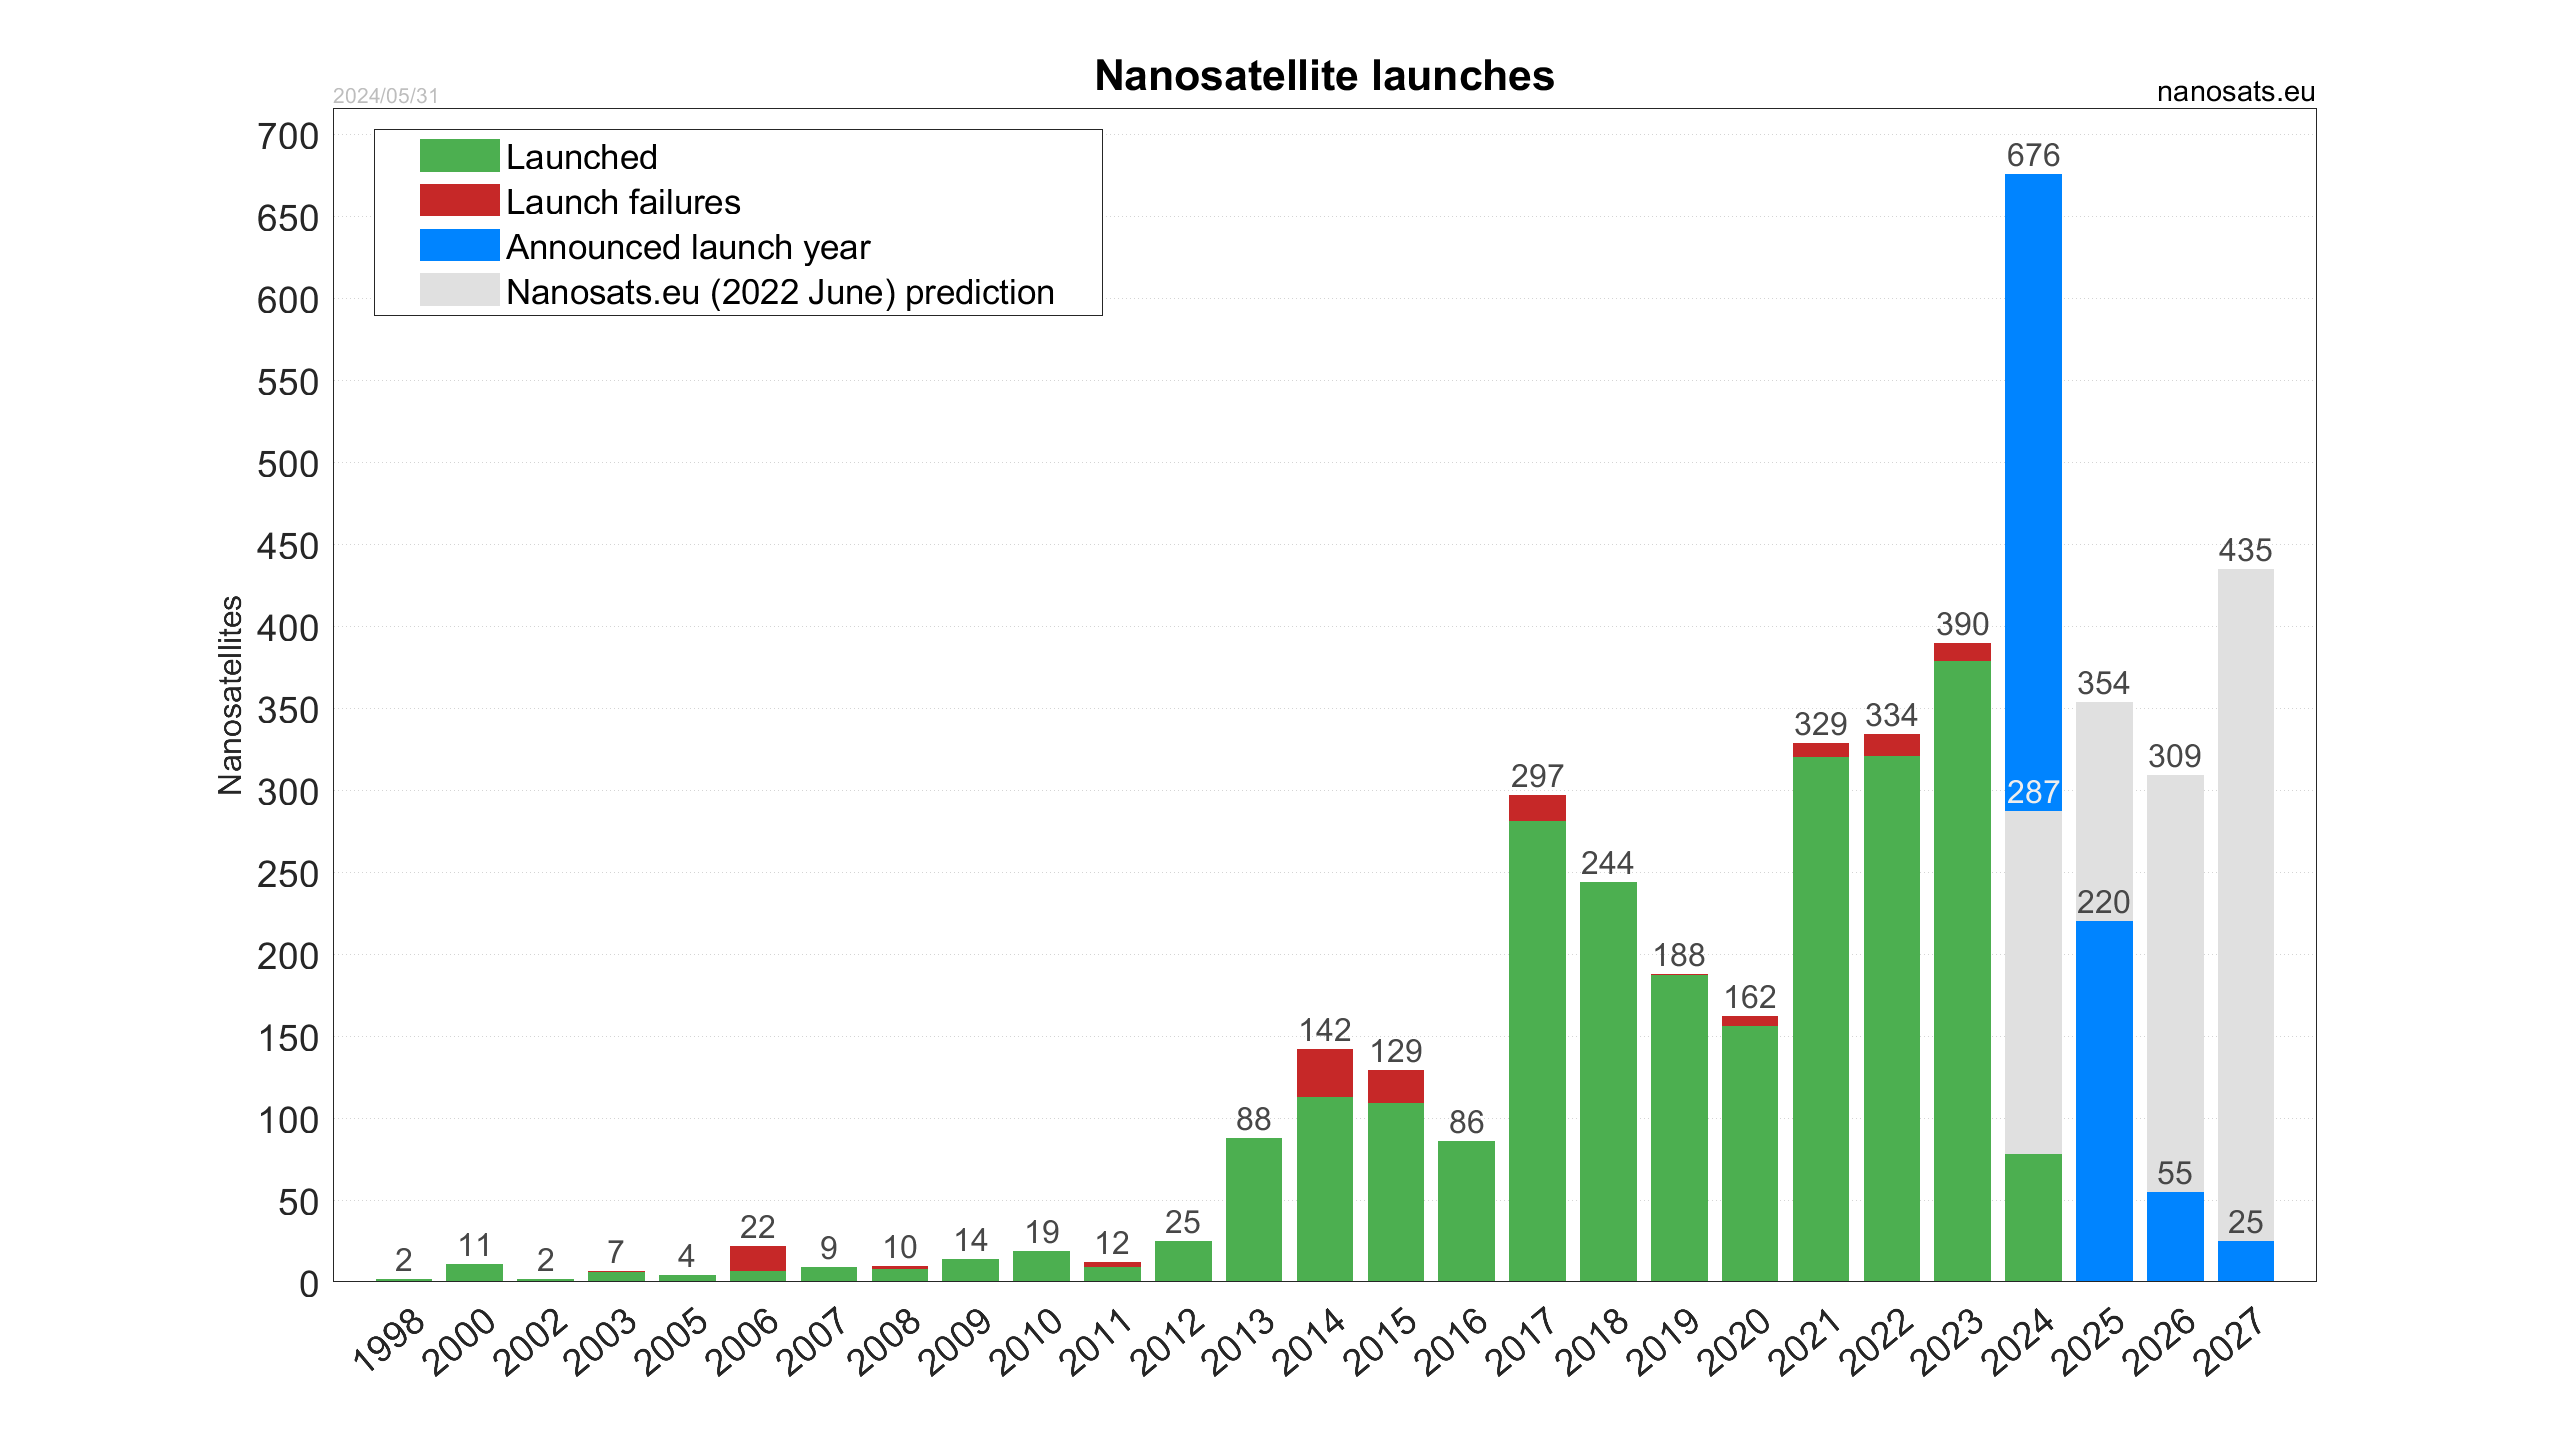
\includegraphics[width=1\textwidth]{Nanosats_years_2024-05-31_large.png}
	\caption{Cantidad de nanosatélites lanzados a través de los años \cite{ref1}.}.
	\label{fig:nanosats}
\end{figure}

Dentro de estos nanosatélites, una aplicación con gran porcentaje de ocurrencia en el ámbito comercial está enfocado en la observación terrestre mediante la utilización de cargas útiles ópticas \cite{ref3}. Esta aplicación consiste en la captura de imágenes de la superficie terrestre utilizando sensores que detectan distintas partes del espectro electromagnético. Estos sensores ópticos funcionan al detectar la luz reflejada (generalmente luz infrarroja cercano o visible) en la superficie de la Tierra \cite{ref4}.

Para llevar a cabo este tipo de misión, se requiere de una capacidad de apuntamiento con el fin de cumplir el objetivo de capturar imágenes con la calidad y resolución requeridas. El concepto de apuntamiento se define como la capacidad del satélite para ajustar su actitud, logrando un cambio de orientación hacia un objetivo deseado \cite{ref5}. 

Para determinar y/o caracterizar la capacidad de apuntamiento, es necesario medir y evaluar su desempeño a través de los Measures of Performance (MoP) relevantes para las misiones de observación terrestre. En estudios anteriores \cite{ref5, ref6, ref7, ref8} , se proporciona una definición cualitativa de los siguientes MoP de apuntamiento, los cuales están condicionados por la calidad del hardware y software (algoritmos de estimación y/o determinación de actitud) correspondientes al subsistema de determinación y control de actitud (ADCS):

\begin{itemize}
	\item Exactitud de apuntamiento \cite{ref5,ref7}: Definido como el error absoluto entre la orientación requerida.
	\item Drift \cite{ref5}: Se refiere a cuánto puede desviarse un vehículo con el tiempo. Este parámetro es crucial cuando se necesita mantener una dirección específica y se deben hacer correcciones solo ocasionalmente para evitar que el vehículo se desvíe significativamente de su curso deseado. Representado mediante ángulos por hora [°/hr].
	\item Jitter \cite{ref9,ref10}: Se representa como las vibraciones mecánicas de alta frecuencia que provocan una visualización difuminada en la cámara y se cuantifica como la densidad espectro potencia del filtro pasa alto de la respuesta a la estabilización del satélite.
	\item Agilidad \cite{ref11}: Se describe como el tiempo de asentamiento con el cual se estabiliza el CubeSat a la orientación deseada, representada en segundos. Generalmente mediante una banda de asentamiento del 5\%.
\end{itemize}

En conjunto con los parámetros de apuntamiento, es crucial considerar los System Engineering (SE) envelopes específicos para el tipo de misión y satélite en uso. Estos SE envelopes son restricciones técnicas y operativas que deben ser consideradas durante las fases de diseño, desarrollo y operación del CubeSat. Los parámetros clave de estos envelopes incluyen la potencia eléctrica, la masa, el tamaño/volumen y el costo.

Los SE envelopes se definen principalmente en función de la carga útil, que es el punto de partida para el diseño y desarrollo de los demás subsistemas del satélite, especialmente el Attitude Determination and Control System (ADCS), que es fundamental para el apuntamiento del satélite \cite{ref8}.

Dado que los CubeSats tienen restricciones de masa y volumen (de acuerdo con el estándar de unidades), y se busca minimizar costos al limitar el costo de componentes y reducir la superficie de paneles solares (y por ende la potencia y energía disponible), es necesario establecer requerimientos específicos para los SE envelopes del satélite y los parámetros de apuntamiento. Esto se debe hacer de acuerdo con la complejidad de la misión de observación terrestre, para encontrar un equilibrio óptimo entre estos aspectos y satisfacer las necesidades de la misión.

Por lo tanto, es esencial definir claramente los aspectos de la misión, tales como la dinámica orbital (incluyendo los parámetros orbitales y las perturbaciones en órbita baja (LEO)) y la geometría del satélite, así como las limitaciones y capacidades del ADCS. Esto permitirá conocer el costo asociado a la misión y su desempeño en términos de apuntamiento. La Figura~\ref{fig:bloques01} presenta un diagrama que ilustra esta interacción, mostrando una visualización gráfica de los parámetros de costo y rendimiento.

\begin{figure}[h]
	\centering    
	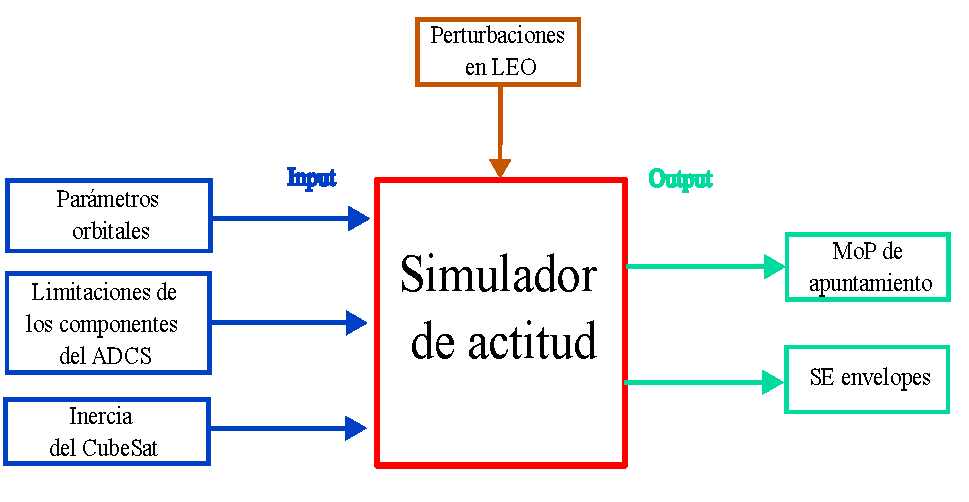
\includegraphics[width=0.9\textwidth]{diagrama memoria1234.pdf}
	\caption{Representación gráfica de la relación entre aspectos de la misión respecto a costo y rendimiento (Elaboración propia).}
	\label{fig:bloques01}
\end{figure}

Existen estudios que simulan diversos aspectos del Attitude Determination and Control System (ADCS), incluyendo los componentes físicos \cite{ref12}, algoritmos de determinación de actitud \cite{ref13} y controladores \cite{ref14}. En estos trabajos, se analizan y comparan los diferentes elementos del ADCS para identificar cuáles ofrecen mejores rendimientos, con un enfoque particular en el budget de potencia, que es uno de los factores más relevantes. Además, también se han realizado estudios en los que se simula el ADCS completo de un CubeSat, especificando tanto su diseño como los resultados de su rendimiento \cite{ref15,ref16,ref17}.

Por otro lado, en \cite{ref18} y \cite{ref19} se presentan herramientas y simuladores capaces de implementar la dinámica orbital y de actitud, proporcionando una interfaz gráfica que visualiza los movimientos traslacionales y rotacionales, así como los modelos de perturbación correspondientes. Estas herramientas permiten cuantificar algunos de los Measures of Performance (MoP) de apuntamiento y evaluar los costos en función de los SE envelopes. La herramienta mencionada en \cite{ref18}, llamada Spacecraft Control Toolbox, está dividida en tres secciones según los requerimientos de las misiones. Tiene la capacidad de generar resultados relacionados con la dinámica rotacional del satélite, incluye una interfaz gráfica y, en su versión económica, estima el consumo de energía. En sus versiones académicas o profesionales, permite además recuperar errores de apuntamiento y modelar sensores y actuadores.

Además, en \cite{ref19} se presentan herramientas y plantillas disponibles en el Aerospace Blockset de MATLAB, que permiten modelar un CubeSat siguiendo especificaciones del satélite y de la órbita, y realizar simulaciones utilizando la herramienta Simulink Animation 3D para visualizar los resultados.

También existen herramientas como Valispace, cuyo propósito es principalmente el análisis de budgets de ingeniería. Un ejemplo común de su uso se describe en \cite{ref20}. Este tipo de software ofrece una visión integral del análisis de satélites, abarcando costos temporales, monetarios y de potencia, al utilizar funciones que integran los requisitos de los subsistemas involucrados.

Finalmente, existe un entorno de simulacion gratuito de la universidad de Colorado para sistemas de naves espaciales. Esta es una herramienta muy utilizada en la investigación académica y en proyectos relacionados con la simulación de dinámicas y control de vehículos espaciales de alta dificultad de uso, al combinar distintos topicos y lenguajes de programación en su arquitectura \cite{ref36}.
%falta mencionar el software de Elias (gratuito pero dificil de utilizar para el usuario)

Teniendo esto en cuenta, el simulador propuesto se perfila como una herramienta valiosa para el análisis del ADCS de un CubeSat. Al proporcionar la información adecuada del satélite,su órbita y el análisis especifico requerido, el simulador permitirá obtener tanto el rendimiento como el costo asociado al apuntamiento. Además, contribuirá al desarrollo tecnológico de CubeSats de manera simple y eficiente, utilizando componentes basados en CubeSats comerciales en la actualidad, todo dentro de un entorno de programación de libre acceso como Python. Asimismo, el simulador será capaz de ofrecer las características del ADCS necesarias para alcanzar un rendimiento o costo específico, según los parámetros definidos por el usuario. Un resumen de lo que se busca una vez implementado la suite de simulacion de la Figura~\ref{fig:bloques01}, se representa en la Figura~\ref{fig:bloques02}.

\begin{figure}[h]
	\centering    
	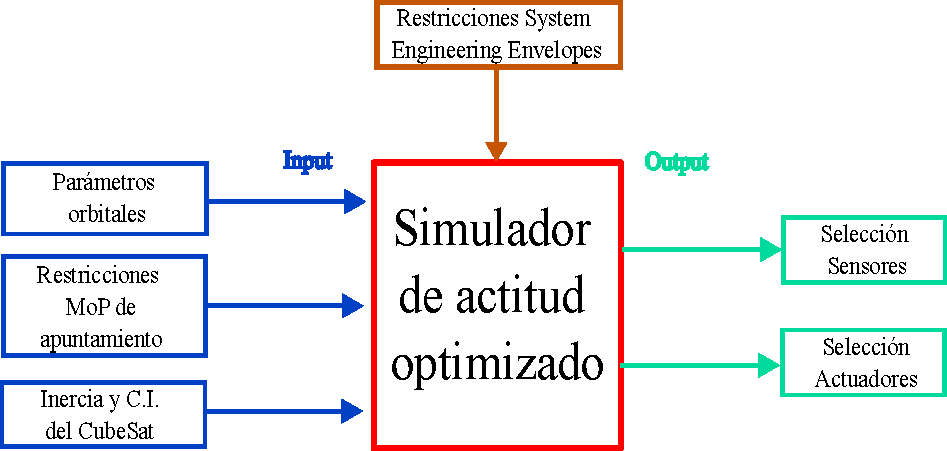
\includegraphics[width=0.9\textwidth]{bloque02.pdf}
	\caption{Solución propuesta para la suite de simulación optimizada (Elaboración propia).}
	\label{fig:bloques02}
\end{figure}

\subsection{Hipótesis}
Se postula que el diseño e implementación de una suite de simulación que modele el ambiente espacial y el ADCS, en conjunto con un algoritmo capaz de optimizar los parámetros de rendimiento y los SE envelopes, mejorará la eficacia operativa de las misiones CubeSat al seleccionar el subconjunto óptimo de componentes físicos necesarios.

\subsection{Objetivos}
\textit{\underline{Objetivo General:}} Diseñar e implementar una suite de simulación que modele el ambiente espacial y el ADCS de un CubeSat comercial de observación terrestre en órbitas bajas, capaz de optimizar los MoP de apuntamiento en función de los SE envelopes de los componentes físicos.

\textit{\underline{Objetivos Especificos:}}

\begin{itemize}
	\item OE1: Desarrollar un marco teórico robusto sobre el modelamiento del ambiente espacial y del ADCS de un CubeSat, enfocado en aplicaciones de observación terrestre, basadas en referencias publicadas después del año 2010.
	\item OE2: Desarrollar un modelo de ambiente espacial que permita calcular los vectores de posición y velocidad del CubeSat, junto con un modelo de actitud que incluya al menos dos sensores y dos actuadores del ADCS.
	\item OE3:Implementar un algoritmo de estimación para el modelo dinámico del CubeSat con un margen de error inferior al 5\%.
	\item OE4: Diseñar al menos un  controlador que permita control de actitud en función de los actuadores implementados en la suite de simulación.
	\item OE5: Seleccionar e implementar un algoritmo de optimización no lineal capaz de optimizar los MoP de apuntamiento en función de los SE envelopes en la suite de simulación.
	\item OE6: Verificación cuantitativa de la suite de optimización utilizando datos empíricos del SUCHAI-3 en base a los MoP de apuntamiento obtenidos y los SE envelopes de sus componentes físicos actuales
\end{itemize}




\subsection{Metodología}

OE1: Desarrollar el marco teórico relacionado con el ADCS y el ambiente espacial en el simulador mediante la revisión de trabajos previos. Se recopilará información de artículos y estudios sobre la determinación y control de actitud en CubeSats, junto con el estado del arte y las especificaciones técnicas de componentes disponibles en sitios web de fabricantes, para verificar la correcta implementación de los modelos y su similitud con estudios anteriores.

OE2: Implementar el propagador SGP4 para calcular los vectores de posición y velocidad del CubeSat, teniendo en cuenta las perturbaciones orbitales en órbitas bajas. En cuanto a los modelos dinámicos de actitud, se simularán las fuerzas magnéticas y el vector solar para representar el comportamiento de sensores como el magnetómetro y el sensor solar. Los actuadores considerados en los modelos serán el magnetorquer y la rueda de reacción en los ejes del CubeSat.

OE3: Estimar los cuaterniones y las velocidades angulares del CubeSat utilizando un filtro de Kalman extendido. Este filtro será aplicado al modelo dinámico lineal discreto, integrando el magnetorquer y las ruedas de reacción. Se emplearán las mediciones simuladas de los sensores para validar las estimaciones y se evaluará la precisión de las mismas mediante el cálculo del error cuadrático medio (MSE).

OE4: Diseñar un controlador PD o LQR dentro de la suite de simulación. Una vez implementados ambos controladores, se seleccionará el de mejor rendimiento en función de los MoP de apuntamiento bajo las mismas condiciones de simulación.

OE5: Realizar una revisión de optimizadores no lineales convexos disponibles en Python, con el objetivo de encontrar una solución óptima que maximice el rendimiento y minimice el costo en función de las entradas y requisitos del usuario. Se evaluarán herramientas como scipy.optimize, pyomo y cvxpy para determinar el optimizador más adecuado.

OE6: Verificar la suite de simulación utilizando datos empíricos del SUCHAI-3. Se compararán los resultados de la simulación con los parámetros reales de rendimiento de los componentes físicos y se evaluará la proximidad de los resultados obtenidos por la suite de optimización con los datos reales, determinando el conjunto óptimo de sensores y actuadores.
                                                                     \subsection{Carta Gantt}                                                                                                                                                                                                               
El proyecto sigue una estructura definida contenida en la carta Gantt mostrada en el Anexo A.

\section{Marco Teórico}

\subsection{Sistemas de referencia}

Para describir la dinámica orbital, de actitud y el diseño del ADCS, es necesario la definición de los marcos de referencia a utilizar. Su selección obedece a criterios descritos a continuación.

\begin{itemize}
	\item \textbf{Sistema de referencia body o del cuerpo \cite{ref21}}: La dinámica relativa de actitud se describe con respecto al marco de referencia del cuerpo en el CubeSat, desde la cual se realizan las mediciones, debido a que los sensores de actitud están fijados a su cuerpo. Para los marcos de referencia del cuerpo, el eje z apunta en la dirección del momento de inercia más alto, y los ejes x e y son paralelos a los vectores de área de las caras de la nave espacial, apuntando todos en las direcciones principales del satélite, como se observa gráficamente en la Figura~\ref{fig:body}.
	
	\begin{figure}[h]
		\centering    
		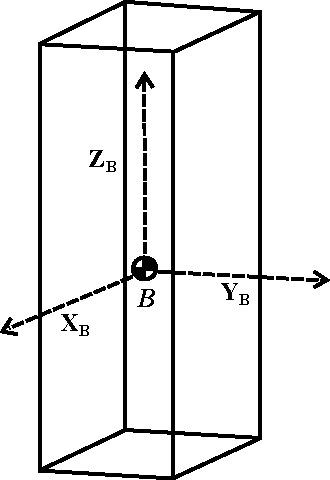
\includegraphics[width=0.28\textwidth]{body.pdf}
		\caption{Marco de referencia del cuerpo (Elaboración propia).}
		\label{fig:body}
	\end{figure}
	
	\item \textbf{Sistema de referencia inercial \cite{ref21,ref22}}: El Sistema de referencia inercial utilizado es el Earth Centered Inertial (ECI) debido a la necesidad de obtener vectores respecto a un marco de referencia no rotativo (asumiendo problema de dos cuerpos entre la Tierra y el satélite). El eje X apunta en la dirección del equinoccio de primavera. El plano XY es el plano ecuatorial de la Tierra, y el eje Z coincide con el eje de rotación de la Tierra y apunta hacia el norte. Este sistema de referencia se puede apreciar en la Figura~\ref{fig:ECI}.
	
	\begin{figure}[H]
		\centering    
		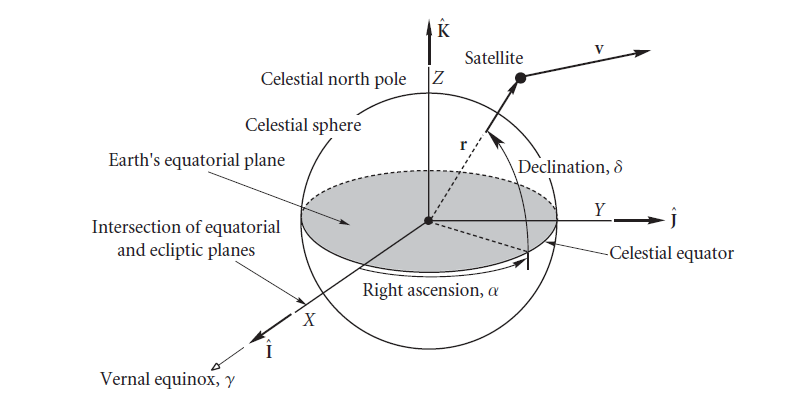
\includegraphics[width=0.8\textwidth]{ECI.png}
		\caption{Marco de referencia inercial ECI \cite{ref22}.}
		\label{fig:ECI}
	\end{figure}
	
	\item \textbf{Sistema de referencia LVLH o Roll-Pitch-Yaw  \cite{ref23}}: Se define un sistema coordenado que mantiene su orientación relativa a la Tierra a medida que la nave espacial se mueve en su órbita. Estas coordenadas son conocidas como roll, pitch y yaw (RPY), \textit{Local Vertical Local Horizontal} (LVLH) u orbital como también será llamada en este trabajo y se ilustra en la Figura~\ref{fig:RPY}. En este sistema, el eje yaw se dirige hacia el nadir (es decir, hacia el centro de la Tierra), el eje pitch se dirige hacia la normal negativa de la órbita, y el eje roll es perpendicular a los otros dos, tal y como se muestra en la Ecuación~\ref{eq:RPY}. Se utilizará este Sistema de referencia para notar la posición ideal de la carga útil.
	 \begin{equation}
		\hat{R} = \hat{P} \times \hat{Y}
		\label{eq:RPY}
	\end{equation} 


	\begin{figure}[H]
		\centering    
		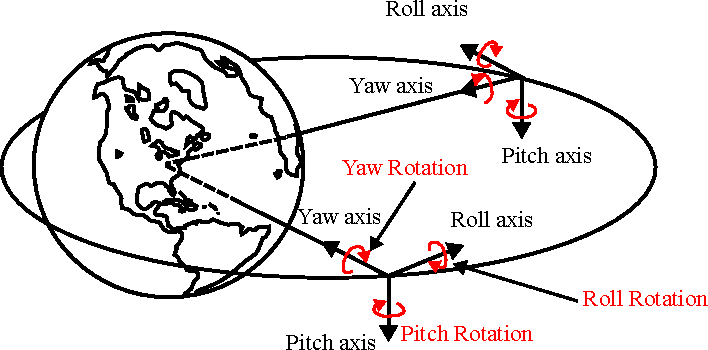
\includegraphics[width=0.6\textwidth]{RPY.pdf}
		\caption{Marco de referencia inercial RPY \cite{ref23}.}
		\label{fig:RPY}
	\end{figure}	
	
\end{itemize}


\subsection{Dinámica orbital}

Para el modelamiento de la suite de simulación se debe conocer el significado de los parámetros orbitales que se entregara como entrada, así como las ecuaciones que gobiernan el movimiento del satélite a través de la Tierra y las perturbaciones presentes a baja altura.

\subsubsection{Parámetros orbitales}

Si la masa de un satélite se considera insignificante en comparación con la masa de la Tierra, y bajo el supuesto de que la Tierra es esféricamente simétrica, la aceleración \( \ddot{\mathbf{r}} \) de un satélite está dado por la ley de gravedad de Newton descrita a continuación:

\begin{equation}
	\ddot{\mathbf{r}} = -\frac{GM_E}{r^3} \mathbf{r}
	\label{eq:Newton}
\end{equation}

Donde $\mathbf{r}$ es el vector posición entre el satélite y la Tierra y $GM_E$ es conocida como la constante de gravitacional de la Tierra y está dada por:

\begin{equation}
	\mu = {GM_E} = 398600,4418  [\frac{{km}^3}{{s}^2}]
	\label{eq:cteGrav}
\end{equation}

Al resolver la Ecuación~\ref{eq:Newton}, se obtiene la posición y la velocidad del del satélite respecto a la Tierra en cualquier instante de tiempo dependiendo del sistema de referencia a utilizar. Si bien se tiene una cuantificación del posicionamiento y el movimiento del satélite, generalmente se utiliza otra caracterización para definir la órbita, utilizando los elementos keplerianos, los cuales se presentan en la Figura~\ref{fig:kepler}.

\begin{figure}[H]
	\centering    
	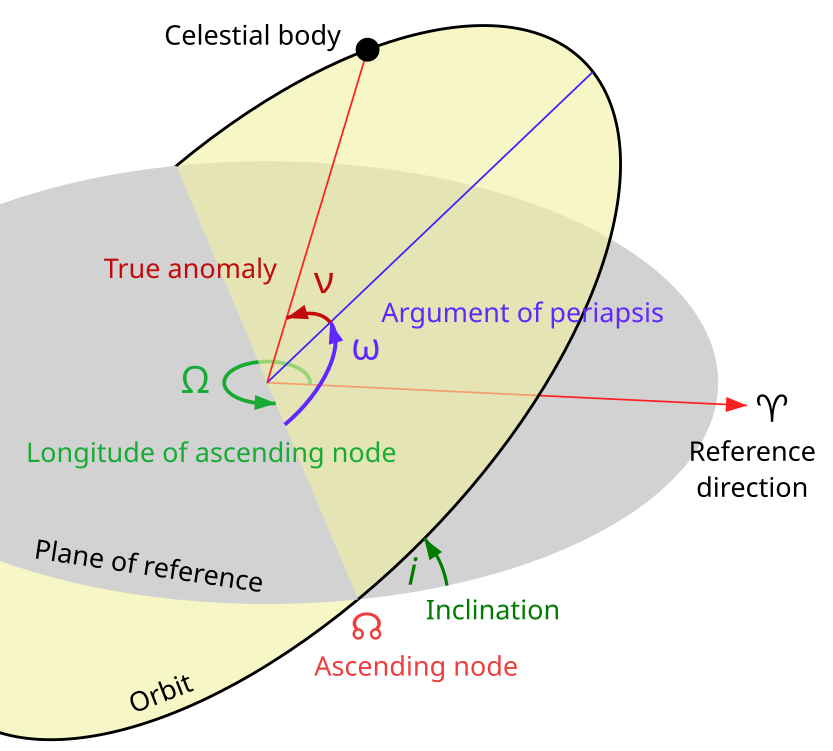
\includegraphics[width=0.45\textwidth]{keplerianos.png}
	\caption{Elementos keplerianos \cite{ref24}.}
	\label{fig:kepler}
\end{figure}

Dichos elementos se definen brevemente a continuación, los que se pueden determinar desde la posición y la velocidad del satélite respecto a la Tierra mediante relaciones matemáticas obtenidas en \cite{ref22}.


\begin{itemize}
	\item \textbf{Excentricidad (e)}: Describe el alargamiento de la órbita. Si presenta valores entre 0 y 1 tendrá forma de elipse. Si es igual a 0 representa una órbita circular, mientras que si es igual a 1 tiene forma de parábola. Para casos mayores a 1 se presentan orbitas de trayectoria hiperbólica.
	
	\item \textbf{Semieje mayor (a)}: Es la distancia entre el periapsis (distancia más cercana entre el satélite y la Tierra) y el apoapsis (distancia más lejana entre el satélite y la Tierra) dividido por 2. Representa el radio para orbitas circulares.
	
	\item \textbf{Inclinación (i)}: Inclinación vertical de la elipse con respecto al plano de referencia (plano ecuatorial).
	
	\item \textbf{Right Ascension of the Ascending Node (RAAN $\Omega$)}: Inclinación vertical de la elipse con respecto al plano de referencia (plano ecuatorial).	
	
	\item \textbf{Argumento del periapsis ($\omega$)}: Se define la orientación de la elipse en el plano orbital, como un ángulo medido desde el nodo ascendente a la periapsis.
	
	\item \textbf{Anomalía verdadera  ($\nu$)}: Define la posición del cuerpo orbitante a lo largo de la elipse en un tiempo específico.
\end{itemize}

\subsubsection{Perturbaciones presentes en LEO}

Existen perturbaciones en el espacio que afectan a los satélites en órbita, de las cuales algunas tienen más relevancia a bajas altura respecto de la Tierra. Estas se muestran a continuación:

\textbf{Gravedad no esférica \cite{ref25}}: La Tierra no es una esfera perfecta y la masa se distribuye de manera no uniforme. A diferencia de las simplificaciones que se aplican a menudo en órbitas altas, donde la influencia de la Tierra se aproxima a una esfera, en LEO la distribución irregular de la masa terrestre y las variaciones en la altitud pueden generar perturbaciones significativas en las trayectorias de los satélites. Por lo tanto, como la fuerza de gravedad depende directamente de la masa, el campo gravitatorio reflejará esta falta de uniformidad.

Para lograr modelar la gravedad no esférica se utiliza una expansión armónica esférica, con modelos como el geopotencial que descompone el campo gravitatorio terrestre en una serie de términos, cada uno correspondiente a una armonía esférica y su respectiva magnitud. Dentro de los coeficientes utilizados dentro del modelo recién mencionado están los “J”, siendo el J2 el principal para modelar el achatamiento de la Tierra. Otros J como el J3, J4, etc., modelan a mayor detalle la distribución másica de la Tierra.

\textbf{Efectos atmosféricos \cite{ref26}}: Los efectos del arrastre y el oxígeno atómico (O) tienen implicancias para los satélites de baja altura (menor a 600 km). El arrastre se define como una fuerza resistiva que actúa sobre un objeto en movimiento a través de un fluido y tiende a disminuir su velocidad, cuyas implicancias son que acorta la vida útil del satélite. El arrastre depende de la densidad, la velocidad y también variará según cómo cambie la atmósfera (se expanda o se contraiga) debido a la variación en la actividad sola. 

Por otro lado, debido a que en la atmosfera superior existe una mayor radiación, esto hace que se disocien los átomos de $O_{2}$ a O, los cuales son muy reactivos y potencialmente dañinos, degradando las superficies del CubeSat e interfiriendo con los sensores para la determinación de actitud.

\subsection{Cinemática y dinámica de actitud}

Para la cinemática y dinámica de actitud, el satélite ya no se asume como una partícula perturbada (como en el caso de la dinámica orbital), sino como un cuerpo rígido con masa. Con esto aparecen conceptos que serán definidos en esta sección.

\subsubsection{Actitud de un satélite y sus representaciones}

La actitud de un satélite se refiere a la orientación o posición que mantiene en el espacio mientras órbita alrededor de la Tierra u otro cuerpo celeste. Para describir esta actitud, se utilizan diversas representaciones matemáticas que permiten definir de manera precisa su orientación en el marco de referencia del cuerpo respecto al inercial, las cuales se presentan a continuación \cite{ref23}:


\begin{itemize}
	\item \textbf{Direction Cosine Matrix (DCM)}: Esta parametrización utiliza una matriz 3x3 para representar la orientación del satélite en relación con un sistema de referencia fijo. La matriz contiene nueve elementos que son los cosenos directores de los ejes del satélite en relación con los ejes de referencia. Es una representación matemáticamente precisa pero no es tan intuitiva como otras. Dicha representación se visualiza en la Figura~\ref{fig:DCM}.
	
	\begin{figure}[H]
		\centering    
		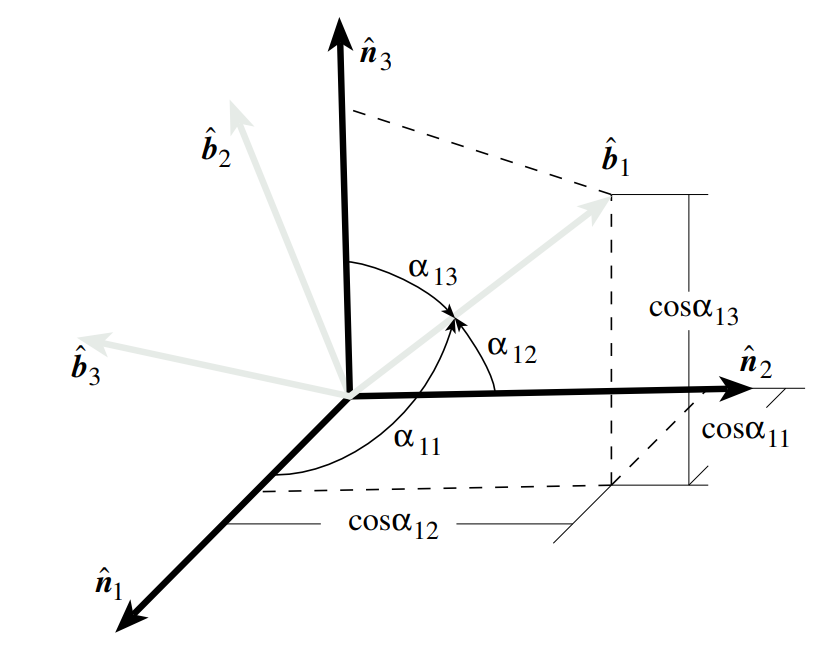
\includegraphics[width=0.45\textwidth]{DCM.png}
		\caption{Representación gráfica de la primera fila de la matriz de cosenos directores \cite{ref27}.}
		\label{fig:DCM}
	\end{figure}
	
	\item \textbf{Euler axis/angle}: En esta parametrización, se utiliza un vector tridimensional (el eje de Euler) junto con un ángulo para describir la orientación. El vector de Euler define el eje de rotación, mientras que el ángulo especifica la magnitud de la rotación alrededor de ese eje, como se muestra en la Figura~\ref{fig:axis_angle}. Es útil para representar giros simples y es intuitiva. 
	
	\begin{figure}[H]
		\centering    
		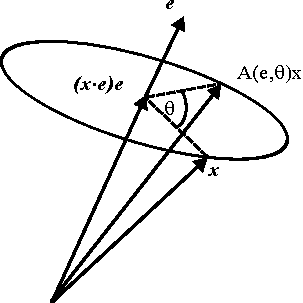
\includegraphics[width=0.3\textwidth]{axis_angle.pdf}
		\caption{Representación de un cambio de orientación en Euler axis/angle de x \cite{ref25}.}
		\label{fig:axis_angle}
	\end{figure}	
	
	\item \textbf{Euler angles}: Esta parametrización describe la orientación mediante tres ángulos, generalmente llamados phi ($\phi$), theta ($\theta$) y psi ($\psi$), que representan las rotaciones en torno a los ejes específicos (por ejemplo, X, Y y Z). Se presenta en la Figura~\ref{fig:euler_angles} las rotaciones realizadas por esta parametrización. 
	
	\begin{figure}[H]
		\centering    
		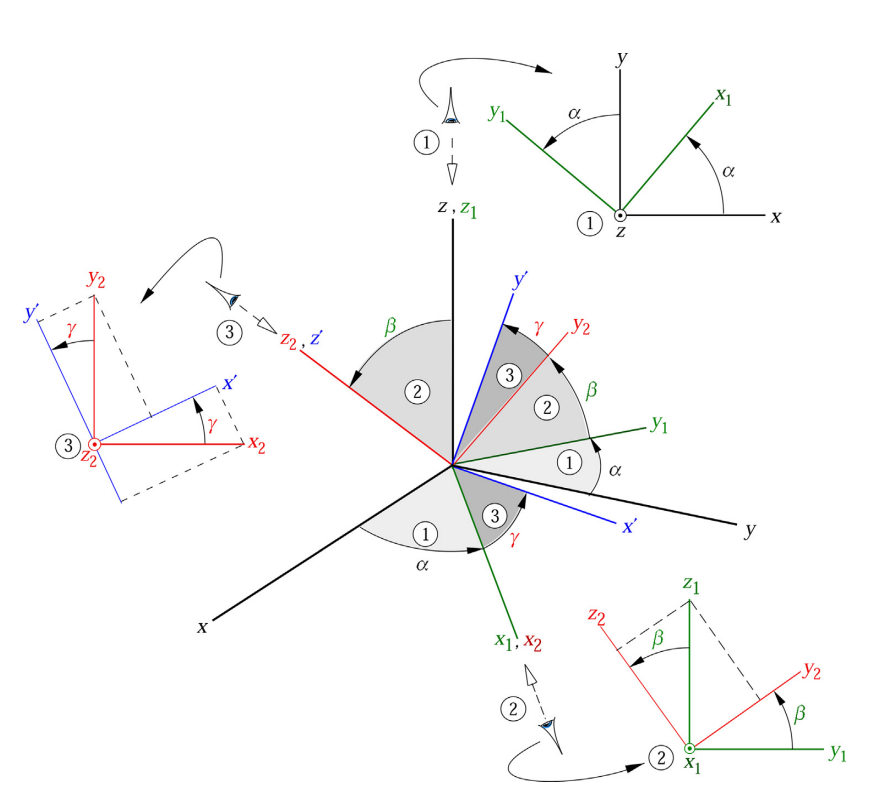
\includegraphics[width=0.6\textwidth]{euler_angles.png}
		\caption{Secuencia clásica de Euler de tres rotaciones que transforman xyz en x’y’z’ \cite{ref22}.}
		\label{fig:euler_angles}
	\end{figure}
	
	\item \textbf{Cuaternión}: Esta parametrización utiliza cuatro parámetros para representar la orientación, siendo tres de estas vectoriales y una escalar. Se discutirá más a fondo en la siguiente sección. 			
\end{itemize}

\subsubsection{Cuaterniones y cinemática de cuaterniones}

En este trabajo, la parametrización seleccionada para la descripción de la actitud es el cuaternión. Los cuaterniones tienen múltiples ventajas en comparación con otras parametrizaciones de actitud. Por ejemplo, en la parametrización de ángulos de Euler, la propagación de la actitud no es suave. Sin embargo, esta suavidad es fundamental para el correcto funcionamiento de métodos de estimación como el Filtro de Kalman \cite{ref23}.

Por otro lado, la desventaja de la parametrización de la matriz de cosenos directores es que conduce a una descripción de la actitud utilizando nueve elementos no independientes, y cumple con seis restricciones impuestas por la ortogonalidad de la matriz de actitud que son redundantes.
La cantidad mínima de elementos que se pueden utilizar para describir la actitud sin singularidades son cuatro. A partir del hecho de que cualquier rotación puede describirse utilizando un solo eje de rotación y un ángulo que describe la rotación alrededor de este eje, el cuaternión se define mediante 4 elementos, con una parte vectorial y una parte escalar como se muestra a continuación \cite{ref22}:

\begin{equation}
	\hat{q} = \begin{bmatrix}
		q_0 \\
		q_1 \\
		q_2 \\
		q_3
	\end{bmatrix}
	= \begin{bmatrix}
		\mathbf{q} \\
		q_3
	\end{bmatrix}
	= \begin{bmatrix}
		\sin\left(\frac{\theta}{2}\right) \hat{u} \\
		\cos\left(\frac{\theta}{2}\right)
	\end{bmatrix}
	\label{eq:cin_quat}
\end{equation}

La expresión \( \mathbf{q} \) es la parte vectorial \( \mathbf{q} = q_0 \hat{i} + q_1 \hat{j} + q_2 \hat{k} \), y \( q_3 \) es la parte escalar. La representación mostrada corresponde a un cuaternión pasivo, el cual se utiliza para rotar el sistema de coordenadas en sí (sin rotar el vector). Si se desea rotar el vector sin rotar el sistema de coordenadas, se utiliza un cuaternión activo, y se obtiene cambiando la componente escalar al inicio, tal y como se muestra en la siguiente expresión:

\[
\hat{q} = \begin{bmatrix}
	q_3 \\
	q_0 \\
	q_1 \\
	q_2
\end{bmatrix}
= \begin{bmatrix}
	q_3 \\
	\mathbf{q}
\end{bmatrix}
\]

Sabiendo esto, se puede definir la cinemática de la actitud del satélite utilizando cuaterniones mediante la Ecuación ~\ref{eq:cin_omega}, sabiendo que \( \omega_0 \), \( \omega_1 \) y \( \omega_2 \) son las velocidades angulares en el marco de referencia cuerpo del satélite:

\begin{equation}
	\frac{d\hat{q}}{dt} = \frac{1}{2}
	\begin{bmatrix}
		0 & -\omega_2 & \omega_1 & -\omega_0 \\
		\omega_2 & 0 & -\omega_0 & -\omega_1 \\
		-\omega_1 & \omega_0 & 0 & -\omega_2 \\
		\omega_0 & \omega_1 & \omega_2 & 0
	\end{bmatrix}
	\hat{q}
	\label{eq:cin_omega}
\end{equation}

Además, se tiene la multiplicación de cuaterniones, la cual será útil para representar las rotaciones entre los sistemas de referencia y aproximaciones discretas que utilizan esta operación, la cual se representa en la Ecuación~\ref{eq:quat_mult}:

\begin{equation}
	\hat{q} \cdot \hat{r} =
	\begin{bmatrix}
		q_3 r_0 + q_0 r_3 + q_1 r_2 - q_2 r_1 \\
		q_3 r_1 + q_1 r_3 + q_2 r_0 - q_0 r_2 \\
		q_3 r_2 + q_2 r_3 + q_0 r_1 - q_1 r_0 \\
		q_3 r_3 - q_0 r_0 - q_1 r_1 - q_2 r_2
	\end{bmatrix}
	\label{eq:quat_mult}
\end{equation}

Si bien esta parametrización no tiene una representación física obvia, se puede describir la rotación del satélite a través del tiempo mediante un integrador numérico, sabiendo la condición inicial tanto del cuaternión como de la velocidad angular.

\subsubsection{Dinámica de actitud}

La ecuación que describe la variación del vector momento angular a través del tiempo para un torque aplicado en un marco de referencia del cuerpo representa la dinámica de actitud y se muestra en la Ecuación~\ref{eq:vect_dot} \cite{ref22}:

\begin{equation}
	I \frac{d\boldsymbol{\omega}}{dt} = - \boldsymbol{\omega} \times I \boldsymbol{\omega} + \boldsymbol{\tau}
	\label{eq:vect_dot}
\end{equation}

Sabiendo que \( \boldsymbol{\omega} \) es el vector de velocidad angular instantánea en el cuerpo, \( I \) son los momentos principales de inercia y \( \boldsymbol{\tau} \) son los torques aplicados, esta ecuación se puede representar también según sus componentes en \( i \), \( j \) y \( k \):

\[
\dot{\omega}_0 = \frac{\omega_1 \omega_2 (I_y - I_z)}{I_x} + \frac{\tau_x}{I_x}
\]
\[
\dot{\omega}_1 = \frac{\omega_0 \omega_2 (I_x - I_z)}{I_y} + \frac{\tau_y}{I_y}
\]
\[
\dot{\omega}_2 = \frac{\omega_0 \omega_1 (I_x - I_y)}{I_z} + \frac{\tau_z}{I_z}
\]

Los torques externos son los provocados por los actuadores y por perturbaciones externas en orbitas de baja altura. Las ultimas mencionadas generalmente se simplifican a relaciones para el peor de los casos analizados. Estas perturbaciones que afectan a la dinámica rotacional del satélite son cuatro y se discuten a fondo en el Anexo \ref{ap:Z2}.

\subsection{Subsistema de determinación y control de actitud}

El subsistema de determinación y control de actitud de un CubeSat es el responsable de determinar su orientación en el espacio y controlarla respecto a un objetivo durante un periodo específico. También se requiere para sobrevivir en el entorno espacial, controlando el satélite en orientaciones tales que se genere energía apuntando las celdas fotovoltaicas hacia el sol.

El proceso para poder describir el movimiento del satélite se describe en tres pasos o procesos los cuales son llamados Guidance, Navigation and Control (GNC). Cada uno se describe según los componentes del ADCS, como se muestra a continuación \cite{ref28}:

\begin{itemize}
	\item Navigation: Es el primer paso por seguir, y determina la actitud del satélite y la tasa de rotación mediante los sensores tanto inerciales como de medición externa. Responde a la pregunta: ¿Dónde está el satélite?
	\item Guidance: Al determinar la actitud con los sensores, se utilizan algoritmos de determinación de actitud para estimar la orientación tanto inicial como a través del tiempo, para posteriormente utilizar algoritmos de determinación de actitud para estimar la orientación del satélite. Responde a la pregunta: ¿Hacia dónde quiere ir el satélite?
	\item Control: Ya conocido hacia donde quiere ir el satélite, se genera el cambio de actitud mediante la implementación de torques utilizando controladores en conjunto con actuadores. Responde a la pregunta: ¿Cómo dirijo el satélite hacia allá?
\end{itemize}

\subsubsection{Navigation (Sensores)}

Para la determinación de actitud se utilizan componentes físicos llamados sensores, los cuales miden su orientación en base a la inercia del satélite como también observando las estrellas circundantes/cuerpos celestes o midiendo fuerzas representativas de una posición en particular\cite{ref6}. Los sensores comúnmente utilizados en CubeSat se presentan en la Tabla~\ref{tab:sensores}, en conjunto con su descripción.


\begin{table}[h!]
	\centering
	\caption{Sensores utilizados en CubeSat \cite{ref6}.}
	\begin{tabular}{|l|p{10cm}|}
		\hline
		\textbf{Sensores} & \textbf{Descripción} \\ \hline
		Giroscopios & Los giroscopios miden la tasa de cambio de la orientación angular respecto al marco inercial del satélite [°/s]. Los giroscopios proporcionan información sobre los movimientos de rotación en los tres ejes (roll, pitch y yaw). \\ \hline
		Sensores de sol & Los sensores solares se utilizan para estimar la dirección del Sol en el marco de referencia del cuerpo del satélite. \\ \hline
		Magnetómetros & Los magnetómetros determinan el campo magnético de la Tierra, midiendo su dirección y su fuerza en [nT]. \\ \hline
		GPS & Mediante el receptor GPS se obtiene la posición tridimensional (latitud, longitud y altitud) con alta precisión. Esto permite al CubeSat conocer su ubicación en la órbita terrestre. \\ \hline
		Star Tracker & Un Star Tracker o contador de estrellas es un sistema de sensores cuya función principal es determinar con exactitud la actitud del CubeSat utilizando las estrellas circundantes como referencia. \\ \hline
	\end{tabular}
	\label{tab:sensores}
\end{table}

\subsubsection{Guidance (Algoritmos)}

En esta sección se proporciona una descripción de los diferentes métodos de determinación de actitud que se consideran para el simulador. En primera instancia, existen dos tipos principales de métodos de determinación de actitud. El primero de ellos es el método determinístico que utiliza la información de las lecturas de los sensores a lo largo de la misión y las comparan con modelos informáticos para calcular la actitud actual\cite{ref15}. Por otro lado, existen los estimadores recursivos que procesan las lecturas de sensores actuales y las compara con la última estimación de actitud para crear una nueva estimación.

\textbf{\underline{Enfoque determinista de la determinación de actitud}}

Para la determinación inicial de la actitud, se requiere un enfoque determinista. Existen varios algoritmos deterministas diferentes para la determinación de la actitud, describiendo algunos a continuación:

\textbf{TRIAD method}: La solución Tri-axial Attitude Determination (TRIAD) requiere dos conjuntos de vectores: un vector de observación de cada uno de los dos sensores ubicados en el satélite ($\mathbf{V_1}$ y $\mathbf{V_2}$), y un vector de referencia para cada observación en términos de su dirección de referencia inercial ($\mathbf{W_1}$ y $\mathbf{W_2}$). Con estos vectores se crean triadas de referencia ($\mathbf{M_{ref}}$) y de observación ($\mathbf{M_{obs}}$) descritas en la Tabla~\ref{tab:triad}.

\begin{table}[h!]
	\centering
	\caption{Descripción de las triadas de referencia y de observación.}
	\begin{tabular}{|c|p{10cm}|}
		\hline
		\textbf{Triada} & \textbf{Componentes de la triada} \\ \hline
		$\mathbf{M_{obs}} = \begin{bmatrix} \hat{r_1} & \hat{r_2} & \hat{r_3} \end{bmatrix}$ & $\hat{r_1} = \hat{V_1}; \, \hat{r_2} = \frac{\hat{V_1} \times \hat{V_2}}{|\hat{V_1} \times \hat{V_2}|}; \, \hat{r_3} = \hat{r_1} \times \hat{r_2}$ \\ \hline
		$\mathbf{M_{ref}} = \begin{bmatrix} \hat{s_1} & \hat{s_2} & \hat{s_3} \end{bmatrix}$ & $\hat{s_1} = \hat{W_1}; \, \hat{s_2} = \frac{\hat{W_1} \times \hat{W_2}}{|\hat{W_1} \times \hat{W_2}|}; \, \hat{s_3} = \hat{s_1} \times \hat{s_2}$ \\ \hline
	\end{tabular}
	\label{tab:triad}
\end{table}

Una vez que se calculan las tríadas de observación y referencia, se puede encontrar la solución TRIAD. Esta solución es la matriz de cosenos directores A que se define de la siguiente manera:

\[
A = M_{obs} (M_{ref})^T
\]

Esta matriz representa la rotación desde el marco de referencia del cuerpo del satélite al marco de referencia inercial fijo a la Tierra. Una vez que se conoce esta matriz, la actitud del satélite se puede expresar en términos del marco de referencia inercial fijo a la Tierra. Cuando se utiliza el método TRIAD, el sensor más exacto debe elegirse siempre como $V_1$ con su correspondiente vector de referencia $W_1$.

Por otro lado, existen algoritmos que ofrecen un mínimo error sin la necesidad de elegir el sensor más exacto como el $V_1$. Para ello, buscan resolver la ecuación de Wahba, la cual minimiza el error de determinación de actitud al asignarle pesos a los vectores de referencia y de observación. Estos métodos son el q-method y el QUEST \cite{ref15}, los cuales no se utilizarán durante este trabajo, ya que como se muestra en Vélez \cite{ref15}, el q-method presenta mayores errores en la determinación de actitud respecto a los otros algoritmos, mientras que QUEST en las mismas simulaciones tiene una calidad similar al TRIAD, con mayor costo computacional y una mayor dificultad de implementación.

\textbf{\underline{Enfoque recursivo de la estimación de actitud}}

Aunque se necesita un método determinista para la adquisición inicial de la actitud, un método recursivo a menudo es más eficiente para el mantenimiento del conocimiento de la actitud. A diferencia de los métodos deterministas, los métodos recursivos utilizan solo la lectura actual del sensor para calcular el error de actitud a partir de la estimación anterior. El método recursivo más común es un Filtro de Kalman.

Los Filtros de Kalman se utilizan para estimar los estados futuros de un sistema dinámico lineal afectado por ruido. El algoritmo consta de dos fases: la fase de predicción y la fase de actualización. Durante la fase de predicción, el filtro utiliza ecuaciones dinámicas del sistema preprogramadas para calcular la estimación a priori de la nueva actitud del satélite. Durante la fase de actualización, el filtro utiliza las lecturas actuales del sensor para determinar la estimación a posteriori de la actitud actual del satélite y calcular el error de estimación a partir de la predicción de la actitud.

Dado que el Filtro de Kalman tiene un proceso de dos pasos, utiliza un paso de tiempo discreto, k. La naturaleza discreta del Filtro de Kalman funciona bien para el CubeSat, ya que el paso de tiempo k puede configurarse fácilmente como el intervalo de tiempo entre las mediciones de los sensores. Sin embargo, el sistema dinámico del satélite al no ser lineal (dependiente del tiempo) se necesita utilizar el Filtro de Kalman Extendido (EKF). La naturaleza discreta del EKF compensa la dependencia del tiempo en el modelo del satélite. Las demás no linealidades en las ecuaciones dinámicas se abordan a través de matrices Jacobianas, que están compuestas por las derivadas parciales de primer orden de las ecuaciones dinámicas del sistema. Estas matrices Jacobianas permiten al EKF linealizar el sistema no lineal en la estimación actual y se deben calcular nuevas matrices para cada paso de tiempo.

El modelo dinámico no lineal y las mediciones se definen de la siguiente manera:
\[
x_{k+1} = f_k(x_k, u_k) + w_k
\]
\[
z_k = h_k(x_k) + v_k
\]
Donde $x_{k+1}$ es el estado actual del sistema, $x_k$ es el estado previo del sistema, $u_k$ es la entrada de control, $z_k$ es la medición del sistema, $f_k$ representa la dinámica no lineal del sistema y $h_k$ representa la medición no lineal. El ruido del proceso del estado se representa como $w_k$ y el ruido esperado de la medición es $v_k$. Las matrices Jacobianas $A$ y $H$ de $f_k$ y $h_k$ respectivamente se pueden encontrar tomando la derivada parcial de $f$ y $h$ con respecto a $x$:
\[
A(\hat{x}, t) = \left. \frac{\partial f}{\partial x} \right|_{\hat{x}} 
\]
\[
H(\hat{x}, t) = \left. \frac{\partial h}{\partial x} \right|_{\hat{x}} 
\]

La estimación a priori y la matriz de error de covarianza pueden ser obtenidas por las siguientes ecuaciones:
\[
\hat{x}_k^- = f_k(\hat{x}_k)
\]
\[
P_k^- = A_k P_{k-1} A_k^T + Q_k
\]
La matriz $Q_k$ representa la matriz de covarianza del ruido del modelo $w_k$. La ganancia de Kalman se calcula con la ecuación a continuación:
\[
K_k = P_k^- H_k^T \left( H_k P_k^- H_k^T + R_k \right)^{-1}
\]
La matriz $R_k$ representa la matriz de covarianza del ruido del sensor $w_k$. El siguiente paso es la actualización de la medición. Las ecuaciones para la estimación a posteriori del estado y la matriz de covarianza del error se encuentran a continuación:
\[
\hat{x}_k = \hat{x}_k^- + K_k \left( z_k - h_k(\hat{x}_k^-) \right)
\]
\[
P_k = \left( I - K_k H_k \right) P_k^-
\]

\subsubsection{Control (Controladores y actuadores)}

Para el control del satélite, se requiere la orden del controlador para generar un torque mediante los actuadores.

\textbf{\underline{Controladores}}

\textbf{Controlador Proporcional-Derivativo (PD) y Proporcional-Integrativo-Derivativo (PID) \cite{ref23}}: Es un tipo de controlador ampliamente utilizado en automatización y control de procesos para regular sistemas dinámicos y mantener una variable de proceso en un valor deseado o setpoint. A continuación, se explicará cada uno de los componentes y cómo funcionan juntos para controlar el sistema:

\begin{itemize}
	\item \textbf{Componente Proporcional (P):} El término proporcional es la parte principal del controlador PID. Su función es proporcionar una respuesta inmediata a las desviaciones actuales entre la variable controlada y el valor deseado (error). La salida del término proporcional (P) es directamente proporcional al error actual, por lo que cuanto mayor sea el error, mayor será la corrección aplicada.
	
	\item \textbf{Componente Integrativo (I):} El término integral es responsable de acumular el error a lo largo del tiempo y compensar errores persistentes o a largo plazo. El término integral responde a la acumulación de errores pasados, por lo que tiende a eliminar errores persistentes o sistemáticos. Esta componente ayuda a reducir el error constante (offset) y garantiza que el sistema alcance el setpoint. Sin el componente integral, el controlador podría quedarse con un error constante incluso si el controlador proporcional es capaz de mantenerlo bajo control.
	
	\item \textbf{Componente Derivativo (D):} El término derivativo es sensible a la tasa de cambio del error. Se encarga de prevenir oscilaciones y estabilizar el sistema. La acción derivativa es capaz de prever la dirección en la que el error se está moviendo y disminuir la velocidad a la que se acerca al setpoint. Ayuda a suavizar las respuestas del sistema y evita que el controlador reaccione de manera brusca ante cambios repentinos en el error.
\end{itemize}

La salida del controlador se representa mediante la siguiente ecuación:
\[
U = k_p P + k_i I + k_d D
\]
Siendo $k_p$, $k_i$ y $k_d$ constantes de ajuste de ganancias proporcional, integral y derivativo, respectivamente, determinando la magnitud de la contribución de cada término de control en general.

\textbf{Controlador Linear Quadratic Regulator (LQR) \cite{ref29}}: Este es un método de control óptimo utilizado en sistemas dinámicos lineales y de tiempo continuo. Su objetivo es encontrar la ley de control lineal que minimiza una función de costo cuadrática, teniendo en cuenta tanto el estado del sistema como la entrada de control. Para su uso, se debe modelar el sistema según la ecuación a continuación, donde \( \mathbf{x} \) es el vector de estado, \( \mathbf{u} \) es el vector de entrada de control, \( \mathbf{A} \) es la matriz de estado y \( \mathbf{B} \) es la matriz de entrada:

\[
\dot{\mathbf{x}} = \mathbf{A} \mathbf{x} + \mathbf{B} \mathbf{u}
\]

Posteriormente, se requiere el uso de una función de costo cuadrática que debe ser minimizada. La función de costo típicamente incluye términos que penalizan el error del estado y el esfuerzo de control, ponderados por matrices de ponderación \( \mathbf{Q} \) y \( \mathbf{R} \), respectivamente. La función de costo se expresa como:

\[
J = \int_{0}^{\infty} \left( \mathbf{x}^T \mathbf{Q} \mathbf{x} + \mathbf{u}^T \mathbf{R} \mathbf{u} \right) \, dt
\]

El objetivo es encontrar \( \mathbf{u} = -\mathbf{K} \mathbf{x} \) que minimiza la función de costo, siendo \( \mathbf{K} \) la ganancia del controlador. Esta matriz \( \mathbf{K} \) se obtiene al resolver la ecuación de Riccati expuesta a continuación, donde \( \mathbf{P} \) es la matriz simétrica definida positiva asociada con la solución de la ecuación de Riccati:

\[
\mathbf{A}^T \mathbf{P} + \mathbf{P} \mathbf{A} - \mathbf{B} \mathbf{R}^{-1} \mathbf{B}^T \mathbf{P} + \mathbf{Q} = 0
\]

Ya encontrada la matriz \( \mathbf{P} \), la ley de control óptimo se obtiene como \( \mathbf{u} = -\mathbf{K} \mathbf{x} \) con \( \mathbf{K} = \mathbf{R}^{-1} \mathbf{B}^T \mathbf{P} \). Esta ley se implementa en el sistema dinámico para estabilizarlo y minimizar la función de costo a lo largo del tiempo. El controlador LQR es particularmente eficaz para sistemas lineales y proporciona un enfoque sistemático para el diseño de controladores óptimos.

\textbf{\underline{Actuadores}}

Los actuadores son los que generan el torque necesario para el control del satélite. Los actuadores comúnmente utilizados en CubeSat se muestra en la Tabla~\ref{tab:actuadores}, en conjunto con una breve descripción y un ejemplo utilizado:

\begin{table}[h!]
	\centering
	\caption{Actuadores utilizados en CubeSat \cite{ref6}.}
	\begin{tabular}{|l|p{10cm}|}
		\hline
		\textbf{Actuadores} & \textbf{Descripción} \\ \hline
		Magnetorquer & Los magnetorquers son dispositivos de control de actitud construidos utilizando bobinas electromagnéticas, que generan un torque a través de interacciones entre el campo magnético ambiental y dipolos magnéticos generados por este actuador. \\ \hline
		Rueda de reacción & Una rueda de reacción es un motor acoplado a un disco de alta inercia que gira a gran velocidad a lo largo de un eje fijo del satélite. Este funciona aplicando un torque \( T \) en el disco, provocando un aumento en su momento angular \( h \). Por conservación de momento angular (al haber ausencia de fuerzas externas) se genera un torque de igual magnitud, pero en sentido contrario, que es aplicado en el CubeSat. \\ \hline
	\end{tabular}
	\label{tab:actuadores}
\end{table}

\subsection{System Engineering Envelopes}

Los Systems Engineering Envelopes son restricciones técnicas y operativas aplicables al CubeSat en fase de diseño, desarrollo y operación. Las decisiones de diseño se basan en estos parámetros:

\begin{itemize}
	\item Precio: ¿Cuál es el costo monetario de utilizar una u otra alternativa?
	\item Potencia: ¿Cuanta energía consume la alternativa a utilizar?
	\item Masa: ¿Cuánta masa se utiliza con la alternativa elegida respecto al total requerido?
	\item Tamaño: ¿Cuánto volumen ocupa el componente a utilizar?
\end{itemize}

En el contexto de este trabajo, se buscará cuantificar el costo respecto a precio, potencia, masa y tamaño, al utilizar distintos tipos de componentes del ADCS. Con esto se verá si en una misión de observación terrestre, cuál será el costo con el que se apuntó la carga útil hacia un lugar en específico de la Tierra.

\subsection{Controlabilidad y observabilidad de un sistema de control}

Un sistema dinámico se considera controlable si se pueden aplicar señales de control que accionen cualquier estado del sistema dentro de una cantidad de tiempo finita. Esta característica también se denomina accesibilidad. Por otro lado, se considera observable si todos sus estados pueden conocerse a partir de la salida del sistema.

Si se tiene un modelo de espacio de estados de tiempo continuo con \( N_x \) estados, \( N_y \) salidas y \( N_u \) entradas como se muestra a continuación:
\[
	\dot{x} = Ax + Bu
\]
\[
	y = Cx + Du
\]

Donde:
\begin{itemize}
	\item \( x \) : Estados del sistema
	\item \( u \) : Entradas del sistema
	\item \( y \) : Salidas del sistema
	\item \( A, B, C \) y \( D \) : Las matrices de espacio de estados con tamaños \( N_x \times N_x \), \( N_x \times N_u \), \( N_y \times N_x \) y \( N_y \times N_u \) respectivamente de valores reales o complejos.
\end{itemize}

El sistema es controlable y observable si la matriz de controlabilidad $\text{Co} = [B, AB, A^2B, \ldots, A^{n-1}B]$ y la matriz de observabilidad $\text{Ob} = [C, CA, CA^2, \ldots, CA^{n-1}]$ tienen un rango total, es decir, el rango es igual al número de estados del modelo de espacio de estados.

Es relevante tener en cuenta estos conceptos, ya que, para utilizar algunos algoritmos de estimación de actitud, es necesario que el sistema sea observable, como es el caso del EKF. Mismo caso para el uso de controladores, que dependen de si el sistema logra ser controlable para accionar el torque necesario para el sistema satelital.

\subsection{Optimización en control}

La optimización en el control es un enfoque fundamental para mejorar el desempeño y la eficiencia de los sistemas dinámicos. Se basa en encontrar la mejor ley de control que minimice o maximice una función objetivo, la cual suele estar relacionada con el rendimiento del sistema, el costo de operación o la estabilidad. En este contexto, la función objetivo representa un criterio cuantitativo que se desea optimizar, y puede involucrar diversos aspectos como el error en la respuesta del sistema, el esfuerzo de control o el consumo de recursos \cite{ref30}.

\subsubsection{Funciones objetivos}

Una función objetivo en la optimización del control se define como una expresión matemática que evalúa el desempeño del sistema en función de una o más variables de control. Generalmente, estas funciones están formuladas para minimizar o maximizar ciertos criterios \cite{ref30}:

\begin{itemize}
	\item Minimización del Error: En muchos casos, el objetivo es minimizar el error entre la salida deseada y la salida real del sistema. Esto se puede expresar como una función de costo cuadrática que penaliza las desviaciones de la trayectoria deseada.
	\item Minimización del Esfuerzo de Control: En otros casos, el objetivo es minimizar el esfuerzo o el costo asociado con las entradas de control. Esto es crucial para reducir el consumo de energía o prolongar la vida útil de los actuadores.
	\item Optimización de la Estabilidad: Algunos métodos de optimización buscan mejorar la estabilidad del sistema al reducir las oscilaciones y garantizar una respuesta controlada ante perturbaciones.
\end{itemize}

Las funciones objetivo pueden ser formuladas como funciones cuadráticas o no cuadráticas, dependiendo del problema específico y los requisitos del sistema.

\subsubsection{Clasificación de problemas de optimización}

Los problemas de optimización pueden clasificarse en distintas categorías dependiendo de las características de la función objetivo y las restricciones. A continuación se listan y definen algunos de ellos \cite{ref46}:

\textbf{Optimización Lineal (LP)}: Un problema de programación lineal busca minimizar o maximizar una función objetivo lineal sujeta a restricciones lineales. Tanto la función objetivo como las restricciones son expresadas como combinaciones lineales de variables.

\begin{itemize}
	\item Función objetivo: min $c^Tx$ o max $c^Tx$
	\item Restricciones: Ax $\leq$ b (donde A es una matriz de coeficientes, x es el vector de variables, y b es un vector de valores límites)
\end{itemize}
	
\textbf{Mixed Integer Linear Programming (MILP)}: En programación lineal entera mixta, algunas de las variables son continuas (pueden tomar cualquier valor real) y otras son enteras (solo pueden tomar valores enteros). Es una extensión de LP.

\begin{itemize}
	\item Función objetivo y restricciones son similares a LP, pero algunas variables $x_i$ deben ser enteras.
\end{itemize}


\textbf{Quadratic Programming (QP)}: La programación cuadrática es una extensión de la programación lineal donde la función objetivo es cuadrática (tiene términos de segundo orden), pero las restricciones siguen siendo lineales.

\begin{itemize}
	\item Función objetivo: min $x^TQx + c^Tx$ o max $x^TQx + c^Tx$
	\item Restricciones: Ax $\leq$ b
\end{itemize}


\textbf{Mixed Integer Quadratic Programming (MIQP)}: La programación cuadrática entera mixta combina la programación cuadrática con variables enteras. Algunas de las variables pueden ser continuas, y otras deben ser enteras, como en MILP.

\begin{itemize}
	\item Función objetivo: cuadrática
	\item Restricciones:lineales
	\item Algunas variables deben ser enteras	
\end{itemize}

\textbf{Second-Order Cone Programming (SOCP)}: La programación de cono de segundo orden es una clase de problemas convexos donde la función objetivo es lineal, pero las restricciones incluyen desigualdades de tipo cónico, es decir, involucran normas Euclidianas o distancias cuadráticas.

\begin{itemize}
	\item Función objetivo: lineal
	\item Restricciones: Involucran normas del tipo $\| A_i x + b_i \|_2^2 \leq c_i^T x + d_i$	
\end{itemize}

\textbf{Mixed Integer Second-Order Cone Programming (MISOCP)}: En la programación de cono de segundo orden entera mixta, algunas variables del problema SOCP deben ser enteras. Esto combina la complejidad de SOCP con la dificultad adicional de tener variables discretas.

\textbf{Semidefinite Programming (SDP)}: En programación semidefinida, la función objetivo es lineal, pero las restricciones involucran matrices semidefinidas positivas. Un problema semidefinido involucra encontrar una matriz que minimice una función objetivo lineal bajo la condición de que la matriz sea semidefinida positiva.

\begin{itemize}
	\item Función objetivo: lineal en una matriz X
	\item Restricciones: X$\geq$0 (la matriz X debe ser semidefinida positiva)
\end{itemize}

\textbf{General Nonlinear Programming (NLP)
}: En la programación no lineal, tanto la función objetivo como las restricciones pueden ser no lineales. Este es un tipo de optimización más general y difícil de resolver, ya que puede haber múltiples óptimos locales y el problema puede no ser convexo.

\begin{itemize}
	\item Función objetivo: f(x) (no lineal)
	\item Restricciones: g(x)$\leq$0 y 	h(x)=0 (no lineales)
\end{itemize}


\subsubsection{Optimizadores en Python}

Para resolver problemas de optimización en el control, se utilizan diversas herramientas y optimizadores disponibles en Python. A continuación, se presentan dos:

\begin{itemize}
	\item Scipy.optimize.minimize \cite{ref31}: El módulo scipy.optimize.minimize proporciona una variedad de métodos para resolver problemas de optimización no lineales. Este optimizador permite la minimización de una función objetivo definida por el usuario, utilizando diferentes algoritmos de optimización. Este módulo es útil para problemas de optimización de funciones objetivo generales y permite la implementación de restricciones y condiciones específicas según el problema de control.
	
	\item Pyomo \cite{ref32,ref33}: pyomo es una biblioteca de Python para la modelización y solución de problemas de optimización matemática. A diferencia de scipy.optimize, pyomo permite definir problemas de optimización de manera más estructurada y flexible, especialmente para problemas complejos que involucran programación lineal, no lineal, entera y estocástica. Pyomo permite definir problemas de optimización mediante un enfoque declarativo, facilitando la expresión de restricciones y objetivos. Además, soporta una amplia gama de solucionadores, desde optimizadores simples hasta solvers avanzados.
	
	
\end{itemize}


\section{Estado del Arte}

En este capítulo se muestran herramientas que logran simular la dinámica orbital y la dinámica de actitud del satélite, además de visualizarlo mediante una interfaz gráfica. Algunos de ellos son simuladores que entregan alguno de los MoP de apuntamiento, así como también softwares especializados en el análisis de budgets de ingeniería, en los cuales se encuentran los SE envelopes descritos.

\subsection{Spacecraft Control Toolbox}

Spacecraft Control Toolbox (SCT) para MATLAB le permite diseñar, analizar y simular naves espaciales. Este producto es utilizado en todo el mundo por organizaciones líderes en investigación y desarrollo y fabricantes de naves espaciales. Se proporcionan más de dos mil funciones para dinámica, simulación, análisis y diseño de actitud y órbita. Puedes construir un satélite utilizando las herramientas gráficas CAD; diseñar y analizar los sistemas de control; realizar análisis de perturbaciones y pruebe el sistema de control en una simulación de seis grados de libertad, todo en el lenguaje de programación MATLAB \cite{ref18}. Existen tres módulos disponibles, los cuales se muestran a continuación:

\begin{itemize}
	\item \textit{CubeSat Toolbox}: Es el producto más básico disponible, a un costo de 495 dólares. Está diseñado para CubeSat específicamente y sus principales características son el modelamiento de la dinámica y control de actitud (perturbaciones, controladores PID en conjunto con actuadores), propagación de orbita, cambios de marco de referencia, visualización (2D y 3D) y planeamiento de la misión. En la Figura~\ref{fig:cube_Tool}, se presenta un resumen de los datos obtenidos por el simulador una vez creado el diseño 3D en CAD. Por otro lado, en la Figura~\ref{fig:cube_ctrl}, se muestra en específico la ventana de control del simulador, mostrando tanto los cuaterniones de rotación, como los torques y las razones de cambio de la rueda de reacción montada en el CubeSat.
	
	\begin{figure}[H]
		\centering    
		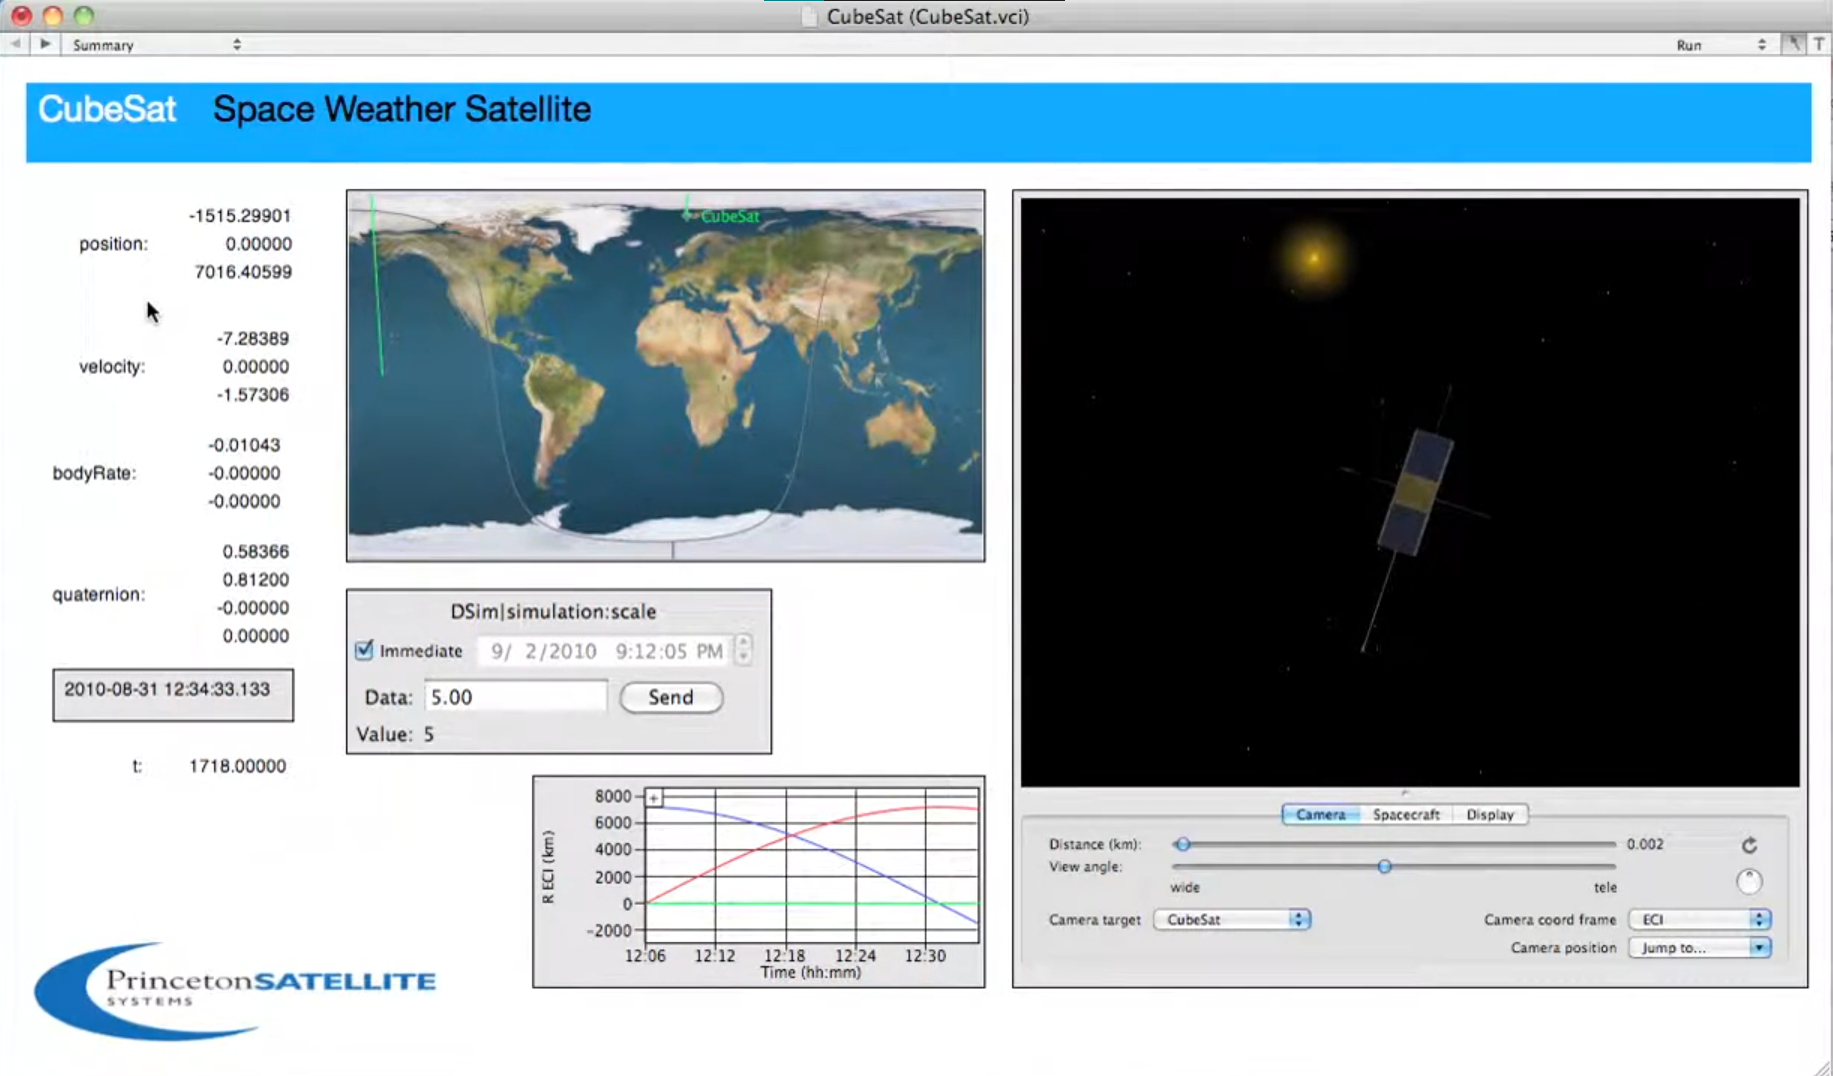
\includegraphics[width=0.75\textwidth]{Cubesat_Toolbox.png}
		\caption{Resumen de la dinámica orbital y de actitud del satélite en CubeSat Toolbox.}
		\label{fig:cube_Tool}
	\end{figure}
	
	\begin{figure}[H]
		\centering    
		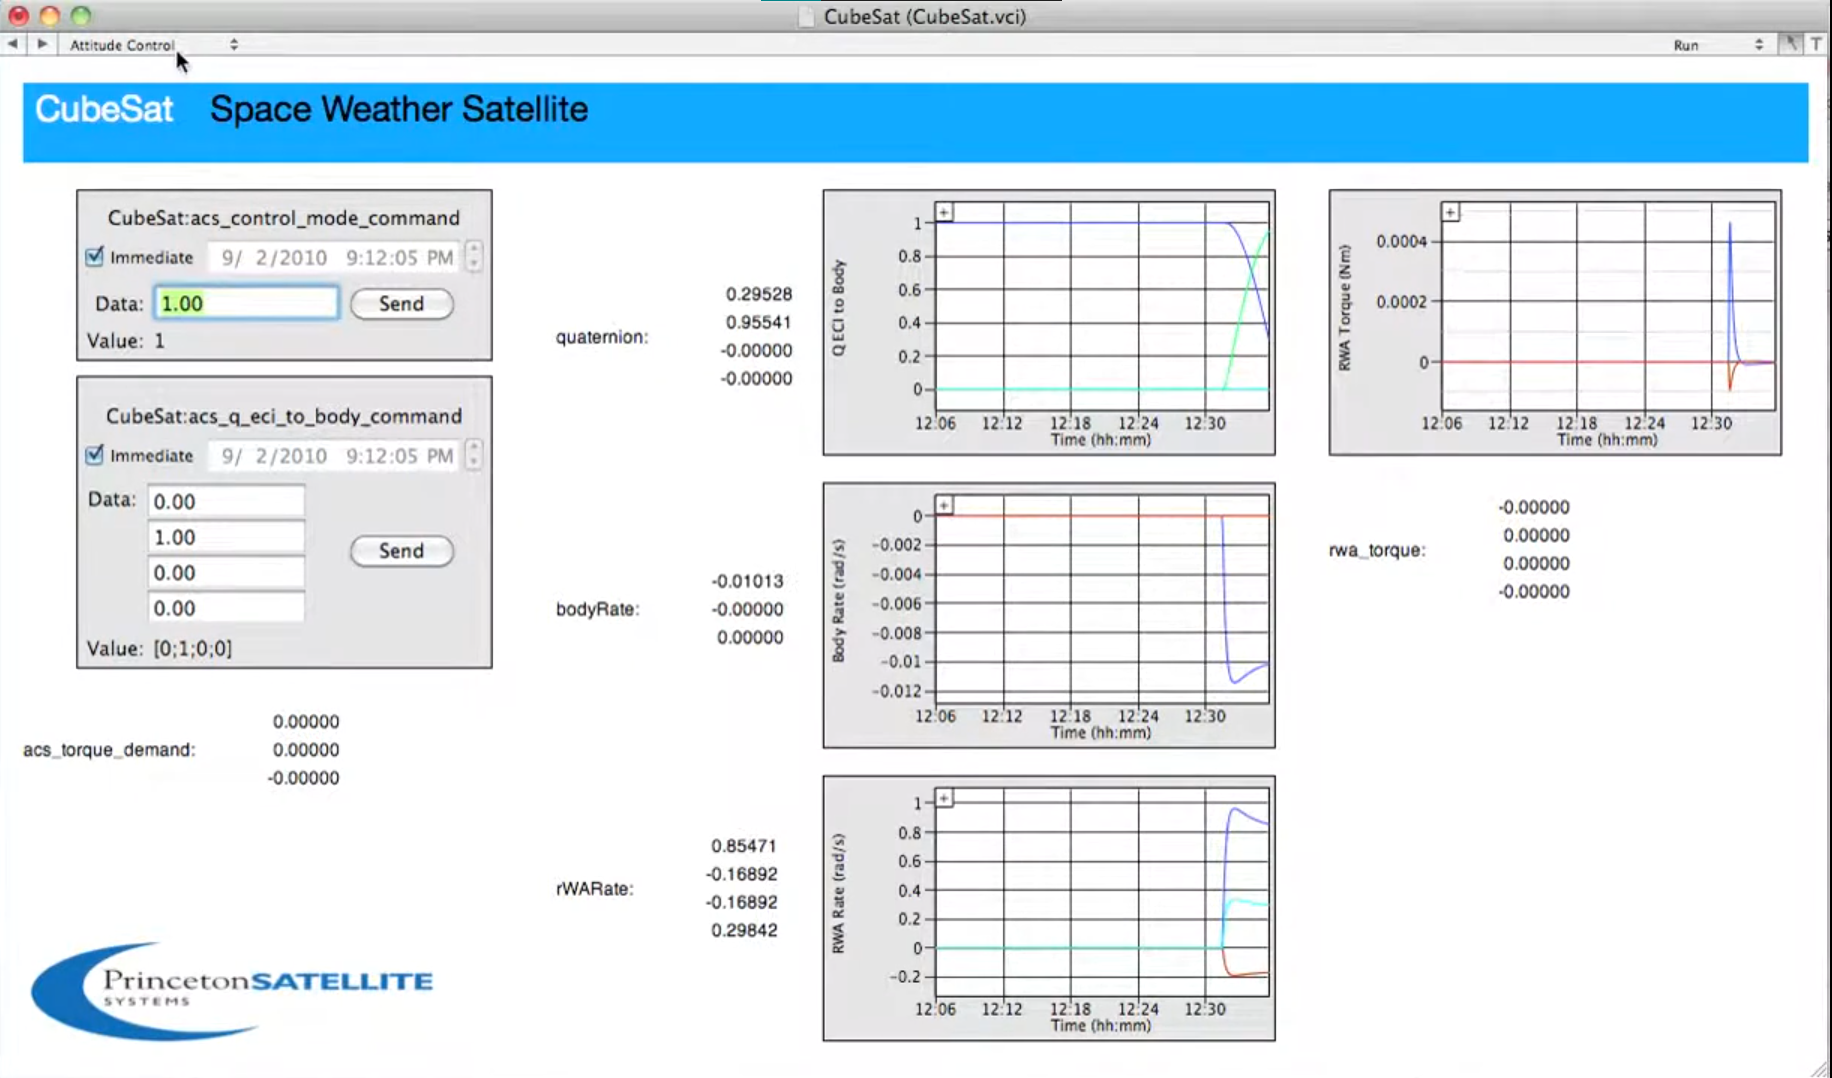
\includegraphics[width=0.75\textwidth]{Cubesat_Toolbox_2.png}
		\caption{Ventana de control del simulador de un CubeSat en CubeSat Toolbox.}
		\label{fig:cube_ctrl}
	\end{figure}
	
	\item \textit{Spacecraft Control Toolbox versión académica}: La edición académica de la caja de herramientas contiene gran parte del software profesional Spacecraft Control Toolbox, incluidas las herramientas CAD, las funciones de diseño de control y dinámica de actitud, la mecánica orbital y el módulo CubeSat. Además, incluye esquemas de apuntamiento según marcos de referencia LVLH, sun-nadir pointing y latitude/longitude, y también otorga los pointing budgets más relevantes como la exactitud de apuntamiento. Esta versión cuesta 3995 dólares su adquisición y presenta un breve tutorial en el canal de YouTube de Princeton.
	
	\item \textit{Spacecraft Control Toolbox versión profesional}: La edición profesional de Spacecraft Control Toolbox ofrece todo lo que hay en las versiones CubeSat y Academic, con la adición de herramientas avanzadas para la estimación de actitud y órbita, modelado de sensores y actuadores y análisis de subsistemas. Las aplicaciones de la caja de herramientas incluyen diseño de sistemas de control, simulación no lineal, análisis de órbitas y planificación de misiones, incluidas trayectorias interplanetarias, diseño y disposición de naves espaciales, estudios comerciales y visualización de actitudes y órbitas. La versión profesional cuesta 11995 dólares, siendo esta la más completa y a la vez más cara entre las tres mencionadas.
\end{itemize}


\subsection{Ansys Systems Tool Kit (STK)}

STK es una plataforma de software líder en el mercado diseñada para el modelado y análisis de sistemas complejos y sus interacciones en una variedad de dominios, incluyendo espacio, defensa y aplicaciones aeroespaciales. Esta herramienta proporciona una serie de capacidades avanzadas que permiten a los ingenieros, científicos y analistas modelar, simular y visualizar sistemas dinámicos de manera efectiva \cite{ref34}.

Es relevante ya que es capaz de modelar un satélite mediante su diseño 3D, mostrando gráficamente como este se propaga a través de la órbita. También es capaz de simular los cambios de actitud del satélite a través del tiempo y mostrar si efectivamente se está apuntando hacia la zona requerida de la tierra (exactitud de apuntamiento). En la Figura~\ref{fig:STK} se aprecia una imagen referencial de la simulación de un satélite en 3D y sus marcos de referencia cuerpo y LVLH. El costo de la licencia investigativa de este software es de alrededor de 4527 dólares por un año, que sería la versión útil para la realización del proyecto.

\begin{figure}[H]
	\centering    
	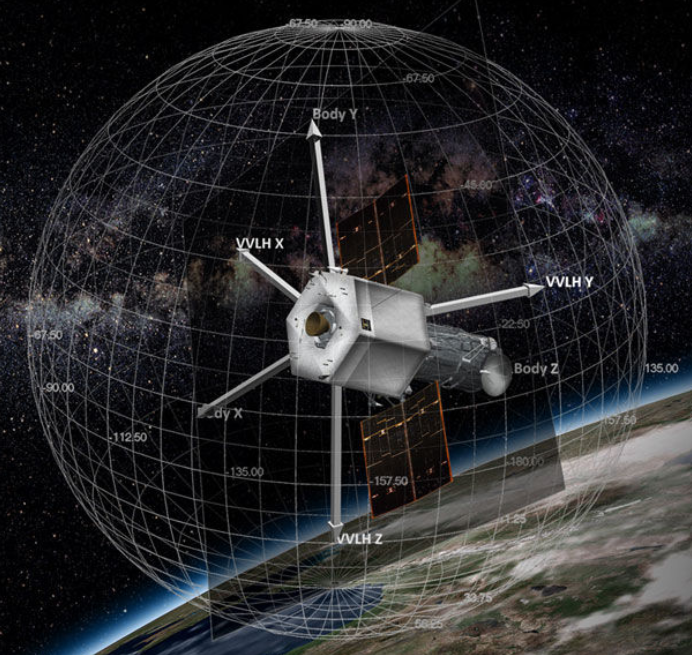
\includegraphics[width=0.4\textwidth]{STK.png}
	\caption{Imagen referencial de STK para simulación de un satélite.}
	\label{fig:STK}
\end{figure}
\subsection{Aerospace Blockset}

Dentro de este módulo en MATLAB, existen librerías capaces de modelar, simular y analizar CubeSats con facilidad \cite{ref19}. Algunas de las capacidades clave incluyen:

\begin{itemize}
	\item \textit{Modelado de CubeSats}:  El modelo de plantilla es un ejemplo listo para simular que contiene un bloque de vehículo CubeSat. MATLAB permite a los usuarios modelar CubeSat para proporcionar una opción de planificación de misión de alto nivel/creación rápida de prototipos para modelar y propagar rápidamente órbitas de satélites, un satélite a la vez. En este bloque se debe especificar el estado orbital inicial y modo de control de actitud (apuntamiento hacia el sol, nadir Tierra o personalizado), como se observa en la Figura~\ref{fig:blockset_1}.
	
	\begin{figure}[H]
		\centering    
		\includegraphics[width=0.7\textwidth]{blockset_1.png}
		\caption{Plantilla de Simulink para el diseño de un CubeSat.}
		\label{fig:blockset_1}
	\end{figure}
	
	\item Simulación de Misiones: El proyecto es un ejemplo listo para simular con visualización utilizando Simulink 3D Animation, como se muestra en la Figura~\ref{fig:blockset_2}jemplo utiliza un subsistema de modelo de vehículo por defecto, pero también se puede utilizar el modelo de CubeSat diseñado en el paso anterior. Con el módulo, es posible simular misiones completas de CubeSats, lo que incluye la evaluación de la trayectoria, la dinámica orbital con modelos de perturbaciones incluidas y las operaciones a bordo. Esto es esencial para prever el comportamiento del CubeSat en el espacio y optimizar su rendimiento.
	
	\begin{figure}[H]
		\centering    
		\includegraphics[width=0.9\textwidth]{blockset_2.png}
		\caption{Plantilla de Simulink para la modelación y simulación del CubeSat en base a la visualización en Simulink 3D.}
		\label{fig:blockset_2}
	\end{figure}	
	
	\item \textit{Proyecto utilizando \gls{MBSE} en CubeSat}: Es un ejemplo listo para simulación que muestra cómo modelar la arquitectura de una misión espacial con System Composer y Aerospace Blockset. El proyecto hace referencia al Proyecto de simulación CubeSat para reutilizar modelos de subsistema, luego agrega una capa de arquitectura System Composer, vincula los requisitos del sistema con los componentes de la arquitectura y verifica los requisitos de la misión de nivel superior con Simulink Test™. El proyecto visualiza los resultados utilizando Simulink 3D Animation, escenarios satelitales de Aerospace Toolbox y Mapping Toolbox™. Todo esto se muestra según los bloques mostrados en la Figura~\ref{fig:blockset_3}.
	
	\begin{figure}[H]
		\centering    
		\includegraphics[width=0.6\textwidth]{blockset_3.png}
		\caption{Visualización del MBSE de CubeSat.}
		\label{fig:blockset_3}
	\end{figure}	
	
	Mediante la última librería mencionada se puede obtener la observación terrestre de un CubeSat, además de visualizar los budgets de costo como lo es el precio, la masa, la potencia tanto peak como promedio y el tamaño. También presenta en una interfaz gráfica los errores de determinación de actitud y de apuntamiento, además de los torques ejercidos por los actuadores (sean modelados o por defecto dentro del programa), como se muestra en la Figura~\ref{fig:blockset_4}. Así, se puede visualizar el resultado como muestra la Figura~\ref{fig:blockset_5}.
	
	\begin{figure}[H]
		\centering    
		\includegraphics[width=0.6\textwidth]{blockset_4.png}
		\caption{Perfil de CubeSat según los SE envelopes configurables.}
		\label{fig:blockset_4}
	\end{figure}	
	
	\begin{figure}[H]
		\centering    
		\includegraphics[width=0.75\textwidth]{blockset_5.png}
		\caption{Simulación de apuntamiento de la Tierra hacia la estación terrestre.}
		\label{fig:blockset_5}
	\end{figure}	
\end{itemize}

\subsection{Valispace}

Valispace es una plataforma integral de ingeniería y gestión de proyectos diseñada para simplificar y optimizar el proceso de desarrollo de productos y sistemas, especialmente en industrias como la aeroespacial. La plataforma ofrece una variedad de herramientas y características poderosas que permiten a los equipos de ingeniería colaborar eficientemente, gestionar requisitos y parámetros críticos, y tomar decisiones informadas en tiempo real \cite{ref35}.

Las características claves son la gestión de datos en tiempo real, permitiendo el acceso en tiempo real y la colaboración de los miembros del equipo de ingeniería de forma actualizada. También permite a los equipos diseñar, analizar y optimizar sistemas de ingeniería complejos en base a requisitos que se imponen en el mismo programa al inicio del proyecto. Además, Valispace facilita el cálculo de parámetros críticos como costos, masa, potencia y tamaño, lo que es esencial en proyectos de ingeniería. Los resultados se pueden calcular y actualizar automáticamente a medida que se realizan cambios en el diseño.

\subsection{Basilisk}

El simulador Basilisk es un entorno de simulación avanzado, modular y extensible, desarrollado principalmente por el Laboratorio de Sistemas de Vehículos Espaciales de la Universidad de Colorado, Boulder. Su principal objetivo es facilitar la simulación de sistemas de naves espaciales, con un enfoque en la dinámica y el control de actitud. Este simulador ha sido ampliamente utilizado en investigaciones académicas y proyectos que requieren la modelación precisa de la dinámica y control de vehículos espaciales \cite{ref36}.

Una de las principales ventajas de Basilisk es su capacidad para simular sistemas multi-plataforma y multi-cuerpo, permitiendo la modelación de la dinámica orbital y de actitud de diversos cuerpos en el espacio. Esto incluye la simulación de perturbaciones ambientales, así como el comportamiento de subsistemas complejos como el \gls{ADCS}. Estas capacidades hacen que Basilisk sea especialmente útil para misiones que involucran satélites pequeños o CubeSats, donde las dinámicas precisas y los ajustes de actitud son críticos.

Otra de las fortalezas del simulador radica en su arquitectura modular. Cada subsistema —como los sensores, actuadores, o la dinámica orbital— está diseñado de manera independiente, lo que permite no solo la fácil personalización del código, sino también la posibilidad de integrar nuevos módulos o realizar simulaciones específicas de determinados componentes. Esta flexibilidad es clave para proyectos de investigación que requieren ajustes finos y configuraciones personalizadas.

El simulador también ofrece la capacidad de realizar simulaciones tanto en tiempo real como en tiempo no real, lo que resulta útil para diferentes tipos de aplicaciones. Las simulaciones en tiempo real permiten la implementación de pruebas de hardware-in-the-loop, mientras que las simulaciones en tiempo no real ofrecen mayor fidelidad para estudios más detallados.

\subsection{Resumen de los simuladores disponibles}

Para tener en claro si es posible el uso de algunos de estos softwares presentes en el estado del arte (SOA) en la suite de simulación, se toma en cuenta la Tabla~\ref{tab:sims}, en la cual, en base a criterio propios, se analiza cada opción y su viabilidad.

\begin{table}[ht]
	\centering
	\caption{Comparativa de software/simuladores para CubeSats.}
	\label{tab:sims}
	\begin{tabular}{|l|c|c|c|c|}
		\hline
		\textbf{Software/} & \textbf{Precio [USD]}  & \textbf{Dificultad} & \textbf{MoP de} & \textbf{SE envelopes} \\
		\textbf{simulador} &  &  & \textbf{apuntamiento} &  \\ \hline
		\textit{CubeSat}     & 495 + Matlab          & Media               & No presenta                & Potencia                \\ 
		\textit{Toolbox}     & & &  &            \\ \hline
		SCT                 & 3995 + Matlab         & Alta                & Exactitud   & Potencia          \\ 
		académico                & &  &  de apuntamiento & y masa          \\ \hline
		SCT               & 11995 + Matlab        & Alta                & Exactitud de & Potencia, \\
		profesional              &  &  &  apuntamiento/agilidad & masa y tamaño \\ \hline
		\textit{Aerospace}  & Matlab                & Muy             & Exactitud de   & Todos, con imposición \\
		\textit{Blockset}  &                 & alta            &  apuntamiento  & de requisitos \\ \hline
		Systems               & 4527 por año          & Media               & Exactitud de  & Potencia         \\ 
		ToolKit              & &                & apuntamiento/agilidad &          \\ \hline
		Valispace                    & 1295 por año          & Media               & No presenta                & Todos                  \\ \hline
		Basilisk & Gratis & Muy Alta & Configurable & Configurable \\ \hline
	\end{tabular}

\end{table}


Para el caso del precio, son accesibles las opciones de CubeSat Toolbox y Aerospace Blockset, ya que una suscripción de MATLAB cuesta alrededor de 275 USD por año para versión académica, la cual se presenta disponible en el marco de su uso dentro de la Universidad de Concepción como estudiante/académico. Se descarta la primera opción al no presentar un análisis de los MoP de apuntamiento. Otra razón para descartar su uso es que se presenta exclusivamente en MATLAB, siendo que la suite de simulación se pretende armar en Python, por lo que habría que reformular el código dentro de este lenguaje de programación. 

Por otro lado, el Aerospace Blockset se presenta como una buena opción, aunque sea un pack de herramientas disponibles en MATLAB. Si bien esta logra analizar al menos uno de los MoP de apuntamiento, su uso se basa en MBSE, el cual requiere de un manejo del Systems Engineering de medio a alto, escapándose en parte del conocimiento requerido para la optimización de los resultados en el simulador. Además, no presenta la opción de hacer lazo cerrado por fuera del software, por lo que la combinación de herramientas es bastante rígida.

Finalmente, Basilisk se muestra como una opcion interesante a considerar, ya que presenta ya simulado la dinamica orbital y de actitud considerando distinto hardware del \gls{ADCS}. Esta se toma en cuenta solo como una buena referencia, debido a su elevada curva de aprendizaje y a su documentación que puede ser demasiado técnica o incompleta para el tiempo acotado de trabajo. Además, aunque se pueden realizar simulaciones detalladas del sistema \gls{ADCS} y dinámicas orbitales, Basilisk no tiene un enfoque nativo en la optimización de sistemas, teniendo que configurar los parametros de rendimiento y costo para este uso.

Por lo tanto, de los simuladores que se pueden adquirir, sirven como una base para implementar de manera propia una suite de simulación con capacidad de optimización.
\section{Diseño de la suite de simulación}

\subsection{Marco general del simulador}

Para la construcción de la suite de simulación, se debe tener en cuenta tanto la dinámica orbital como la dinámica de actitud, para así tener conocimiento del posicionamiento y la velocidad del CubeSat a través del espacio, y de la actitud de este en su desplazamiento alrededor de la Tierra. Para ello se debe considerar los siguientes elementos como base:

\begin{itemize}
	\item \textbf{\textit{Propagación orbital}}: En primera instancia, el simulador busca conocer el posicionamiento del satélite alrededor de la Tierra, por lo que es necesario el uso de un propagador orbital adecuado capaz de entregar información sobre el vector posición y velocidad del satélite respecto a la Tierra. Además, se debe considerar las perturbaciones correspondientes para la altura del satélite analizado, que en este caso se acotará a órbitas bajas, con el objetivo de hacer el movimiento traslacional del satélite realista según las condiciones espaciales presentes.
	
	\item \textbf{\textit{Modelos orbitales}}: Los modelos orbitales son necesarios para obtener la orientación del CubeSat. Con ello se obtendrán las representaciones necesarias de los sensores en el marco de referencia inercial.
	
	\item \textbf{\textit{Sensores}}: Para determinar la actitud del satélite, se seleccionan sensores capaces de entregar información relevante sobre la inercia del satélite, el comportamiento físico del ambiente espacial o estrellas circundantes. Es relevante tanto para la estimación inicial como para el conocimiento de la actitud a través del tiempo y se simularan según los modelos orbitales analizados, teniendo en cuenta una rotación del marco de referencia inercial al marco de referencia del cuerpo y el ruido en la lectura de los componentes utilizados.
	
	\item \textbf{\textit{Algoritmos de estimación de actitud}}: Estos son necesarios para trabajar los vectores entregados por los sensores y los modelos orbitales. Con estos se obtienen los cuaterniones que representan las rotaciones del satélite a través del tiempo. Se busca utilizar el EKF para la estimación de los estados posteriores, además de una mitigación del ruido en la obtención de la orientación del satélite.
	
	\item \textbf{\textit{ Controladores y actuadores}}: Ya obtenidas la actitud del satélite a través del tiempo, se desea que el CubeSat apunte a una dirección en específico. Para ello se implementa el uso de un controlador capaz de realizar el control del satélite mediante la entrega del modelo dinámico y del actuador. Esto va de la mano con la selección del actuador a utilizar, para tener en cuenta las limitaciones de la acción de control al apuntar el satélite hacia la dirección deseada.
	
\end{itemize}

Teniendo en cuenta estos factores, la Figura~\ref{fig:bloq_gen} presenta un diagrama que resume la estructura de la suite de simulación, utilizada para obtener los resultados de los  MoP de apuntamiento y los SE envelopes correspondientes. En primer lugar, se obtiene el vector de estado $\vec{r}$ del CubeSat mediante el propagador orbital, seguido por el uso de modelos orbitales para calcular $\vec{V}_{ref}$, el vector en el sistema de referencia inercial. Simultáneamente, a través de la lectura de los sensores, se obtienen los vectores $\vec{V}_{obs}$ en el marco de referencia del cuerpo. Posteriormente, se realiza el cambio de sistema de referencia de $\vec{V}_{ref}$ a LVLH (como se explicará en las secciones siguientes), utilizando ambos vectores para la estimación del cuaternión $q$. Finalmente, se ejecuta la acción de control mediante el controlador seleccionado, considerando la restricción del torque $\tau$ ejercido por el actuador. En las próximas secciones se detallará el diseño y selección de cada componente de la suite de simulación.

\begin{figure}[h]
	\centering    
	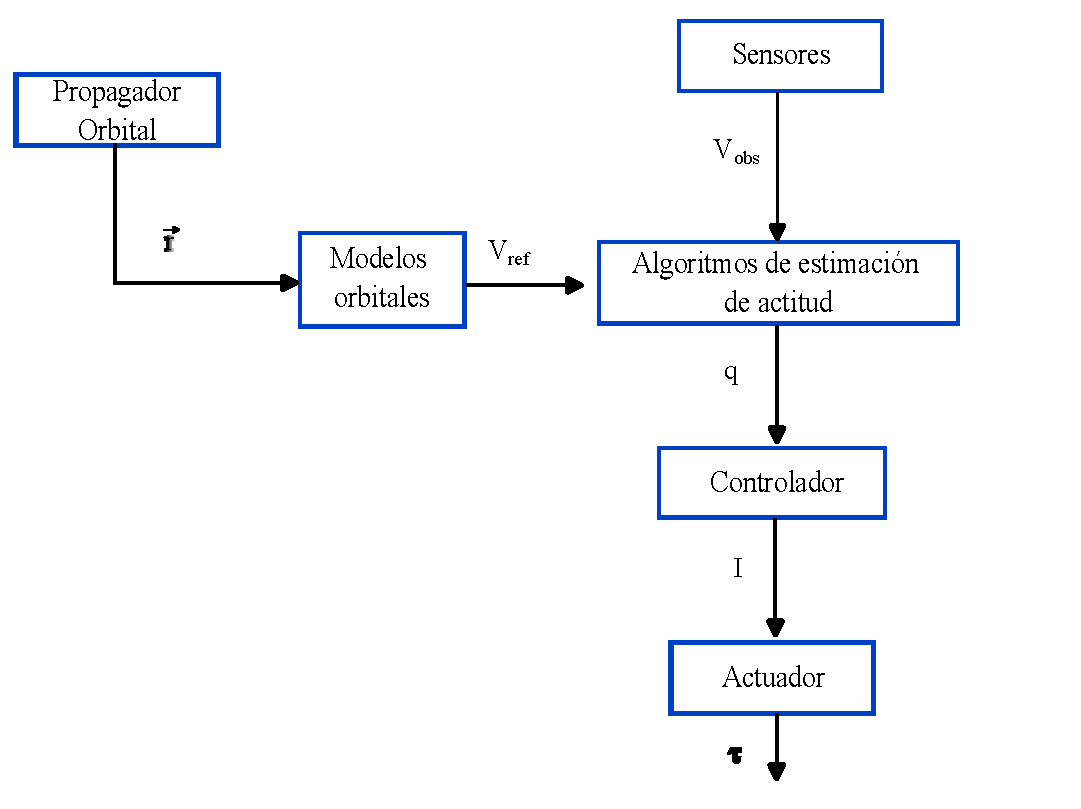
\includegraphics[width=0.65\textwidth]{bloques_generico.pdf}
	\caption{Esquema general de la base del simulador (Elaboración propia).}
	\label{fig:bloq_gen}
\end{figure}

\subsection{Propagador orbital}

Para la simulación de la dinámica orbital, se debe considerar la implementación de un propagador capaz de entregar la posición y velocidad del satélite respecto a la Tierra incluyendo las perturbaciones relevantes a baja altura. Para ello se proponen las siguientes opciones:

\textbf{\textit{Simplified General Perturbation 4 (SGP4) \cite{ref37}}}:Es un modelo matemático que se utiliza ampliamente para predecir la posición y velocidad de los satélites. Utiliza las ecuaciones de movimiento de dos cuerpos, que describen cómo un satélite se mueve bajo la influencia de la gravedad de la Tierra, y luego aplica una serie de perturbaciones para tener en cuenta factores como la forma no esférica de la Tierra, el arrastre atmosférico, la radiación solar y los efectos gravitacionales de la interacción con otros cuerpos como el Sol o la Luna. El SGP4 utiliza los Two Line Elements (TLE) como entrada, que es un formato estándar utilizado para describir la órbita de un satélite en dos líneas, en conjunto con la fecha de inicio y el tiempo de propagación, para después aplicar una serie de ecuaciones y algoritmos que calculan los elementos orbitales futuros del satélite en función del tiempo.

\textbf{\textit{FreeFlyer \cite{ref38}}}:Es un programa de simulación espacial diseñado para visualizar y modelar varios escenarios, incluyendo, pero no limitándose a la propagación y maniobras de naves espaciales, análisis de cobertura y contacto, análisis interplanetario y la generación de diversos recursos visuales. Es capaz de propagar el movimiento del satélite a través del tiempo e incluir perturbaciones como J2, arrastre atmosférico, efecto multi-cuerpo y radiación solar.

\textbf{\textit{Systems Tool Kit (STK) \cite{ref34}}}: Es una plataforma ampliamente utilizada en el ámbito tanto aeronáutico como espacial. El STK es un simulador de Ansys utilizado para el diseño, planificación y simulación de misiones. Una de sus herramientas es la propagación del satélite a través del tiempo con una interfaz gráfica, incluyendo todas las perturbaciones presentes en el espacio.

Se descartan las opciones de los softwares FreeFlyer y STK debido a su alto costo monetario para la implementación del simulador solo para su uso en la dinámica orbital. Por lo tanto, se elige el SGP4 no solo por ser una opción gratuita, sino porque es fácil de implementar a cualquier satélite que se conozca su TLE. Esta entrega el movimiento traslacional del satélite a través del tiempo considerando las perturbaciones más importantes a bajas alturas.

Para analizar el funcionamiento del propagador, se utilizó como ejemplo un TLE del SUCHAI-3 obtenido de CelesTrak y se propagó durante un día tomando como fecha de inicio 1 de noviembre del 2023 a las 12 del mediodía. Se observa en la Figura~\ref{fig:pos} y ~\ref{fig:vel} la posición y la velocidad respecto al marco de referencia ECI obtenido en Python a través de la librería SGP4.

\begin{figure*}[h]
	\centering
	\begin{subfigure}[t]{0.68\textwidth}
		\centering{%
			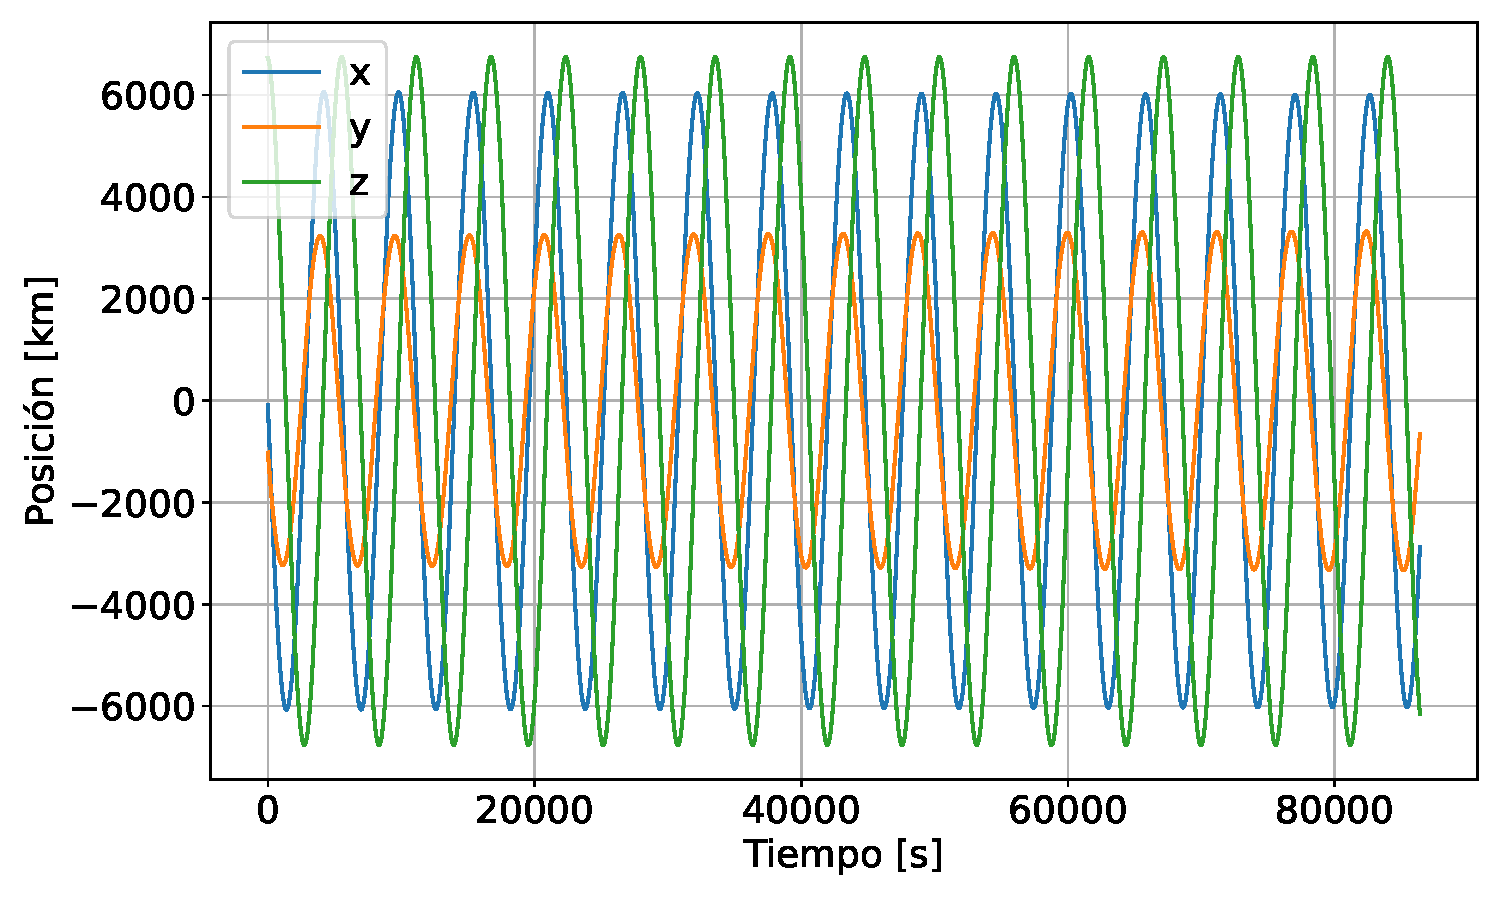
\includegraphics[width=\textwidth]{pos.pdf}
		}%
		\subcaption{Posición del satélite.\label{fig:pos}}
	\end{subfigure}
	\begin{subfigure}[t]{0.68\textwidth}
		\centering{%
			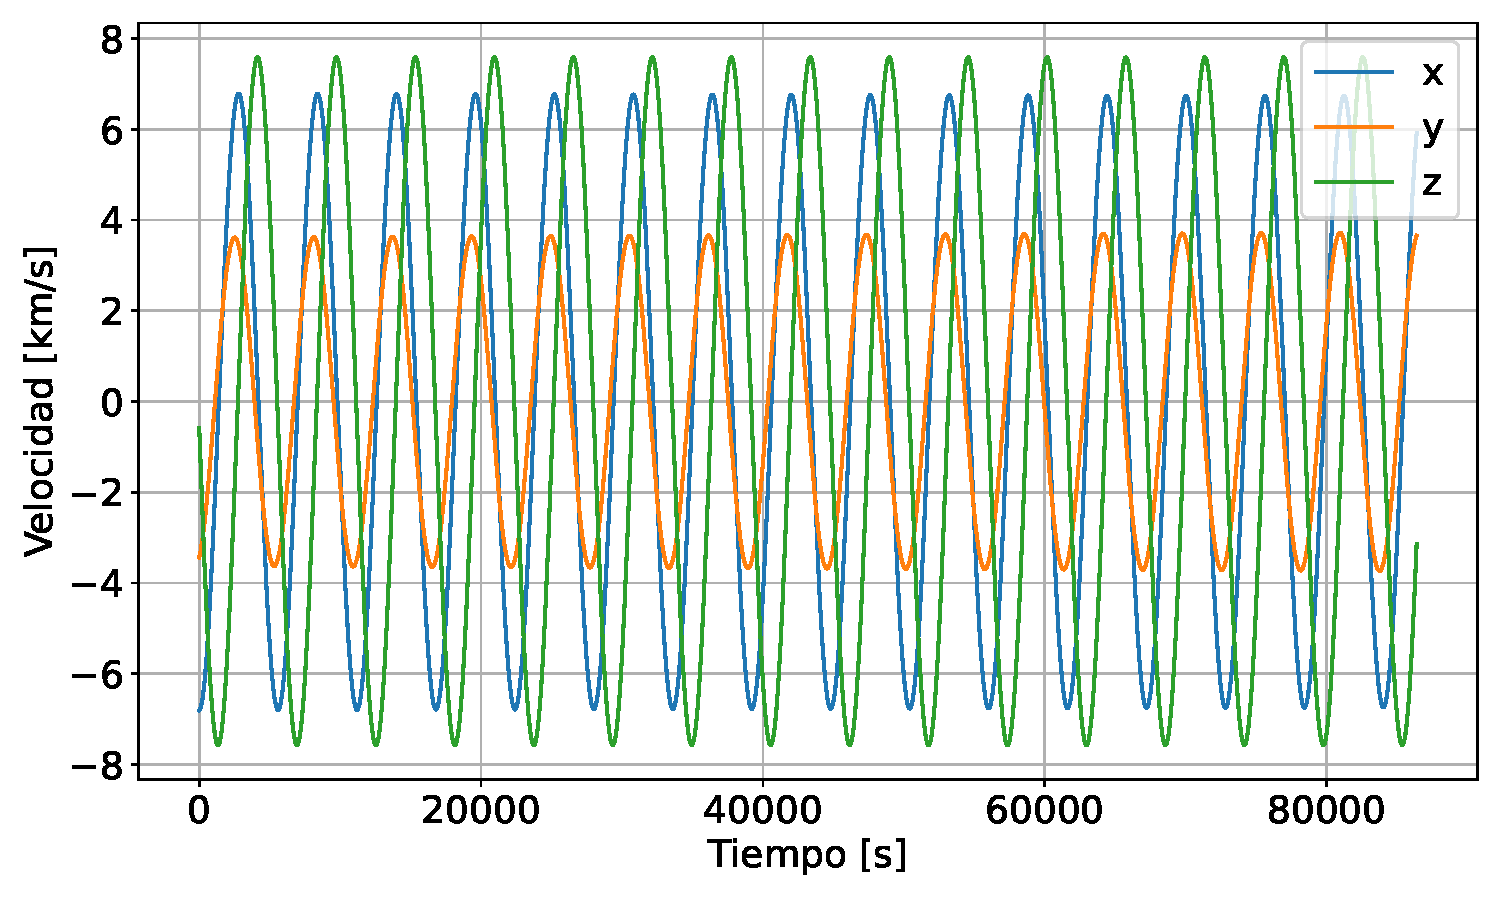
\includegraphics[width=\textwidth]{vel.pdf}
		}%
		\subcaption{Velocidad del satélite.\label{fig:vel}}
	\end{subfigure}
	\caption{Propagación del SUCHAI-3 durante un día con fecha de inicio 01/11/23.}\label{fig:pos-vel}
\end{figure*}


\subsection{Modelos orbitales y sistemas de referencia}

Para la obtención de la actitud del satélite se requieren conocer dos vectores respecto al marco de referencia Local Vertical Local Horizontal (LVLH) o también llamado orbital.  Para ello se conocerán en primera instancia los modelos del sol y del campo geomagnético terrestre para la obtención de los vectores en el marco de referencia inercial (ECI), para luego rotarlos al sistema LVLH. Posteriormente se obtendrán los vectores de observación, que se generan en base a los modelos mencionados aplicando otra rotación desde orbital al cuerpo, que representan los vectores medidos por los sensores.

\subsubsection{Vector sol}

El modelo se basa principalmente en el movimiento del sol respecto al sistema de referencia ECI. Lo primero a tener en cuenta es la anomalía media del sol, la cual se calcula según muestra la Ecuación~\ref{eq:M_sun} y consiste en el ángulo medido desde el perigeo, que describe la posición del Sol en su trayectoria orbital y depende puramente del tiempo \cite{ref15}.

\begin{equation}
	M_{\text{sun}} = M_{\text{sunEpoch}} + n_{\text{sun}}JD_{2000} = 357.528^\circ +   0.9856003^\circ \cdot JD_{2000}
	\label{eq:M_sun}
\end{equation}

En la ecuación anterior, $M_{\text{sunEpoch}}$ es el valor conocido de la anomalía media del Sol para el 1 de enero de 2000 al mediodía en UTC y $n_{\text{sun}}$ es el movimiento medio del Sol, el cual también es un valor conocido. La anomalía media del Sol puede entonces calcularse para cualquier $JD_{2000}$, que se refiere a la fecha juliana respecto al año 2000. A partir de la anomalía media, se puede calcular la longitud de la eclíptica $\lambda_{\text{sun}}$ según la Ecuación~\ref{eq:lambda_sun}, que representa la posición del Sol en el plano orbital bidimensional en el marco ECI.

\begin{equation}
	\lambda_{\text{sun}} = 280.461^\circ + 0.9856474^\circ \cdot JD_{2000} + 1.915^\circ \sin(M_{\text{sun}}) + 0.020^\circ \sin(2 M_{\text{sun}})
	\label{eq:lambda_sun}
\end{equation}

Para determinar completamente la posición del Sol en el marco ECI, se requiere conocimiento de la inclinación de la órbita desde el plano orbital bidimensional. Este parámetro se llama oblicuidad del plano de la eclíptica y se define en la Ecuacion~\ref{eq:eps_sun}

\begin{equation}
	\epsilon = 23.4393^\circ + 0.0000004^\circ \cdot JD_{2000}
	\label{eq:eps_sun}
\end{equation}

La posición del Sol en el marco ECI ahora se puede calcular como un vector unitario con las componentes representadas en la Ecuación~\ref{eq:x_sun}, ~\ref{eq:y_sun} y ~\ref{eq:z_sun}.

\begin{equation}
	X_{\text{sun}} = \cos(\lambda_{\text{sun}})
	\label{eq:x_sun}
\end{equation}

\begin{equation}
	Y_{\text{sun}} = \cos(\epsilon) \sin(\lambda_{\text{sun}})
	\label{eq:y_sun}
\end{equation}

\begin{equation}
	Z_{\text{sun}} = \sin(\epsilon) \sin(\lambda_{\text{sun}})
	\label{eq:z_sun}
\end{equation}

Este modelo del vector sol se observa en la Figura~\ref{fig:ss}, en la cual se simula propagando por un año desde el 01 de noviembre del 2023, el cual en días julianos corresponde al día 2460250. Se observa en dicha gráfica un comportamiento oscilatorio, notándose un ciclo entero del movimiento del sol recién al término de la simulación.

\begin{figure}[h]
	\centering    
	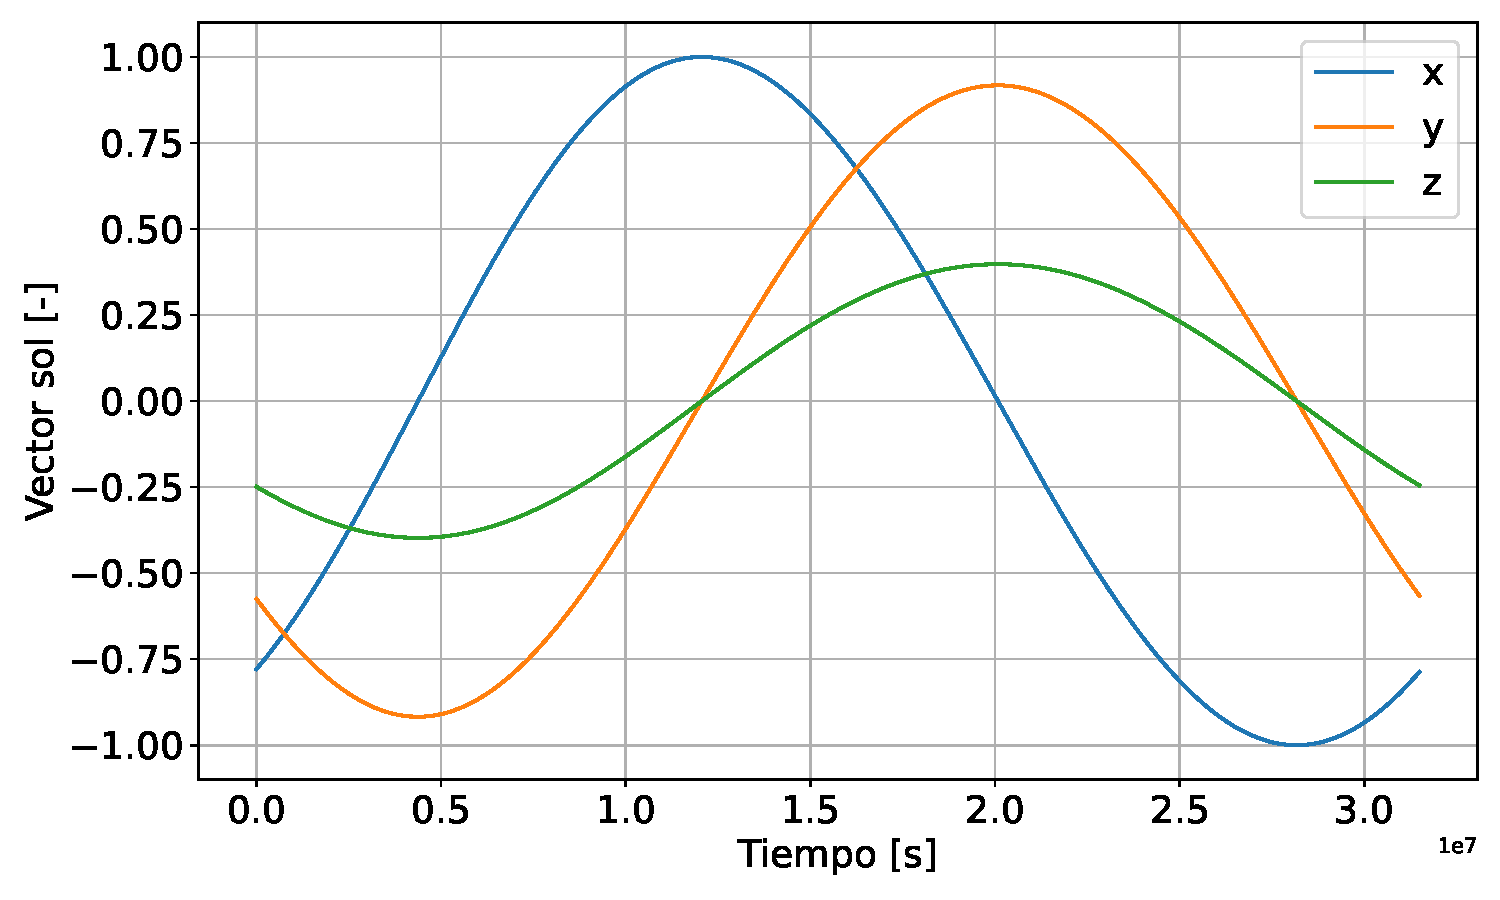
\includegraphics[width=0.65\textwidth]{ss.pdf}
	\caption{Vector sol en sus tres componentes simulados durante un año (Elaboración propia).}
	\label{fig:ss}
\end{figure}


\subsubsection{Fuerzas geomagnéticas de la Tierra}

Para el modelamiento de las fuerzas geomagnéticas de la tierra en distintas posiciones de la órbita de un satélite se requiere el uso del International Geomagnetic Reference Field (IGRF). Este campo de referencia consiste en un conjunto de coeficientes armónicos esféricos que pueden introducirse en un modelo matemático, para así describir la porción a gran escala y variable en el tiempo del campo magnético interno de la Tierra entre las épocas 1900 d.C. y el presente. El IGRF utilizado para la realización del simulador es el de decima tercera generación y se ha derivado de observaciones registradas por satélites, observatorios terrestres y estudios magnéticos \cite{ref39}.

El IGRF describe el principal campo geomagnético $B(r, \theta, \varphi, t)$ que es producido por fuentes internas, principalmente dentro del núcleo de la Tierra. El IGRF es válido dentro y alrededor de la superficie de la Tierra, donde el campo geomagnético principal puede describirse como el gradiente de un potencial escalar, $B = -\nabla V$, y la función potencial $V(r, \theta, \varphi, t)$ se representa en la Ecuación~\ref{eq:potencial} como una expansión en serie finita en términos de coeficientes armónicos esféricos, $g_n^m, h_n^m$, también conocidos como coeficientes de Gauss:

\begin{equation}
	V(r, \theta, \varphi, t) = a \sum_{n=1}^{N} \sum_{m=0}^{n} \left( \frac{a}{r} \right)^{n+1} 
	\left[ g_n^m(t) \cos(m \varphi) + h_n^m(t) \sin(m \varphi) \right] P_n^m(\cos(\theta))
	\label{eq:potencial}
\end{equation}

Aquí, $r, \theta, \varphi$ se refieren a coordenadas en un sistema de coordenadas esféricas geocéntricas o geodésicas, siendo $r$ la distancia radial desde el centro de la Tierra o la altura desde su superficie dependiendo de si son geocéntricas o geodésicas respectivamente, y $\theta, \varphi$ son la co-latitud y longitud geocéntricas respectivamente. 

Las $P_n^m (\cos(\theta))$ son funciones de Legendre asociadas seminormalizadas de Schmidt de grado $n$ y orden $m$. El parámetro $N$ especifica el grado máximo de expansión armónica esférica y se eligió que fuera 10 hasta la época 1995 inclusive, después de lo cual aumenta a 13. Por otro lado, los coeficientes de Gauss cambian en el tiempo y se proporcionan en unidades de nanoTesla (nT) en IGRF-13 en intervalos de época de 5 años. La dependencia temporal de estos parámetros se modela como lineal por partes y viene dada por:

\begin{equation}
	g_n^m (t) = g_n^m (T_t) + (t - T_t) \dot{g}_n^m (T_t)
\end{equation}

\begin{equation}
	h_n^m (t) = h_n^m (T_t) + (t - T_t) \dot{h}_n^m (T_t)
\end{equation}

Donde $g_n^m (T_t)$, $h_n^m (T_t)$ son los coeficientes de Gauss en la época $T_t$, que precede inmediatamente al tiempo $t$. Las épocas del modelo en IGRF-13 se proporcionan en múltiplos exactos de 5 años comenzando en 1900 y terminando en 2020, de modo que $T_t < t < T_t+5$. Para $T_t < 2020$, los parámetros $\dot{g}_n^m (T_t)$, $\dot{h}_n^m (T_t)$ representan la aproximación lineal al cambio en los coeficientes de Gauss durante el intervalo de 5 años que abarca $[T_t, T_t+5]$. Pueden calcularse en unidades de nanoTesla por año (nT/año) como:

\begin{equation}
	\dot{g}_n^m (T_t) = \frac{1}{5} \left( g_n^m (T_t+5) - g_n^m (T_t) \right)
\end{equation}

\begin{equation}
	\dot{h}_n^m (T_t) = \frac{1}{5} \left( h_n^m (T_t+5) - h_n^m (T_t) \right)
\end{equation}

Este procedimiento en Python viene entregado por la National Centers for Environmental Information (NCEI) \cite{ref40} bajo el nombre de paquete \texttt{py.igrf} y se implementa en el simulador para el conocimiento de las fuerzas magnéticas ejercidas sobre la Tierra. Se requiere para el modelo insertar como parámetros de entrada las coordenadas geodésicas $(r, \theta, \varphi)$ en conjunto con el año de análisis, para así obtener siete salidas (declinación [°], inclinación [°], intensidad horizontal [nT], componente norte [nT], componente este [nT], componente vertical [nT] e intensidad total [nT]), siendo las componentes 4, 5 y 6 las fuerzas magnéticas en el marco de referencia ECI.

Para conocer las coordenadas geodésicas y simular un receptor GPS sin ruido dentro del satélite, se hizo un cambio de sistema de referencia desde ECI a geodésicas. Utilizando la librería Skyfield de Python y conociendo la posición en la cual está el satélite respecto a la Tierra gracias al propagador SGP4, se conocen las coordenadas GPS en cada instante del movimiento traslacional del satélite. Para analizar el funcionamiento del modelo IGRF entregado en Python, se utilizó los vectores posición y velocidad de la sección 5.3.1 correspondiente al SUCHAI-3 para hacer el cambio de sistema ECI a geodésicas, obteniendo en la Figura~\ref{fig:bb} las fuerzas magnéticas del satélite a través del tiempo.


\begin{figure}[h]
	\centering    
	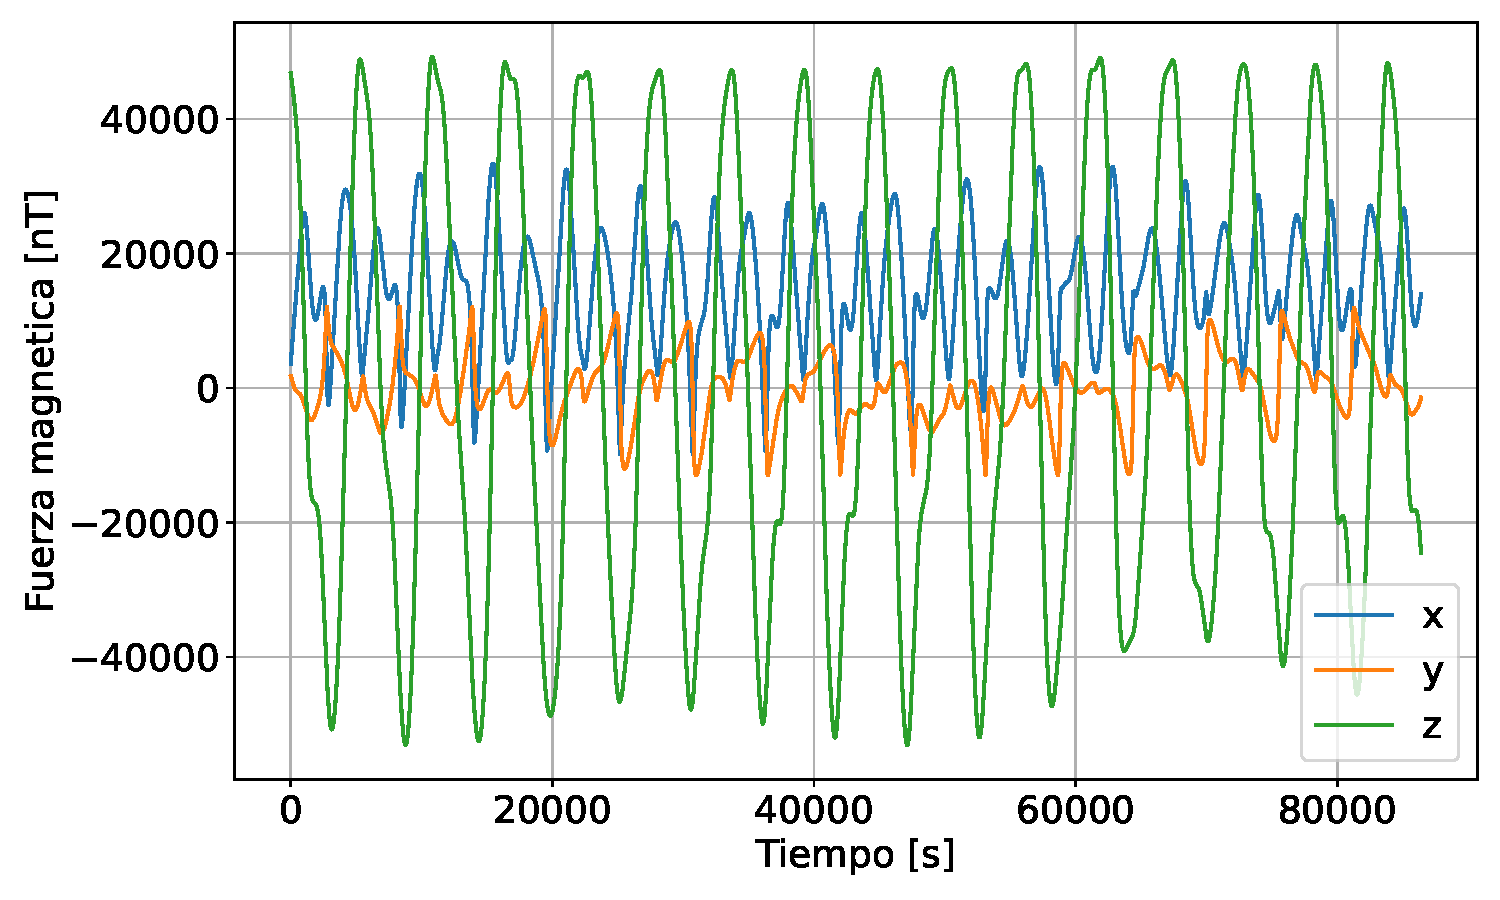
\includegraphics[width=0.65\textwidth]{bb.pdf}
	\caption{Componentes de las fuerzas magnéticas respecto a ECI que afectan al SUCHAI-3 con fecha inicial 01/11/2023 (Elaboración propia).}
	\label{fig:bb}
\end{figure}

\subsubsection{Cambios en los sistemas de referencia y vectores de observación}

Ya obtenidos los vectores sol y las fuerzas magnéticas en ECI, se aplica una matriz de rotación desde ECI a LVLH utilizando los vectores posición $\vec{P}$ y velocidad $\vec{V}$ calculados en la Sección 4.2 proveniente del SGP4. Dicha matriz de rotación se representa de la siguiente manera \cite{ref9}:

\[
	\vec{Z_O} = \frac{\vec{P}}{\|\vec{P}\|} \quad 	\vec{X_O} = \frac{\vec{V} \times \vec{Z_O}}{\|\vec{V} \times \vec{Z_O}\|} \quad 	\vec{Y_O} = \vec{Z_O} \times \vec{X_O} 
\]

\[
	R_{\text{ECI}}^O = 
	\begin{bmatrix}
		\vec{X_O}^T &
		\vec{Y_O}^T &
		\vec{Z_O}^T
	\end{bmatrix}
\]

Utilizando esta matriz, en conjunto con el cuaternión inicial estimado, el cual se representa como $R_{\text{ECI}}^{\text{body}}$, se obtiene la matriz de rotación que relaciona el marco de referencia del cuerpo con el orbital, mediante la siguiente relación:

\[
	R_O^{\text{body}} = (R_{\text{ECI}}^{O})^T \cdot R_{\text{ECI}}^{\text{body}}
\]

Mediante esta matriz de rotación, la cual puede ser transformada a un cuaternión $q_O^{\text{body}}$, se puede aplicar el control que será analizado en secciones posteriores utilizando una condición inicial en el sistema de referencia adecuado. Para la obtención de los vectores sol y las fuerzas magnéticas en el marco de referencia del cuerpo, se genera el cuaternión entre los marcos de referencia a medida que se estima en el siguiente paso de tiempo. Es relevante reconocer que se utilizan las mismas relaciones de rotación para la obtención de los vectores $B_O$ y $\vec{v}_{\text{sun}, O}$ usando los cuaterniones $q_{\text{ECI}}^{O}$.

\[
	(q_O^{\text{body}})^{-1} = [-q_0, -q_1, -q_2, q_3]
\]

\[
	B_{\text{body}} = (q_O^{\text{body}})^{-1} \cdot B_O \cdot q_O^{\text{body}}
\]

\[
	\vec{v}_{\text{sun, body}} = (q_O^{\text{body}})^{-1} \cdot \vec{v}_{\text{sun, O}} \cdot q_O^{\text{body}}
\]

\subsection{Algoritmos de estimación y control satelital}

Ya obtenidos los vectores de referencia y de observación, se puede estimar la orientación (cuaterniones) y la velocidad angular del satélite a través del tiempo. Para ello se estima la actitud actual mediante mediciones y métodos matemáticos, para posteriormente definir una acción de control que logrará apuntar hacia la actitud objetivo (sistema de referencia LVLH) utilizando un sistema de control automático.

\subsubsection{Conversión representación de rotación y EKF}

Para la realizacion de la suite de simulación, se hace entrega de un cuaternión inicial tanto para el modelo que representa las mediciones llamada 'real' y otra condición inicial 'estimada' para cada paso del EKF. Además, para el análisis de resultados, se utilizan los ángulos de Euler para una mayor comprensión conceptual y física de los cambios de orientación ocurridos en el satélite. En el Anexo \ref{ap:Z3} se presentan dichas conversiones matemáticas.

Se utilizó el Filtro de Kalman Extendido (EKF) de forma recursiva para estimar la actitud del satélite, tomando como referencia inicial el estado estimado. Este filtro fue implementado para su uso tanto con los magnetorquers como con las ruedas de reacción, utilizando modelos dinámicos lineales discretos. En cada caso, se ajustaron las matrices de estado A y de control B, mientras que la matriz de salida C se construyó a partir de las mediciones simuladas del magnetómetro y el sensor solar.

En cuanto a la matriz C, dado que depende de las mediciones del magnetómetro, las cuales varían con el tiempo, dicha matriz también cambia a lo largo de la simulación. Al intentar linealizar el control en la siguiente sección, las matrices A y B no varían con el tiempo, pero la matriz de salida sí, lo que dio origen al término "Semiextendido". Para más detalles sobre el diseño del filtro de Kalman "Semiextendido", se puede consultar el Anexo \ref{ap:Z4}.

\subsubsection{Controladores y actuadores}

Se ha optado por utilizar el controlador Proporcional-Derivativo (PD) debido a su simplicidad y a su capacidad para orientar el satélite hacia una posición específica. Adicionalmente, se ha simulado el controlador Linear Quadratic Regulator (LQR) para obtener una matriz de ganancia que garantice un control estable en ambos actuadores simulados. Sin embargo, es importante destacar que se logró un control estable únicamente con el controlador PD aplicado al magnetorquer; por lo tanto, el uso de este controlador se presenta solo para este actuador.

Para utilizar un controlador, es fundamental comprender la linealización del sistema, un proceso útil para simplificar modelos no lineales como las Ecuaciones~\ref{eq:cin_omega} y~\ref{eq:vect_dot} y facilitar el diseño de estrategias de control. Este proceso se basa en la aproximación de Taylor \cite{ref42}, que consiste en linealizar las ecuaciones alrededor de un punto de equilibrio.

Esto implica calcular las derivadas parciales de las funciones de estado con respecto a las variables de estado y de control. Las matrices resultantes, $A = \frac{\partial f(x,u)}{\partial x}$ y $B = \frac{\partial f(x,u)}{\partial u}$, representan la dinámica linealizada del sistema, generando así el modelo espacio estado (EE) mostrado a continuación.

\[
	\dot{x} = A x + B u
\]
Es importante destacar que la linealización proporciona una descripción local del comportamiento del sistema alrededor del punto de equilibrio, y por lo tanto, la validez de este enfoque depende de la proximidad del estado actual del sistema al punto de equilibrio.

Además, se optan por el magnetorquer\cite{ref14} y la rueda de reacción\cite{ref41} como actuadores, debido a la documentación encontrada sobre su utilización y su uso mayoritario en nanosatélites. Para conocer el álgebra y las consideraciones del diseño del control lineal a mayor detalle para cada actuador, se recomienda revisar el Anexo \ref{ap:Z5} y \ref{ap:Z6} respectivamente. 

\underline{Magnetorquer}

El punto de equilibrio para el caso del modelo dinamico con magnetorquer se muestra a continuación, cuyos valores representan que no existe diferencia de orientación entre los marcos de referencia del cuerpo y orbital, además de lograr que se minimice tanto la acción de control como la velocidad angular \cite{ref14}.

\[
	q_{\text{co}} = [0, 0, 0, 1] \quad	u = [0, 0, 0] \quad	\omega_{\text{co}} = [0, 0, 0]
\]



Los torques de control en sus tres componentes se representan en las Ecuaciones~\ref{eq:MT_x},~\ref{eq:MT_y} y~\ref{eq:MT_z}.


\begin{equation}
	\tau_{x,\text{mt}} = \left( \frac{b_x m_z - b_z m_x}{\|b\|} \right) b_z - \left( \frac{b_y m_x - b_x m_y}{\|b\|} \right) b_y
	\label{eq:MT_x}
\end{equation}

\begin{equation}
	\tau_{y,\text{mt}} = -\left( \frac{b_z m_y - b_y m_z}{\|b\|} \right) b_z + \left( \frac{b_y m_x - b_x m_y}{\|b\|} \right) b_x
	\label{eq:MT_y}
\end{equation}

\begin{equation}
	\tau_{z,\text{mt}} = \left( \frac{b_z m_y - b_y m_z}{\|b\|} \right) b_y - \left( \frac{b_x m_z - b_z m_x}{\|b\|} \right) b_x
	\label{eq:MT_z}
\end{equation}

Donde b son las fuerzas magnéticas en el marco de referencia del cuerpo y m es el momento dipolar del magnetorquer.

Evaluando los valores deseados de $q_{\text{co}}$ y $\omega_{\text{co}}$ en las matrices $A$ y $B$ mencionadas en el Anexo \ref{ap:Z5}, se obtiene:

\[
	A = \begin{bmatrix}
		0 & 0 & 0 & 0.5 & 0 & 0 \\
		0 & 0 & 0 & 0 & 0.5 & 0 \\
		0 & 0 & 0 & 0 & 0 & 0.5 \\
		6\omega_{(0,o)}^2 [I_z - I_y] & 0 & 0 & 0 & 0 & 0 \\
		0 & 6\omega_{(0,o)}^2 [I_z - I_x] & 0 & 0 & 0 & \frac{\omega_{(0,o)} (I_x - I_y)}{I_z} - I_z \omega_{(0,o)} \\
		0 & 0 & 0 & 0 & \frac{\omega_{(0,o)} (I_x - I_z)}{I_y} + I_y \omega_{(0,o)} & 0
	\end{bmatrix}
\]

\[
	\bar{B} = \begin{bmatrix}
		0 & 0 & 0 \\
		0 & 0 & 0 \\
		0 & 0 & 0 \\
		\frac{-b_z^2 - b_y^2}{\|b\| I_x} & \frac{b_x b_y}{\|b\| I_y} & \frac{b_x b_z}{\|b\| I_z} \\
		\frac{b_x b_y}{\|b\| I_x} & \frac{-b_z^2 - b_x^2}{\|b\| I_y} & \frac{b_y b_z}{\|b\| I_z} \\
		\frac{b_x b_z}{\|b\| I_x} & \frac{b_y b_z}{\|b\| I_y} & \frac{-b_y^2 - b_x^2}{\|b\| I_z}
	\end{bmatrix}
\]

Debido a que aun cuando se implementa una linealización en el equilibrio, las fuerzas magnéticas de la Tierra siguen variando, se debe obtener una matriz de cotrol representativa para su uso en el modelo espacio estado:

\[
	B = \frac{1}{T} \int_{t_0}^{t_{0+T}} \bar{B}(t) \, dt
\]

Para el caso del controlador LQR, con las matrices A y B y las matrices Q y R entregadas por el diseñador del control, se logra obtener la matriz de ganancia K y ejercer el control en el modelo dinámico.

Por otro lado, para el controlador PD, se debe representar el modelo espacio estado de la siguiente manera:

\[
	\dot{x} = \hat{A} x
\]

Con: 

\[
	\hat{A} = A + BK
\]

\[
	K = \begin{bmatrix}
		K_{p,x} & 0 & 0 & K_{d,x} & 0 & 0 \\
		0 & K_{p,y} & 0 & 0 & K_{d,y} & 0 \\
		0 & 0 & K_{p,z} & 0 & 0 & K_{d,z} \\
		
	\end{bmatrix}
\]

Las constantes \(K_p\) y \(K_d\) son las constantes proporcionales y derivativas del controlador, y desempeñan un papel crucial en la determinación de la estabilidad del sistema. Estas constantes se ajustan de manera que los valores propios de la matriz \(A + BK\) sean negativos, lo que garantiza la estabilidad del sistema en lazo cerrado.

Los valores propios negativos son indicativos de que el sistema es asintóticamente estable, lo que significa que las respuestas transitorias del sistema convergen hacia el estado de equilibrio deseado sin oscilaciones ni divergencias. En otras palabras, los valores propios negativos aseguran que el sistema retorne a su estado de equilibrio después de cualquier perturbación, lo que es fundamental para el funcionamiento adecuado del sistema de control, con un rendimiento estable y robusto \cite{ref43}.

\underline{Ruedas de reacción}

El punto de equilibrio para el caso del modelo dinamico con rueda de reacción se muestra a continuación, cuyos valores representan que no existe diferencia de orientación entre los marcos de referencia del cuerpo y orbital, además de lograr que se minimice tanto la acción de control como la velocidad angular del satélite y de cada rueda de reacción simulada (en este caso tres) \cite{ref41}.

\[
q_{\text{co}} = [0, 0, 0, 1] \quad u = [0, 0, 0] \quad 	\omega_{\text{co}} = [0, 0, 0] \quad 	\omega_{\text{rw}} = [0, 0, 0]
\]



Los torques de control son ejercidos por cada rueda de reacción de manera directa, siendo colocados en los tres ejes de referencia del marco de referencia del cuerpo del CubeSat por simplicidad. De esta manera, la rueda modelada en el eje x se representa mediante $\tau_{x, \text{rw}}$. Mismo caso para $\tau_{y, \text{rw}}$ y $\tau_{z, \text{rw}}$

Como se observa para los puntos de equilibrio, en este caso son nueves estados que se reemplazan en la matriz de estado A y B obtenida en el Anexo \ref{ap:Z6}, generando como resultado las siguientes matrices simplificadas:

\[
A_{11} = A_{13}
\begin{bmatrix}
	0 & 0 & 0 \\
	0 & 0 & 0 \\
	0 & 0 & 0 \\
\end{bmatrix} \quad
A_{12} = 
\begin{bmatrix}
	0.5 & 0 & 0 \\
	0 & 0.5 & 0 \\
	0 & 0 & 0.5 \\
\end{bmatrix}
\]

\[
A_{21} = 
\begin{bmatrix}
	 6 \omega_{0,o}^2 \left[I_z - I_y\right]  & 0 & 0 \\
	0 & 6 \omega_{0,o}^2 \left[I_z - I_x\right] + \frac{2 \omega_{0,o}^2 \left(J_x - J_z\right)}{J_y - I_{s1}}
	 & 0 \\
	0 & 0 &  -\frac{2 \omega_{0,o}^2 \left(J_x - J_y\right)}{J_z - I_{s2}}
	 \\
\end{bmatrix}
\]

\[
A_{31} = 
\begin{bmatrix}
	6 \omega_{0,o}^2 \left[I_z - I_y\right]  & 0 & 0 \\
	0 & 6 \omega_{0,o}^2 \left[I_z - I_x\right] - \frac{2 \omega_{0,o}^2 \left(J_x - J_z\right)}{J_y - I_{s1}}
	& 0 \\
	0 & 0 &  \frac{2 \omega_{0,o}^2 \left(J_x - J_y\right)}{J_z - I_{s2}}
	\\
\end{bmatrix}
\]

\[
A_{22} = -A_{32} = 
\begin{bmatrix}
	0  & 0 & 0 \\
	0  & 0 & \frac{\omega_{0,o} \left(J_x - J_z\right)}{J_y - I_{s1}} + \omega_{0,o} \\
	0 & \frac{\omega_{0,o} \left(J_x - J_y\right)}{J_z - I_{s2}} - \omega_{0,o} & 0	\\
\end{bmatrix}
\]

\[
A_{23} = -A_{33} = 
\begin{bmatrix}
	0 & 0 & 0 \\
	0 & 0 & -\frac{\omega_{0,o} I_{s2}}{J_y - I_{s1}}
	 \\
	0 & -\frac{\omega_{0,o} I_{s1}}{J_z - I_{s2}}
	 & 0 \\
\end{bmatrix}
\]

\[
A =
\begin{bmatrix}
	A_{11} & A_{12} & A_{13} \\
	A_{21} & A_{22} & A_{23} \\
	A_{31} & A_{32} & A_{33}
\end{bmatrix}
\]

\[
B =
\begin{bmatrix}
	0 & 0 & 0 \\
	0 & 0 & 0 \\
	0 & 0 & 0 \\
	\frac{1}{J_{x}-I_{s0}} & 0 & 0 \\
	0 & \frac{1}{J_{y}-I_{s1}} & 0 \\
	0 & 0 & \frac{1}{J_{z}-I_{s2}} \\
	\frac{1}{I_{s0}} - \frac{1}{J_{x}-I_{s0}} & 0 & 0 \\
	0 & \frac{1}{I_{s1}} - \frac{1}{J_{y}-I_{s1}} & 0 \\
	0 & 0 & \frac{1}{I_{s2}} - \frac{1}{J_{z}-I_{s2}} \\
\end{bmatrix}
\]

Una vez obtenidas las matrices A y B, dado que no hay vectores externos que varíen en el tiempo, como ocurre en el caso del magnetorquer, es posible utilizar un controlador LQR para guiar el sistema hacia el punto de equilibrio. Para ello, se debe diseñar el controlador seleccionando adecuadamente las matrices de ponderación Q y R, las cuales permiten ajustar el compromiso entre el rendimiento y el esfuerzo de control.

Es importante señalar que para ambos actuadores, la acción de control u se determina utilizando el vector de estado estimado, lo que permite aplicar torques realistas basados en las estimaciones obtenidas a través del Filtro de Kalman Extendido (EKF). Además, el estado 'real' es aquel que simulará las mediciones de los sensores, mientras que el 'estimado' sera el que se utiliza en cada paso de tiempo del EKF.

\subsection{Suite de simulación completa}

Ya tomadas las decisiones y generados los modelos dinámicos, se hace un resumen de las subsecciones mencionadas anteriormente:

\begin{itemize}
	\item \textbf{\textit{Uso del propagador SGP4 para la simulación de la dinámica orbital}}: Se eligió este debido a que presenta disponibilidad en el lenguaje de programación Python, además de ser de libre acceso y modela las perturbaciones necesarias en LEO a través del tiempo. Los demás propagadores como FreeFlyer y STK mencionados no son de libre acceso (tienen un alto costo monetario) y pueden no tener una conexión directa con las demás herramientas que se implementaran dentro del diseño del ADCS.
	
	\item \textbf{\textit{Modelos orbitales y sensores por utilizar}}: En el caso de los modelos orbitales, se logra implementar los modelos de la fuerza geomagnética y del vector sol con éxito. Debido a ello, se simula el magnetómetro y el sensor de sol, debido a que se obtienen los vectores de observación a través de un cambio en el sistema de referencia de 'cuerpo' a 'orbital', además de la implementación del ruido característico del componente físico. Finalmente, el giroscopio aporta con la actualización del cambio angular en el CubeSat, obteniendo las velocidades angulares a través del tiempo.
	
	\item\textbf{\textit{ Algoritmo de determinación de actitud seleccionado}}: Para la estimación inicial se elige un valor cercano a la condición inicial del modelo. Para obtener las estimaciones del estado a través del tiempo, se implementa el uso del metodo recursivo utilizando el filtro de kalman extendido (EKF).
	
	\item \textbf{\textit{Actuadores y controladores por utilizar}}: Se simularán magnetorquers y ruedas de reacción para el control de actitud en el simulador, ya que son los más comunes en nanosatélites. En ambos casos, se implementará el controlador Linear Quadratic Regulator (LQR), debido a su capacidad para ejercer un control estable sobre las matrices de estado A y de control 	B, utilizando matrices de ponderación Q y R adecuadamente diseñadas. Particularmente, para los magnetorquers también se utilizará un controlador Proporcional-Derivativo (PD) junto al LQR. Esto se debe a que la dinámica de actitud del satélite puede representarse mediante un cuaternión (componente proporcional) y la velocidad angular (componente derivativo), lo que es suficiente para orientar el satélite hacia una dirección deseada.
\end{itemize}

El esquema de la suite de simulación puede verse en la Figura~\ref{fig:suite}. En este diagrama, se muestra que el satélite primero debe determinar su posición y velocidad en la órbita. Para lograrlo, el propagador recibe parámetros de entrada como el TLE del satélite, una fecha de simulación y un tiempo de propagación. A continuación, el vector de posición se convierte a coordenadas GPS para calcular la fuerza magnética, mientras que la fecha en formato JD2000, representada en el diagrama como t, se utiliza para determinar el vector solar. Ambos vectores, que están en el sistema de referencia ECI, se rotan al marco de referencia orbital utilizando los vectores de posición r y velocidad v, como se describe en la Sección xxx.

Por otro lado, el vector de estado estimado $x_{k}$ se utiliza tanto en el controlador como en el filtro de Kalman. En el controlador, se obtiene la matriz de ganancia K, lo que permite determinar la acción de control estimada, que luego es utilizada tanto en el modelo como en el filtro de Kalman.

En el diagrama, los bloques azules representan el flujo de control para las estimaciones, mientras que los bloques rojos corresponden a los vectores de estado reales para simular las mediciones. En ambos casos, los vectores magnético y solar se rotan al sistema de referencia del cuerpo (body frame) para generar las mediciones reales y estimadas del magnetómetro y el sensor solar. Estas mediciones se comparan dentro del filtro de Kalman para obtener el vector de salida. Con esto, se completa un paso de tiempo y el proceso continúa al siguiente.

\begin{figure}[H]
	\centering    
	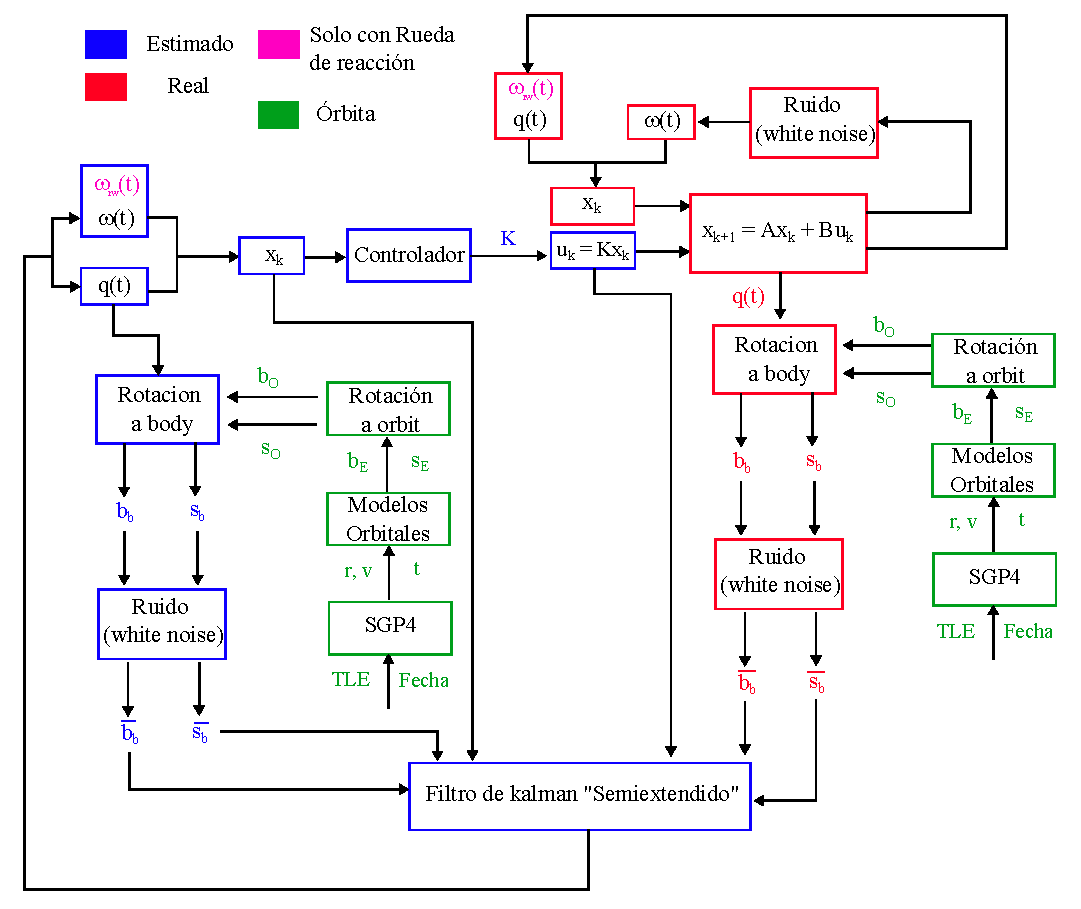
\includegraphics[width=0.9\textwidth]{suite.pdf}
	\caption{Diagrama de la suite de simulación completa (Elaboración propia).}
	\label{fig:suite}
\end{figure}
\section{Verificación de la suite de simulación}

En este capítulo se verán resultados en base a la elección de parámetros y datos de un CubeSat operativo, para obtener los MoP de apuntamiento con sus respectivos costos según los niveles de componentes físicos impuestos dentro de la simulación. Para ello, se define la cuantificación de los MoP de apuntamiento, se entregan los parámetros orbitales y se observan los valores obtenidos.

\subsection{Cuantificación de los MoP de apuntamiento}

Para lograr una capacidad de apuntamiento óptima, se debe considerar los MoP de apuntamiento. El apuntamiento se define como la capacidad que tiene el CubeSat para orientar la carga útil hacia un objetivo en específico, el cual, para este proyecto, será la tierra al imponer misiones del tipo observación terrestre. Teniendo esto en cuenta, existen índices de rendimiento con los cuales se verifica si este apuntamiento del satélite fue un éxito o un fracaso. Estos fueron revisados y descritos cualitativamente en \cite{ref6}, y debido a una revisión bibliográfica más extensa en libros sobre diseño de ADCS, se corrigieron y se cuantificaron, quedando como se muestra a continuación:

\underline{Exactitud de apuntamiento \cite{ref5,ref7}}

Es el índice con mayor relevancia dentro de las misiones de observación terrestre y de apuntamiento en general. Se refiere al error absoluto de apuntamiento del satélite, por lo que es la capacidad del CubeSat de mantener y controlar su orientación hacia una sección especifica de la Tierra. Esta se mide en termino de grados sexagesimales [°] o radianes [rad] y se notará dicho valor como la resta entre la orientación deseada del CubeSat y la posición obtenida mediante el ADCS, sabiendo que existen posibles errores de determinación de actitud o de actuadores que no puedan ejercer el torque requerido.

\underline{Jitter \cite{ref5,ref9,ref10}}

El Jitter en la línea de visión (LoS, por sus siglas en inglés) de la nave espacial se define como las vibraciones mecánicas sinusoidales de pequeña amplitud que ocurren debido a las interacciones dinámicas causadas por dispositivos mecánicos vibratorios montados en la nave espacial o dentro del instrumento (s) de carga útil y que aparecen a frecuencias en o por encima del ancho de banda del Attitude Control System (ACS) del satélite, desde unos pocos Hz hasta cientos de Hz, y que perturban indeseablemente el apuntamiento de la línea de visión de la carga útil. 

Para visualizar este problema, se debe revisar si existen en las sinusoidales alrededor del eje de equilibrio a controlar en los ángulos de Euler, leves perturbaciones asemejadas al ruido, que representan la inestabilidad del satélite al tomar diferentes orientaciones pequeñas en bajos periodos de tiempo, que hacen que la cámara sea vea “empañada”. Para representar dicho problema, se considera la densidad espectral de potencia como una medida de cuantificación del jitter, el cual se obtendrá una vez fijado un filtro pasa alto de hasta una frecuencia adecuada (generalmente 10 [Hz]) aplicada a la respuesta obtenida. Se observará un alto nivel de jitter si existe un valor de la densidad espectral de potencia mayor, al consumir más energía en dicho rango de frecuencias.


\underline{Agilidad \cite{ref5, ref11}}

Se refiere a lograr una maniobra de actitud mínima, el cual es una combinación de apuntar al objetivo (sección de la Tierra) en el menor tiempo posible a través de una maniobra de giro. En otras palabras, se busca que el CubeSat intercepte al objetivo lo más rápido posible y mantenga la orientación en una exactitud de apuntamiento aceptable dentro de los requerimientos.

Para cuantificar este índice, se hará uso del parámetro del tiempo de asentamiento (Settling Time), el cual especifica el tiempo permitido para recuperarse de maniobras o perturbaciones. Si existe un tiempo de asentamiento menor en alguna comparación de dos ADCS, sería más ágil aquel que presente un menor tiempo de asentamiento, comparándolo a través de una gráfica de velocidad angular respecto al tiempo, asumiendo una banda de asentamiento adecuada.

\underline{Drift \cite{ref5}}

Se refiere a cuánto puede desviarse un vehículo con el tiempo. Este parámetro es crucial cuando se necesita mantener una dirección específica y se deben hacer correcciones solo ocasionalmente para evitar que el vehículo se desvíe significativamente de su curso deseado. Representado mediante ángulos por hora [°/hr].

Para el caso de este análisis de la suite de simulación, se consideraron solo las tres primeras. El Drift solo se menciona, pero no se cuantifica en este trabajo.

\subsection{Condiciones y parámetros de simulación}

Para obtener resultados de rendimiento, se utilizaron los datos de TLE del SUCHAI-3 con fecha de inicio del 01 de noviembre del 2023, que son las mismas condiciones iniciales utilizadas en el Capítulo 4 para visualizar el SGP4 y los modelos orbitales en ECI (IGRF y vector sol). Se debe tener en cuenta que estas condiciones, en conjunto con otros parámetros son dados para todos los niveles de sensores y actuadores impuestos dentro de la suite de simulación, y sirven para tener un parámetro comparativo entre los componentes físicos del ADCS.

En la Tabla~\ref{tab:parametros} se muestran los valores de los parámetros recién mencionados utilizados en la simulación, que son basados en literatura \cite{ref14,ref41,ref44} o por elaboración propia. Cabe mencionar que $q_i$ y $\omega_i$ representan la orientación y velocidad angular inicial real.

\begin{table}[h!]
	\centering
	\caption{Parámetros del sistema}
	\begin{tabular}{|c|c|}
		\hline
		\textbf{Parámetro} & \textbf{Valor} \\
		\hline
		$[I_x, I_y, I_z] \ [kg \cdot m^2]$ & $[0.037, 0.036, 0.036]$ \\
		\hline		
		$[I_{s0}, I_{s1}, I_{s2}] \ [kg \cdot m^2]$ & $[0.005, 0.005, 0.004]$ \\
		\hline
		$[b_0, b_1, b_2] \ [m]$ & $[0.05, 0.05, 0.015]$ \\
		\hline		
		$\omega_{0,0} \ [rad/s]$ & $0.00163$ \\
		\hline
		$T_{\text{prop}} \ [s]$ & $345718 \ \text{[s]} \ (60 \ \text{órbitas})$ \\
		\hline
		$q_i \ [-]$ & $\left[ 0.0789, 0.0941, 0.0789, 0.9893 \right]$ \\
		\hline
		$\omega_i \ [rad/s]$ & $[0.0001, 0.0001, 0.0001]$ \\
		\hline
		$[\omega_{s0}, \omega_{s1}, \omega_{s2}] \ [rad/s]$ & $[0.00001, 0.00001, 0.00001]$ \\
		\hline
		$P_{i, \text{MT}}$ & $\text{diag}(0.25, 0.25, 0.25, 0.01, 0.01, 0.01)$ \\
		\hline
		$P_{i, \text{RW}}$ & $\text{diag}(P_{i, \text{MT}}, 0.001, 0.001, 0.001)$ \\
		\hline
	\end{tabular}

	\label{tab:parametros}
\end{table}

Además, con el objetivo de visualizar en el simulador el rendimiento de apuntamiento y su costo asociado, se decide agrupar los componentes físico en niveles según el COTS disponible en CubeSat~\cite{ref45}. Esto se hace debido a que existen una variedad considerable de componentes capaces de ser usado en este tipo de nanosatélites, al ser de poco costo tanto energético como monetario. Caracterizar todos estos se escapa de los objetivos del trabajo, ya que su consideración genera un análisis extenso e innecesario respecto a la obtención de los costos en base a los SE envelopes. Por ello, se presenta en la Tabla~\ref{tab:niveles} los componentes COTS seleccionados en conjunto con su proveedor para analizar tanto el rendimiento (MoP de apuntamiento) como el costo utilizado por cada uno de ellos. Mas detalles de cada uno de los sensores y actuadores elegidos en el Anexo \ref{ap:Z7}.

\begin{table}[h!]
	\centering
	\caption{Componentes clasificados por nivel de rendimiento}
	\begin{tabular}{|c|c|c|c|}
		\hline
		\textbf{Componente}   & \textbf{Nivel bajo} & \textbf{Nivel medio} & \textbf{Nivel alto} \\ 
		\hline
		\textbf{Giroscopio}   & CRH03 - 200  & CRH03 - 010  & NSGY-001   \\
		& (Silicon Sensing  & (Silicon Sensing & (NewSpace \\
		& Systems) & Systems) & Systems) \\
		\hline
		\textbf{Magnetómetro} & Fluxgate Magnetometer & MM200-1 & MM200-2  \\
		& FGM-A-75 & (AAC Clyde Space) & (AAC Clyde Space) \\
		& (ZARM Technik) & & \\
		\hline
		\textbf{Sun Sensor}   & CSS-01, CSS-02  & MSS-01 & FSS  \\
		& (Space Micro)   & (Space Micro) & (Bradford Space) \\
		\hline
		\textbf{Magnetorquer} & MT0.5-1 & NCTR-M012 & MT15-1 \\
		& (ZARM Technik) & (NewSpace Systems) & (ZARM Technik) \\
		\hline
		\textbf{Rueda de reacción} & RWP500 & RW1  & RW4  \\
		& (Blue Canyon & (Blue Canyon & (Blue Canyon \\
		& Technologies) & Technologies) & Technologies) \\
		\hline
	\end{tabular}
	\label{tab:niveles}
\end{table}


Es relevante mencionar que en el Anexo \ref{ap:Z8} se muestra un ejemplo a detalle sobre la obtención de los MoP de apuntamiento, siendo estos los pasos a seguir para los casos de estudio que se mencionarán en las siguientes secciones.

\subsection{Resultados suite de simulación}

En esta sección se presentarán análisis respecto a los resultados obtenidos utilizando los parámetros de la sección anterior. Se compararan los diferentes niveles de sensores y actuadores, los tipos de actuadores y los controladores utilizados para conocer la performance y costo de cada caso.

\subsubsection{Resultados tipos de actuadores}

A continuación, se presenta un análisis sobre el uso de los magnetorquers y las ruedas de reacción, destacando sus diferencias en cuanto a la performance de apuntamiento y el costo asociado.

En la Figura~\ref{fig:MT_RW_nivel2}, se muestran los ángulos de Euler a lo largo del tiempo utilizando sensores y actuadores de nivel medio (nivel 2). A la izquierda se observa el control ejercido por las ruedas de reacción, mientras que a la derecha, el control realizado por los magnetorquers. La Tabla~\ref{tab:RW_MT_nivel2} resume los resultados de la norma de los MoP de apuntamiento, junto con la diferencia en el consumo de potencia y la masa entre ambos tipos de actuadores.

La gráfica revela que las ruedas de reacción son capaces de generar torques de mayor magnitud, lo que permite alcanzar más rápidamente la orientación deseada en comparación con los magnetorquers. En ambos casos, se observa un comportamiento cíclico del ruido una vez que la orientación se estabiliza cerca de cero, lo cual se debe a la repetición de vectores de posición similares en cada órbita. Esto provoca que el campo magnético terrestre ejerza una fuerza de magnitud constante sobre el CubeSat, la cual es medida por el magnetómetro.

\begin{figure}[H]
	\centering    
	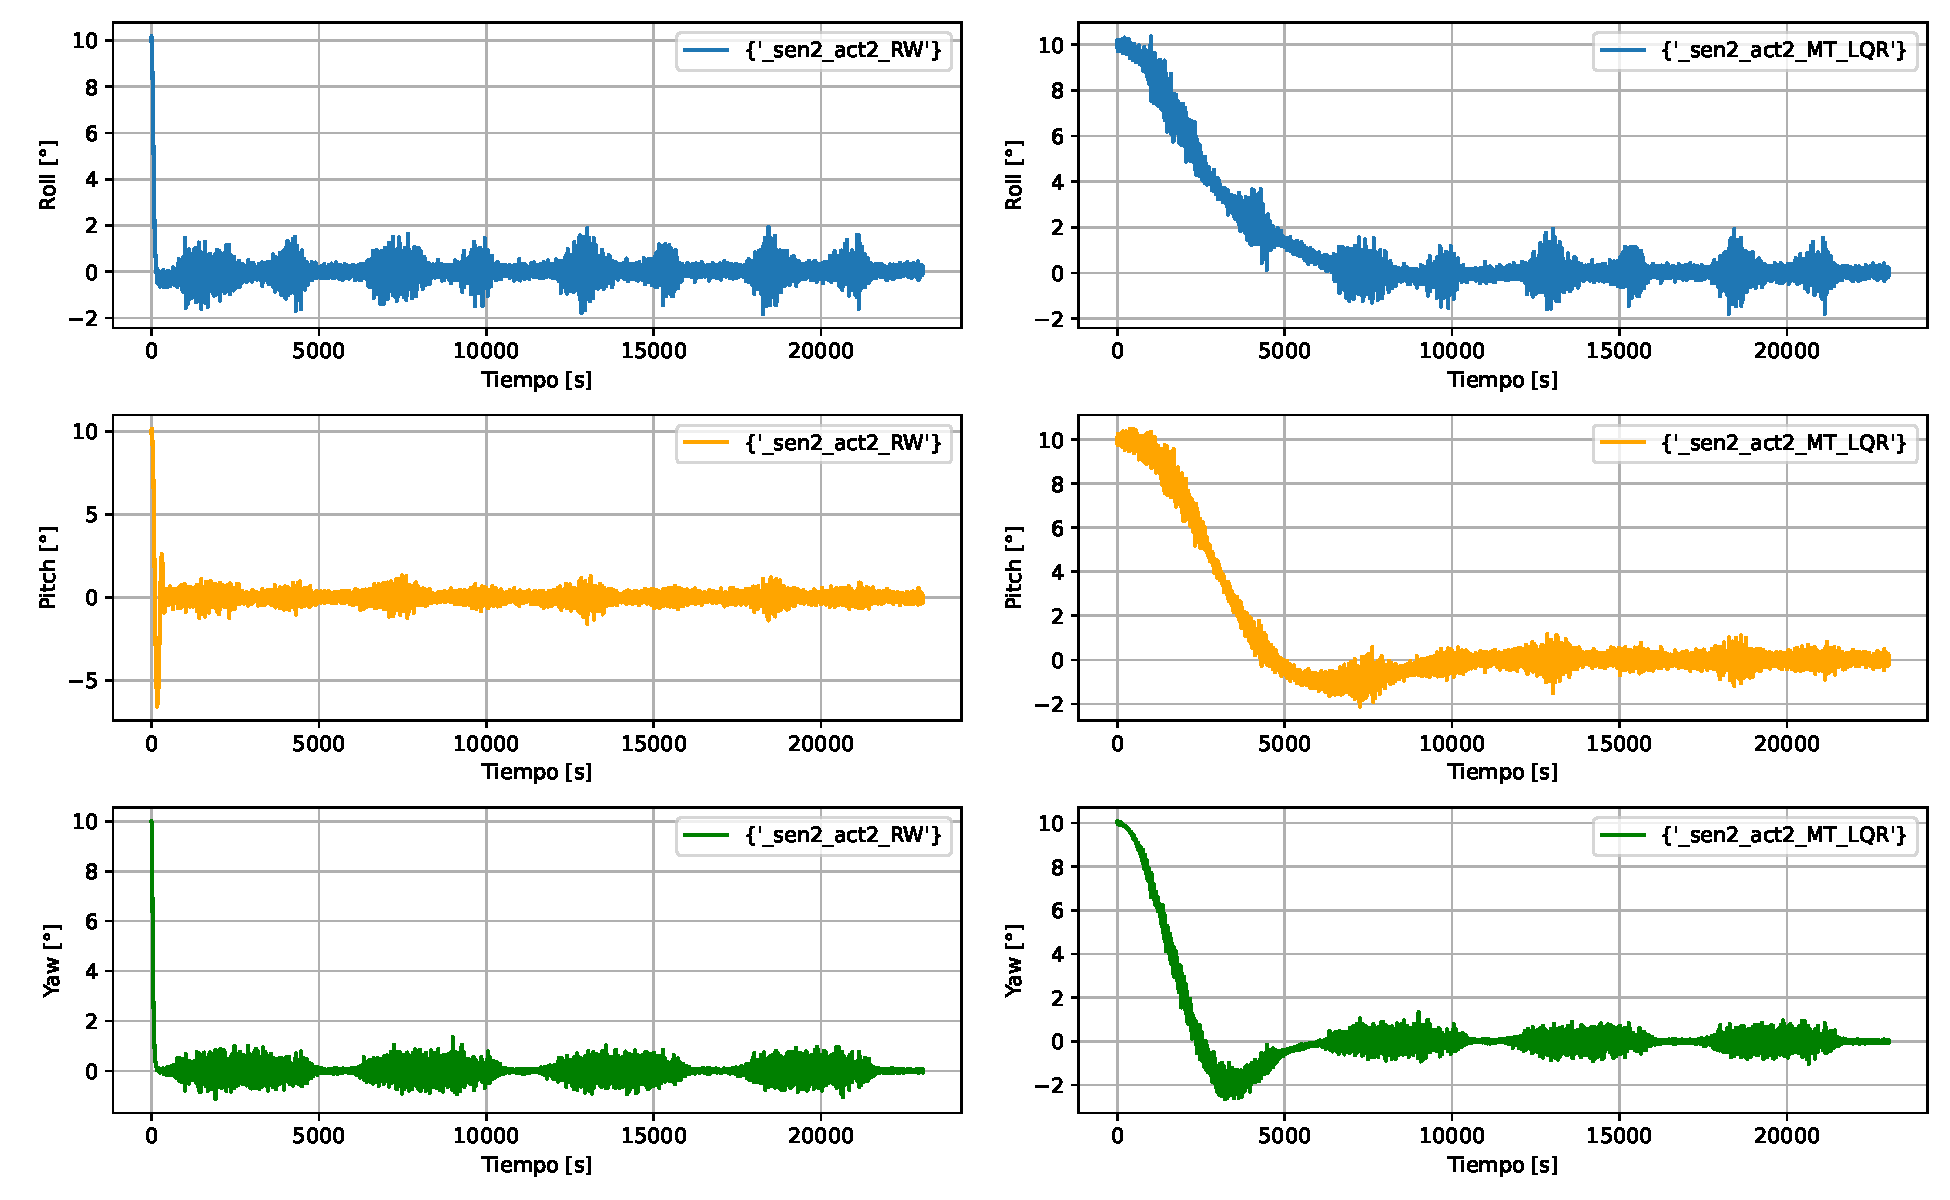
\includegraphics[width=0.97\textwidth]{MT_RW_nivel2.pdf}
	\caption{Ángulos de Euler LVLH y body para dos actuadores distintos (Elaboración propia).}
	\label{fig:MT_RW_nivel2}
\end{figure}

Además, en la Tabla~\ref{tab:RW_MT_nivel2} se observa de forma cuantitativa que las ruedas de reacción ofrecen mejores parámetros de rendimiento en términos de la norma de los MoP de apuntamiento, a cambio de un mayor consumo energético y una mayor masa en comparación con el uso de un solo actuador. Por lo tanto, según los requisitos de la misión, es fundamental que cada usuario evalúe qué opción resulta más adecuada en función de sus necesidades específicas.

\begin{table}[h!]
	\centering
	\caption{Rendimiento y costo para rueda de reaccion y magnetorquer en mismas condiciones.}
	\begin{tabular}{|c|c|c|c|c|c|}
		\hline
		\textbf{Tipo de}   & \textbf{Potencia} & \textbf{Masa [kg]} & \textbf{Accuracy [°]} & \textbf{Jitter} & \textbf{Agilidad [s]}  \\ 
		\textbf{actuador}   & \textbf{máxima [W]} & & & \textbf{[W/Hz]} &  \\
		\hline
		\textbf{Rueda de}   & 9  & 0.95  & 0.94 & 0.16 & 228   \\
		\textbf{reacción}   &  &   &  &  &    \\
		\hline
		\textbf{Magnetorquer}   & 0.8  & 0.053  & 1.71 & 0.42 & 3933   \\
		& & & & &   \\
		\hline
	\end{tabular}
	\label{tab:RW_MT_nivel2}
\end{table}


\subsubsection{Resultados de los controladores}

A continuación, se presenta un análisis comparativo entre el controlador PD y el controlador LQR aplicado al magnetorquer, con el objetivo de determinar cuál de estas opciones es más adecuada para su uso en la optimización.

En la Figura~\ref{fig:PD_LQR_nivel2}, se muestran los resultados de los ángulos de Euler llevados al equilibrio, utilizando sensores y actuadores de nivel medio (nivel 2). A la izquierda, se observa el control ejercido por el controlador PD, mientras que a la derecha, se presenta el control realizado por el controlador LQR. La Tabla~\ref{tab:PD_LQR_nivel2} resume los resultados de la norma de los MoP de apuntamiento.

La gráfica muestra que el controlador PD tarda más en estabilizar el sistema en el punto de equilibrio, utilizando los mismos componentes físicos (sensor de nivel medio y magnetorquer). Sin embargo, al estabilizarse más lentamente, se espera una mayor precisión en el apuntamiento, ya que el sistema permanece más tiempo alejado del punto de equilibrio dentro de la banda de asentamiento.

\begin{figure}[H]
	\centering    
	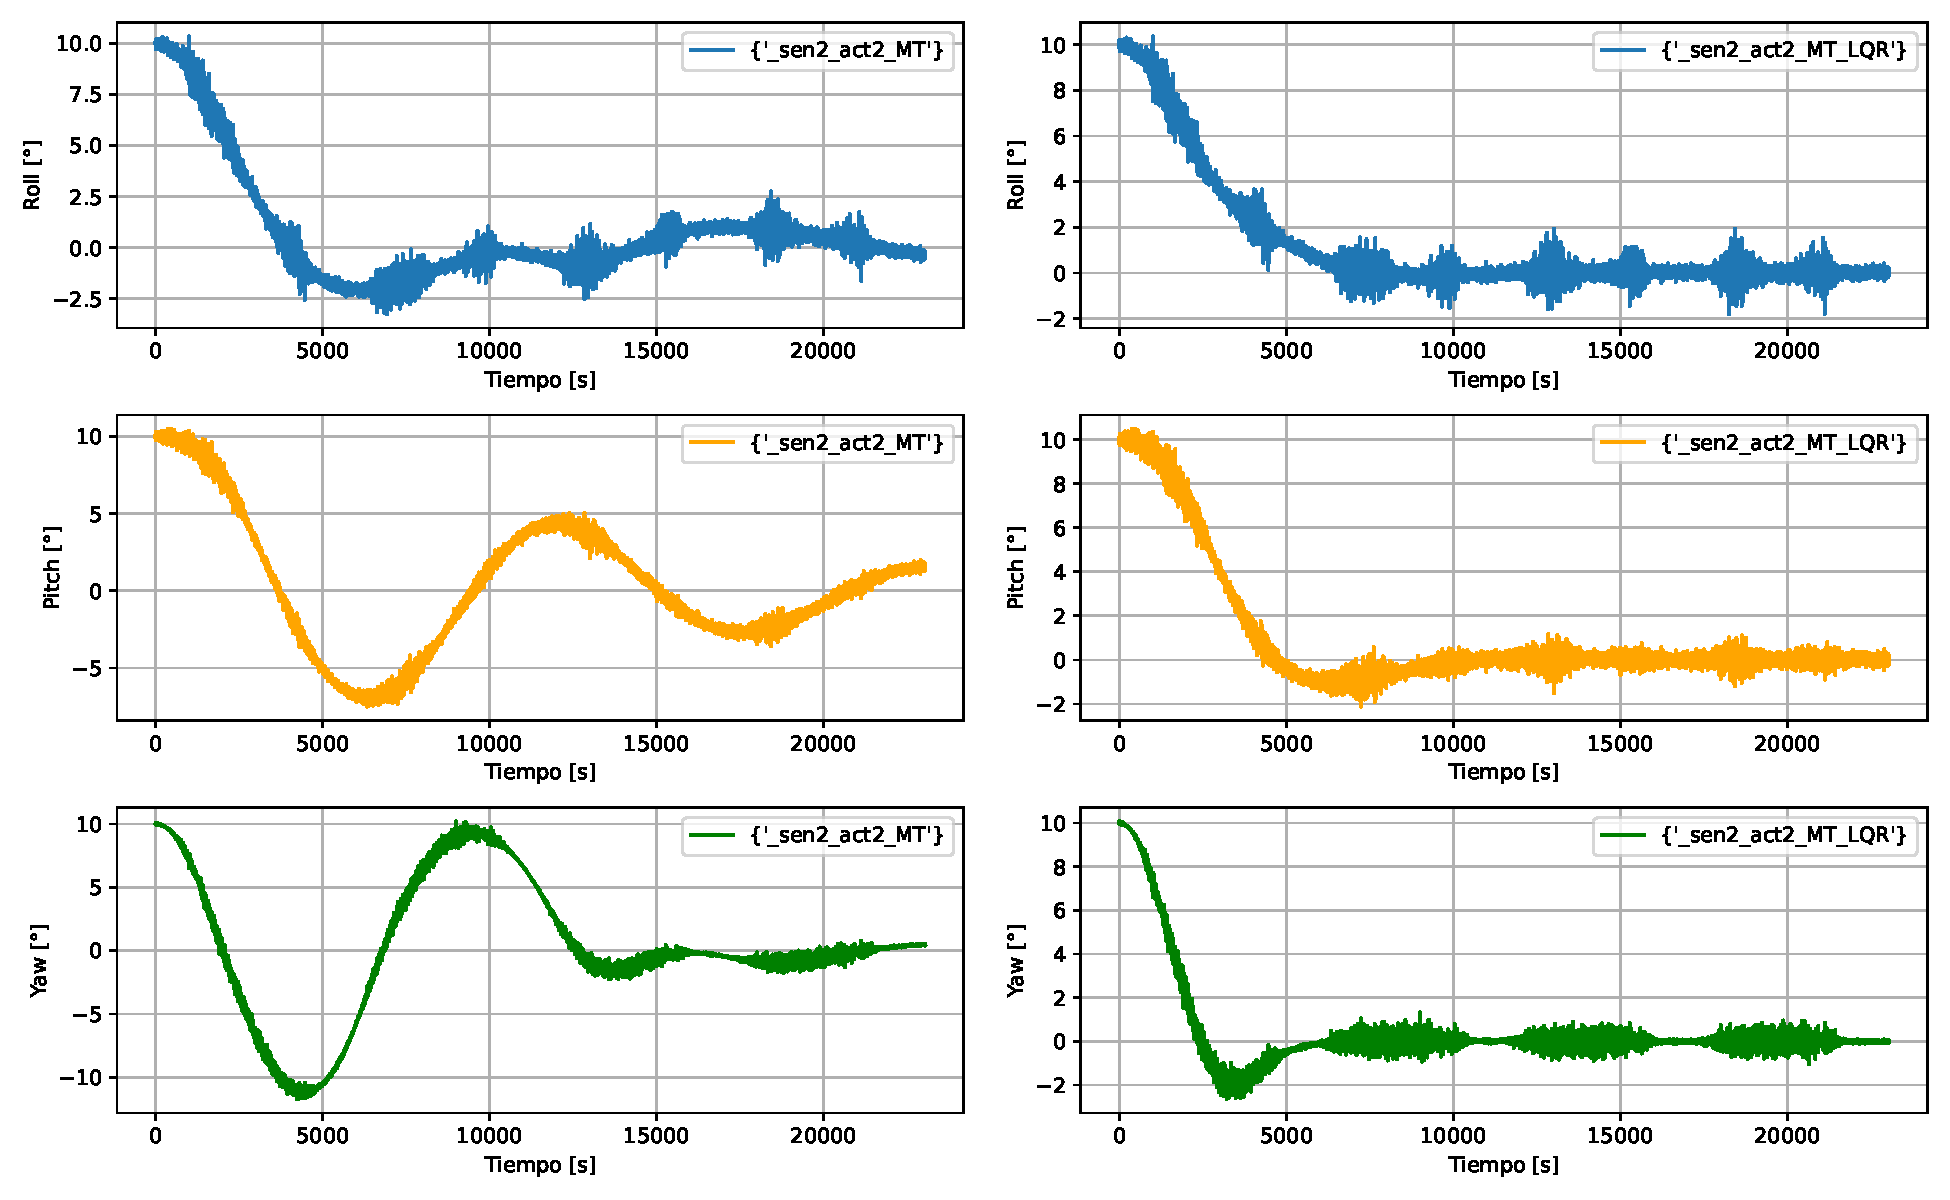
\includegraphics[width=0.97\textwidth]{PD_LQR_nivel2.pdf}
	\caption{Ángulos de Euler LVLH y body para dos controladores distintos (Elaboración propia).}
	\label{fig:PD_LQR_nivel2}
\end{figure}

Además, en la Tabla~\ref{tab:PD_LQR_nivel2} se confirma que, como se mencionó anteriormente, ambos controladores utilizan los mismos componentes, lo que implica el mismo consumo energético según la potencia máxima y la masa de los magnetorquers de nivel medio. Sin embargo, en términos de rendimiento, el controlador LQR ofrece un mejor tiempo de asentamiento y mayor precisión en el apuntamiento. Por esta razón, tanto para las ruedas de reacción como para los magnetorquers, se selecciona el controlador LQR para su implementación en la optimización dentro de la suite de simulación.

\begin{table}[h!]
	\centering
	\caption{Rendimiento y costo para controlador PD y LQR en mismas condiciones.}
	\begin{tabular}{|c|c|c|c|c|c|}
		\hline
		\textbf{Controlador}   & \textbf{Potencia} & \textbf{Masa [kg]} & \textbf{Accuracy [°]} & \textbf{Jitter} & \textbf{Agilidad [s]}  \\ 
		  & \textbf{máxima [W]} & & & \textbf{[W/Hz]} &  \\
		\hline
		\textbf{PD}   & 0.8  & 0.053  & 2.46 & 0.43 & 14040   \\
		&  &   &  &  &    \\
		\hline
		\textbf{LQR}   & 0.8  & 0.053  & 1.71 & 0.43 & 3933   \\
		& & & & &   \\
		\hline
	\end{tabular}
	\label{tab:PD_LQR_nivel2}
\end{table}

\subsubsection{Resultados niveles de sensores}

A continuación, se presenta un análisis sobre los tres niveles de sensores, utilizando actuadores de nivel 2 (medio), con el fin de evaluar cómo la estimación de la actitud del satélite, basada en los diferentes niveles de sensores, afecta los MoP de apuntamiento y su costo asociado.

En la Figura~\ref{fig:MT_LQR_sensores}, se muestran tres columnas de gráficas que representan el control de los ángulos de Euler hacia el equilibrio. En la primera columna, a la izquierda, se observa la simulación de actitud basada en los ángulos de Roll, Pitch y Yaw utilizando sensores de nivel 1 (bajo). La segunda columna muestra el caso con sensores de nivel 2 (medio), mientras que la tercera columna, a la derecha, corresponde a sensores de nivel 3 (alto). La Tabla~\ref{tab:MT_LQR_sensores} resume los resultados de los MoP de apuntamiento junto con los costos asociados a los distintos niveles de magnetómetro y sensor solar.

En la gráfica, se puede observar que, con sensores de nivel bajo, existe mayor ruido y dispersión en los ángulos de Euler una vez estabilizados en el equilibrio. Este comportamiento mejora conforme se incrementa el nivel de los sensores, mostrando una menor dispersión en los ángulos de Euler, lo que resulta en una mejora de la precisión de apuntamiento y una reducción del jitter.

\begin{figure}[H]
	\centering    
	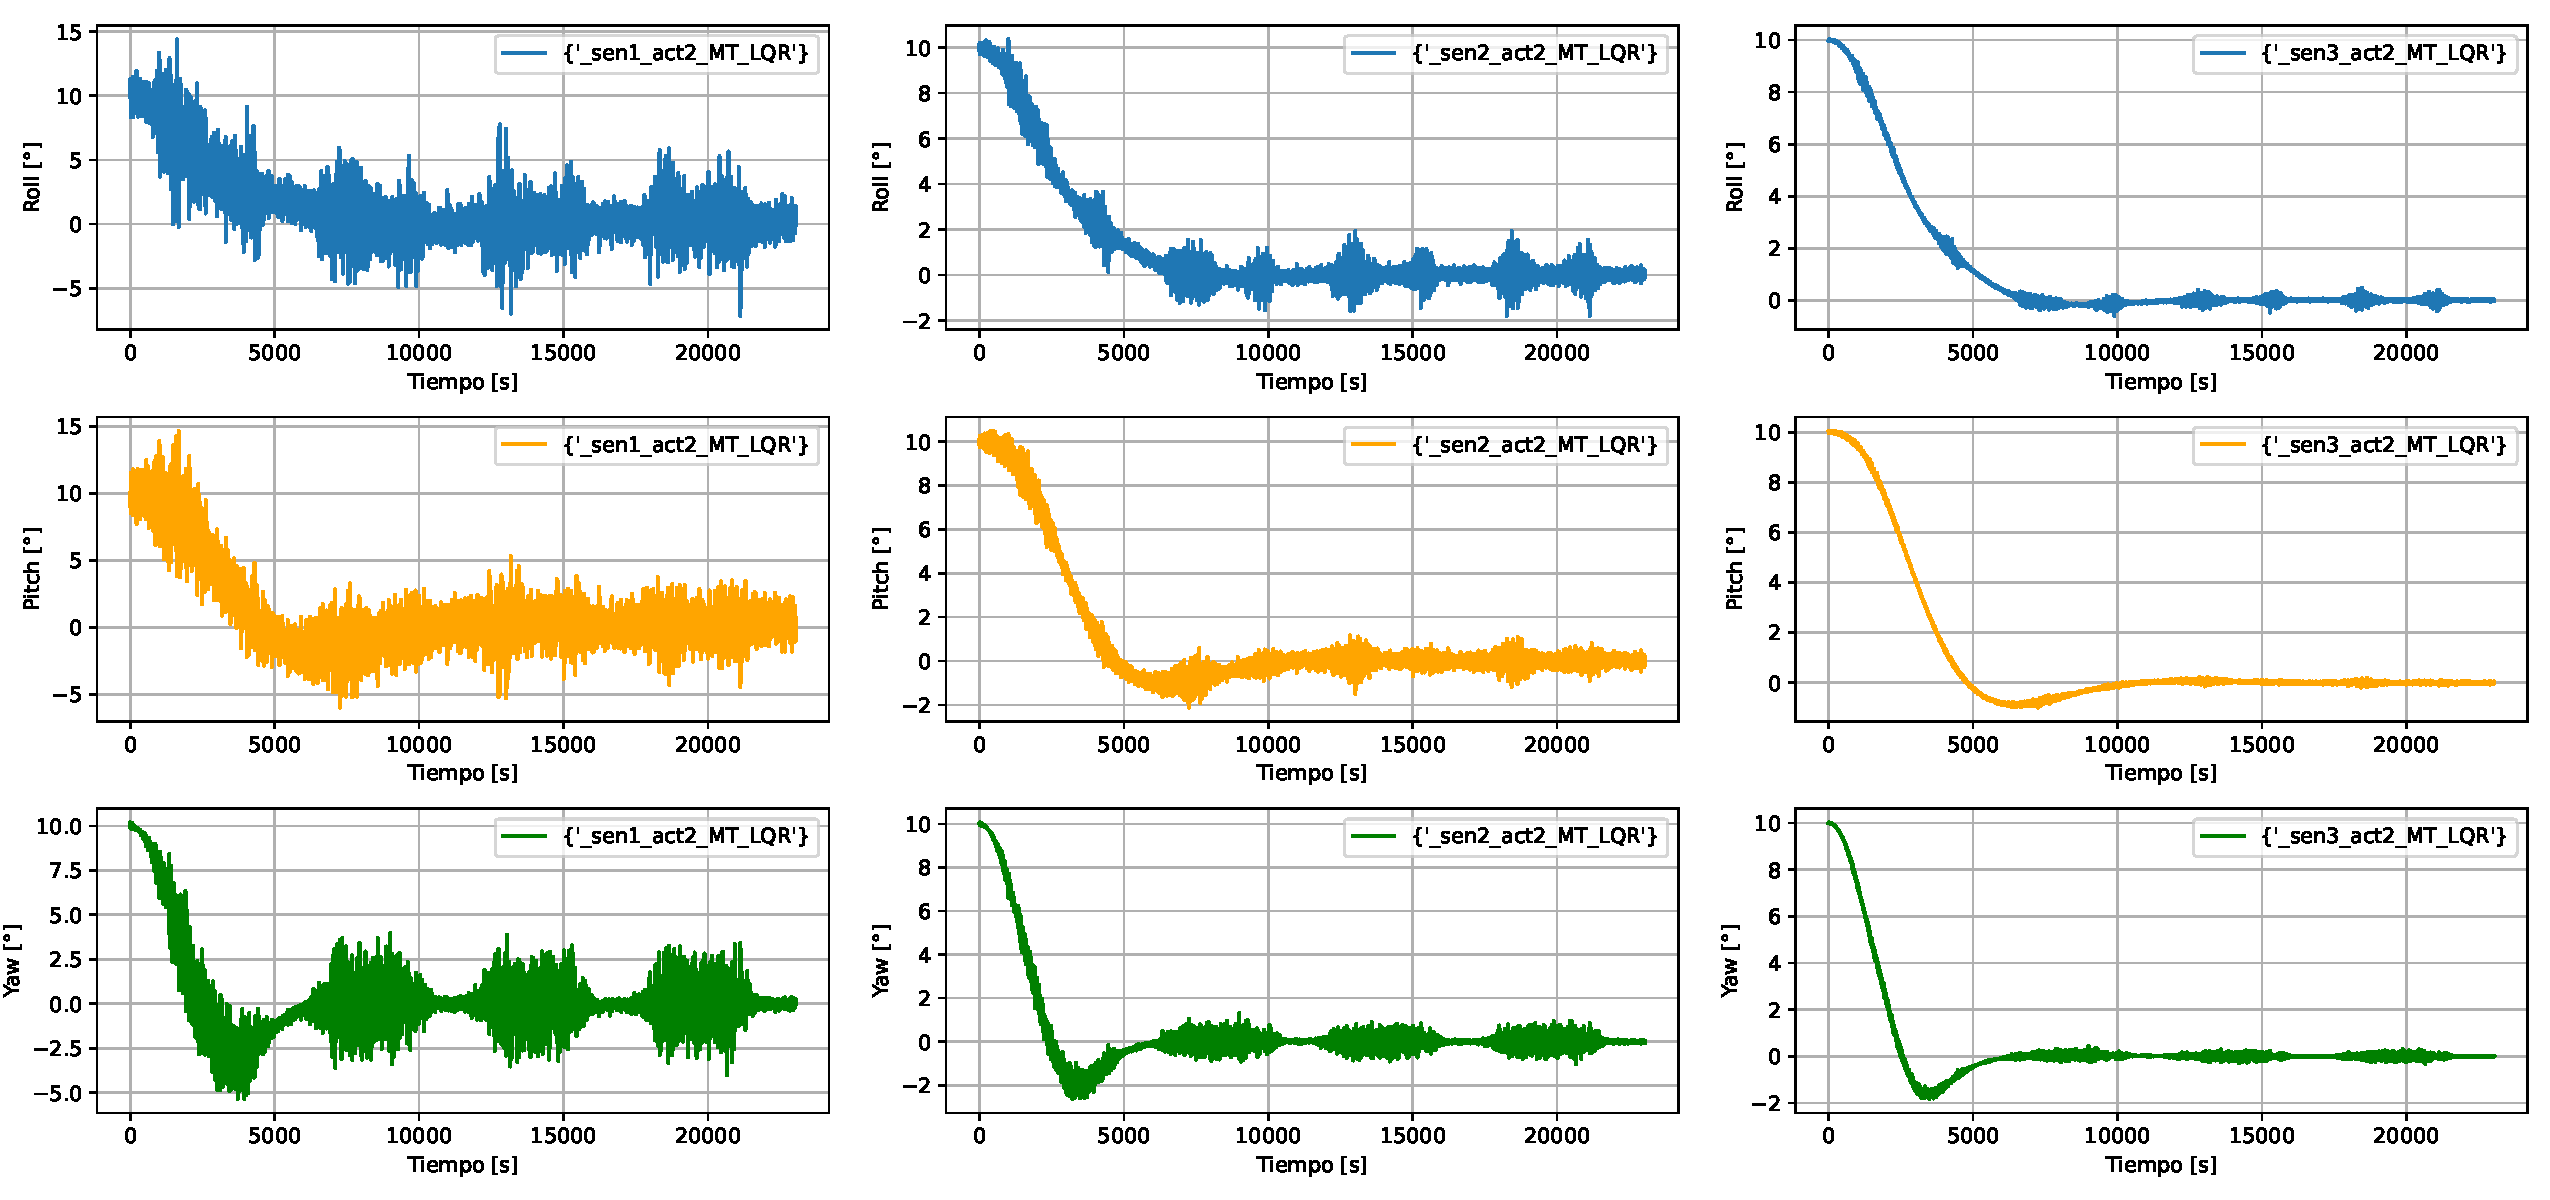
\includegraphics[width=0.97\textwidth]{MT_LQR_sensores.pdf}
	\caption{Ángulos de Euler LVLH y body para niveles de sensor distintos con magnetorquer (Elaboración propia).}
	\label{fig:MT_LQR_sensores}
\end{figure}

Además, en la Tabla~\ref{tab:MT_LQR_sensores} se confirma que la mejora en el nivel de los sensores contribuye significativamente a un mejor rendimiento en la precisión de apuntamiento y en la reducción del jitter. Sin embargo, una observación importante es que, aunque el paso de sensores de nivel medio a nivel alto mejoró la exactitud de apuntamiento, no tuvo un impacto notable en la reducción del jitter. En cuanto a la agilidad, el efecto de los sensores en la mejora del tiempo de asentamiento fue mínimo, lo que indica que este componente físico no está directamente relacionado con dicho MoP de apuntamiento.

\begin{table}[h!]
	\centering
	\caption{Rendimiento y costo para niveles de sensor con nivel 2 de magnetorquer y LQR.}
	\begin{tabular}{|c|c|c|c|c|c|}
		\hline
		\textbf{Nivel de}   & \textbf{Potencia} & \textbf{Masa [kg]} & \textbf{Accuracy [°]} & \textbf{Jitter} & \textbf{Agilidad [s]}  \\ 
		\textbf{sensor}  & \textbf{máxima [W]} & & & \textbf{[W/Hz]} &  \\
		\hline
		\textbf{Nivel 1}   & 0.15  & 0.067  & 3.72 & 2.92 & 4081   \\
		&  &   &  &  &    \\
		\hline
		\textbf{Nivel 2}   & 0.3  & 0.181  & 1.71 & 0.43 & 3933   \\
		& & & & &   \\
		\hline
		\textbf{Nivel 3}   & 0.75  & 0.530  & 1.5 & 0.43 & 3957   \\
		& & & & &   \\
		\hline		
	\end{tabular}
	\label{tab:MT_LQR_sensores}
\end{table}

En la Figura~\ref{fig:RW_LQR_sensores} se presenta el mismo análisis de sensores, pero en este caso utilizando las ruedas de reacción como actuador de nivel 2. También se muestran los resultados de los MoP de apuntamiento y el costo asociado a los sensores en la Tabla~\ref{tab:RW_LQR_sensores}.

En la gráfica, al igual que con los magnetorquers, se puede observar un mayor ruido y dispersión en los datos de los ángulos de Euler cuando se utilizan sensores de nivel bajo. Esta dispersión disminuye a medida que se incrementa la calidad de los magnetómetros y los sensores solares, evidenciándose una menor variabilidad en los datos una vez que se alcanza el equilibrio.

\begin{figure}[H]
	\centering    
	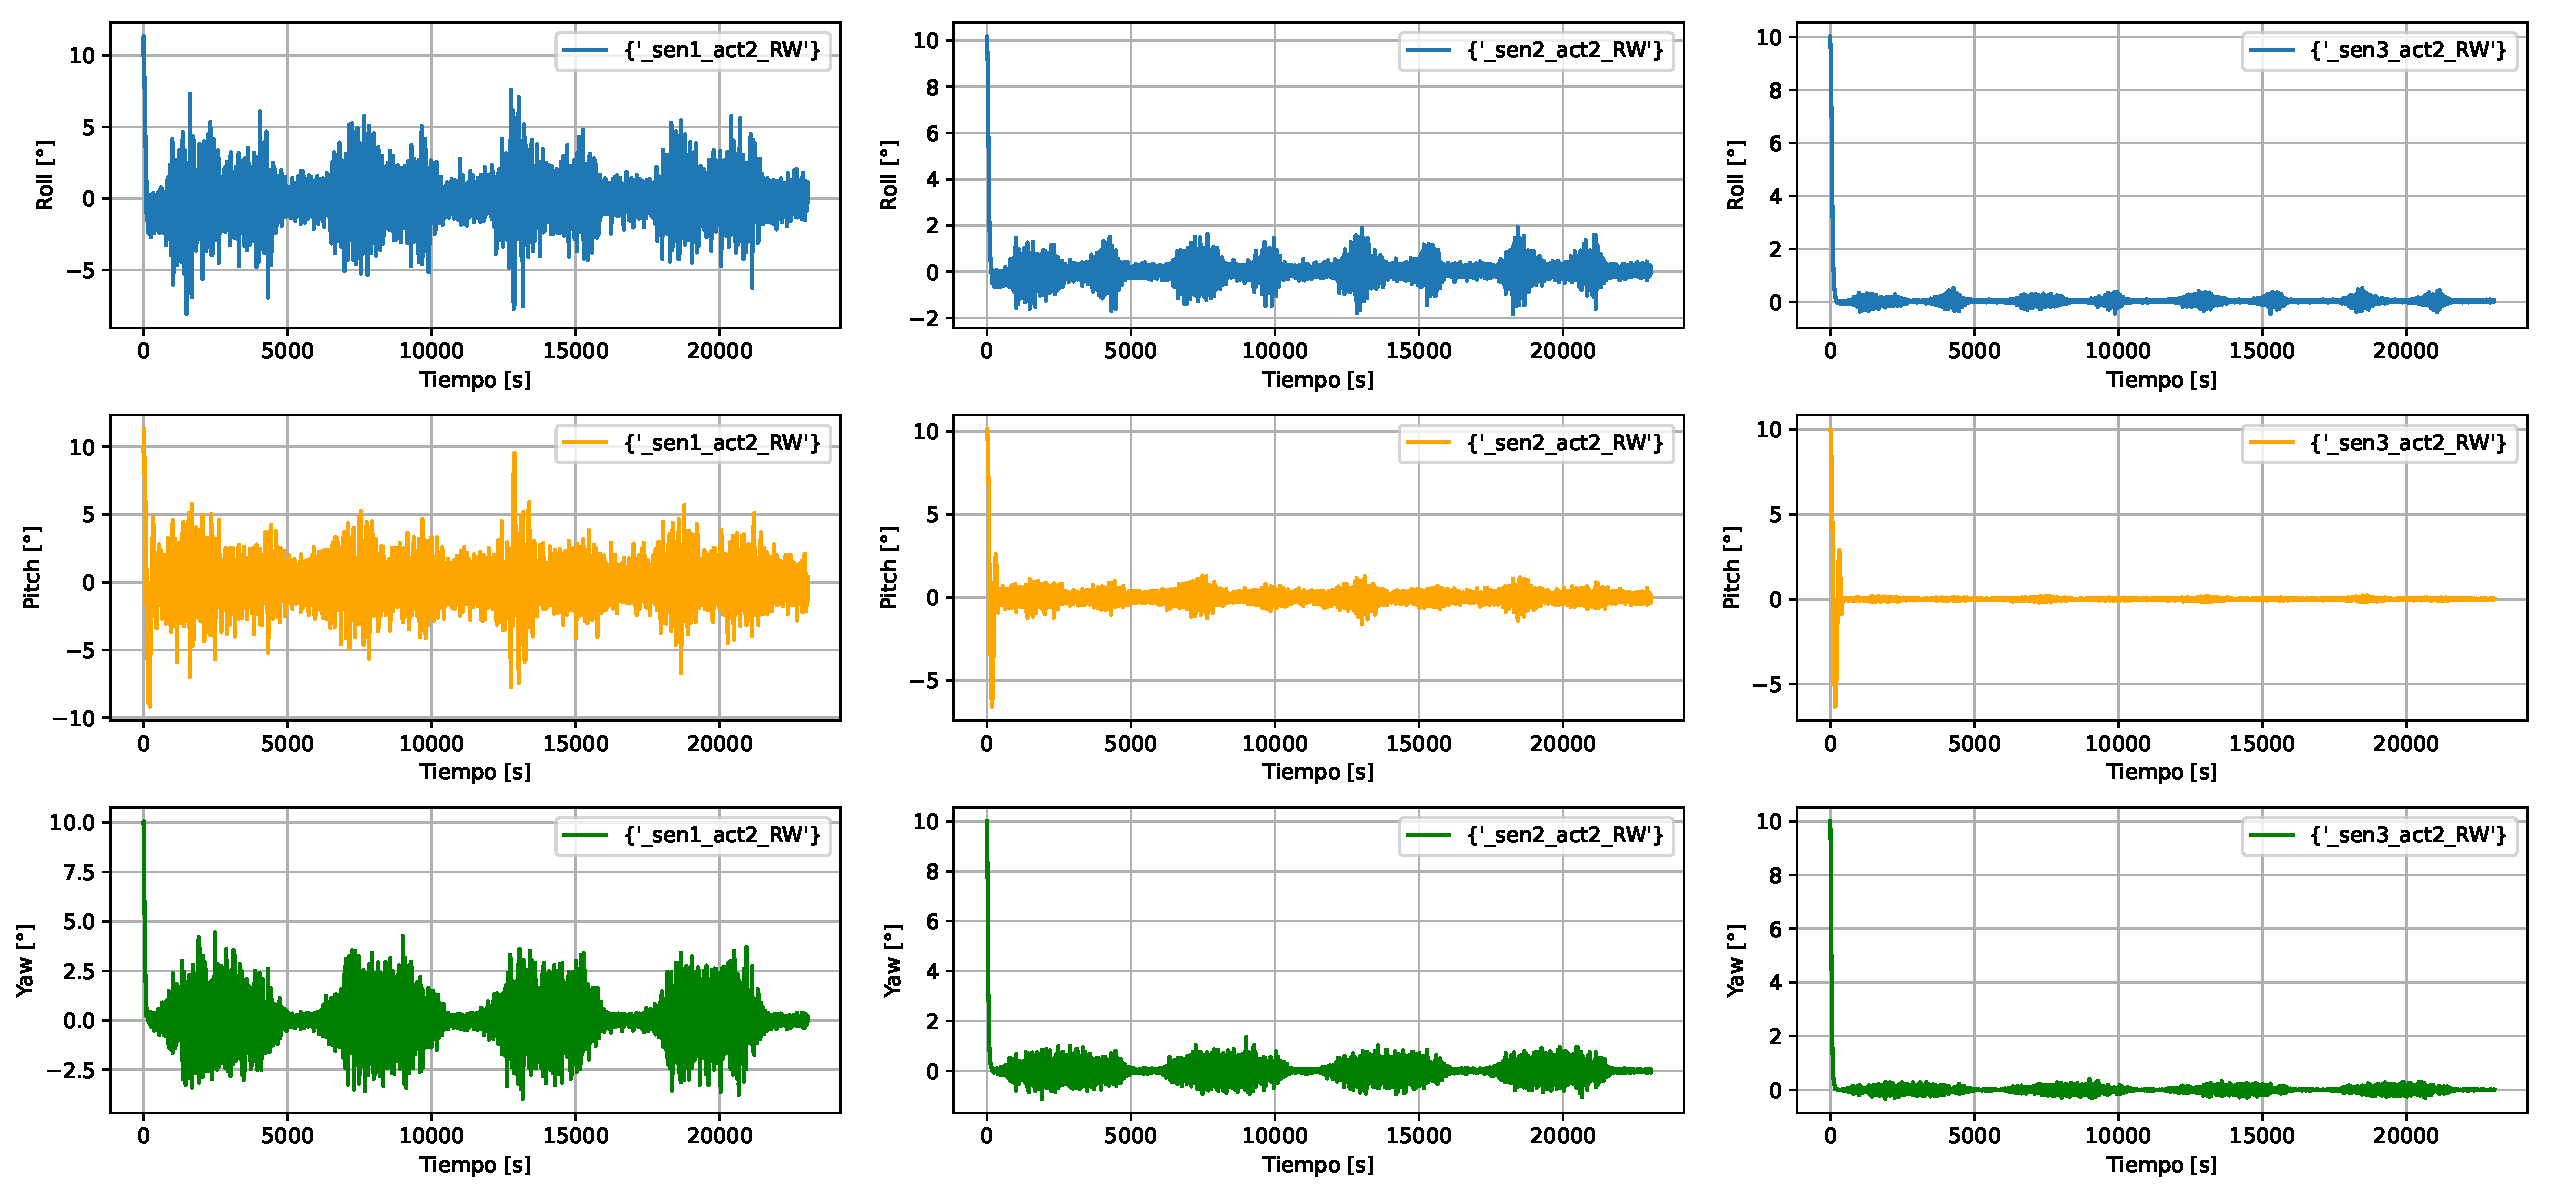
\includegraphics[width=0.97\textwidth]{RW_LQR_sensores.pdf}
	\caption{Ángulos de Euler LVLH y body para niveles de sensor distintos con rueda de reacción (Elaboración propia).}
	\label{fig:RW_LQR_sensores}
\end{figure}

En la Tabla~\ref{tab:RW_LQR_sensores}, se confirma lo mencionado anteriormente: se observa una mejora notable en la exactitud de apuntamiento y en el jitter al pasar de sensores de nivel bajo a medio, aunque esto conlleva un incremento significativo en el consumo de potencia y energía debido al uso de sensores de mayor calidad.

Un aspecto particular del caso de las ruedas de reacción es que, a diferencia de lo observado con los magnetorquers, en cada nivel se manifiesta una mejora en el jitter. En el caso de los magnetorquers, no se notó esta mejora al pasar del nivel 2 al nivel 3, donde los valores se mantuvieron constantes. Además, no se observa una mejora en la agilidad al incrementar el nivel de los sensores, como se evidencia en la tabla, donde los tiempos de asentamiento permanecen sin variaciones a pesar de la mejora en el componente físico.

\begin{table}[h!]
	\centering
	\caption{Rendimiento y costo para niveles de sensor con nivel 2 de rueda de reacción y LQR.}
	\begin{tabular}{|c|c|c|c|c|c|}
		\hline
		\textbf{Nivel de}   & \textbf{Potencia} & \textbf{Masa [kg]} & \textbf{Accuracy [°]} & \textbf{Jitter} & \textbf{Agilidad [s]}  \\ 
		\textbf{sensor}  & \textbf{máxima [W]} & & & \textbf{[W/Hz]} &  \\
		\hline
		\textbf{Nivel 1}   & 0.15  & 0.067  & 3.76 & 3.28 & 230  \\
		&  &   &  &  &    \\
		\hline
		\textbf{Nivel 2}   & 0.3  & 0.181  & 0.93 & 0.16 & 228   \\
		& & & & &   \\
		\hline
		\textbf{Nivel 3}   & 0.75  & 0.530  & 0.52 & 0.02 & 229   \\
		& & & & &   \\
		\hline		
	\end{tabular}
	\label{tab:RW_LQR_sensores}
\end{table}

\subsubsection{Resultados niveles de actuadores}

A continuación, se presentan análisis sobre los tres niveles de actuadores, utilizando sensores de nivel 2 (medio), para evaluar cómo la estimación de la actitud del satélite, en función de los diferentes niveles de actuadores, afecta los MoP de apuntamiento y su costo asociado.

En la Figura~\ref{fig:MT_LQR_actuadores}, se muestran tres columnas de gráficas que representan el control de los ángulos de Euler hacia el equilibrio. En la primera columna, a la izquierda, se presenta la simulación de actitud basada en los ángulos de Roll, Pitch y Yaw, utilizando magnetorquers de nivel 1. Las segunda y tercera columnas muestran el mismo análisis para los niveles 2 y 3, respectivamente. La Tabla~\ref{tab:MT_LQR_actuadores} resume los resultados de los MoP de apuntamiento y el costo asociado a los magnetorquers.

En la gráfica, se puede observar que, con actuadores de nivel bajo, el control es más suave, ya que el sistema tarda más tiempo en asentarse en el equilibrio. Sin embargo, esta situación mejora al utilizar magnetorquers de mayor calidad, como se evidencia en las otras dos columnas. Este comportamiento de mejora en el control hacia el equilibrio se aprecia con mayor claridad en la gráfica correspondiente al Yaw (verde).

\begin{figure}[H]
	\centering    
	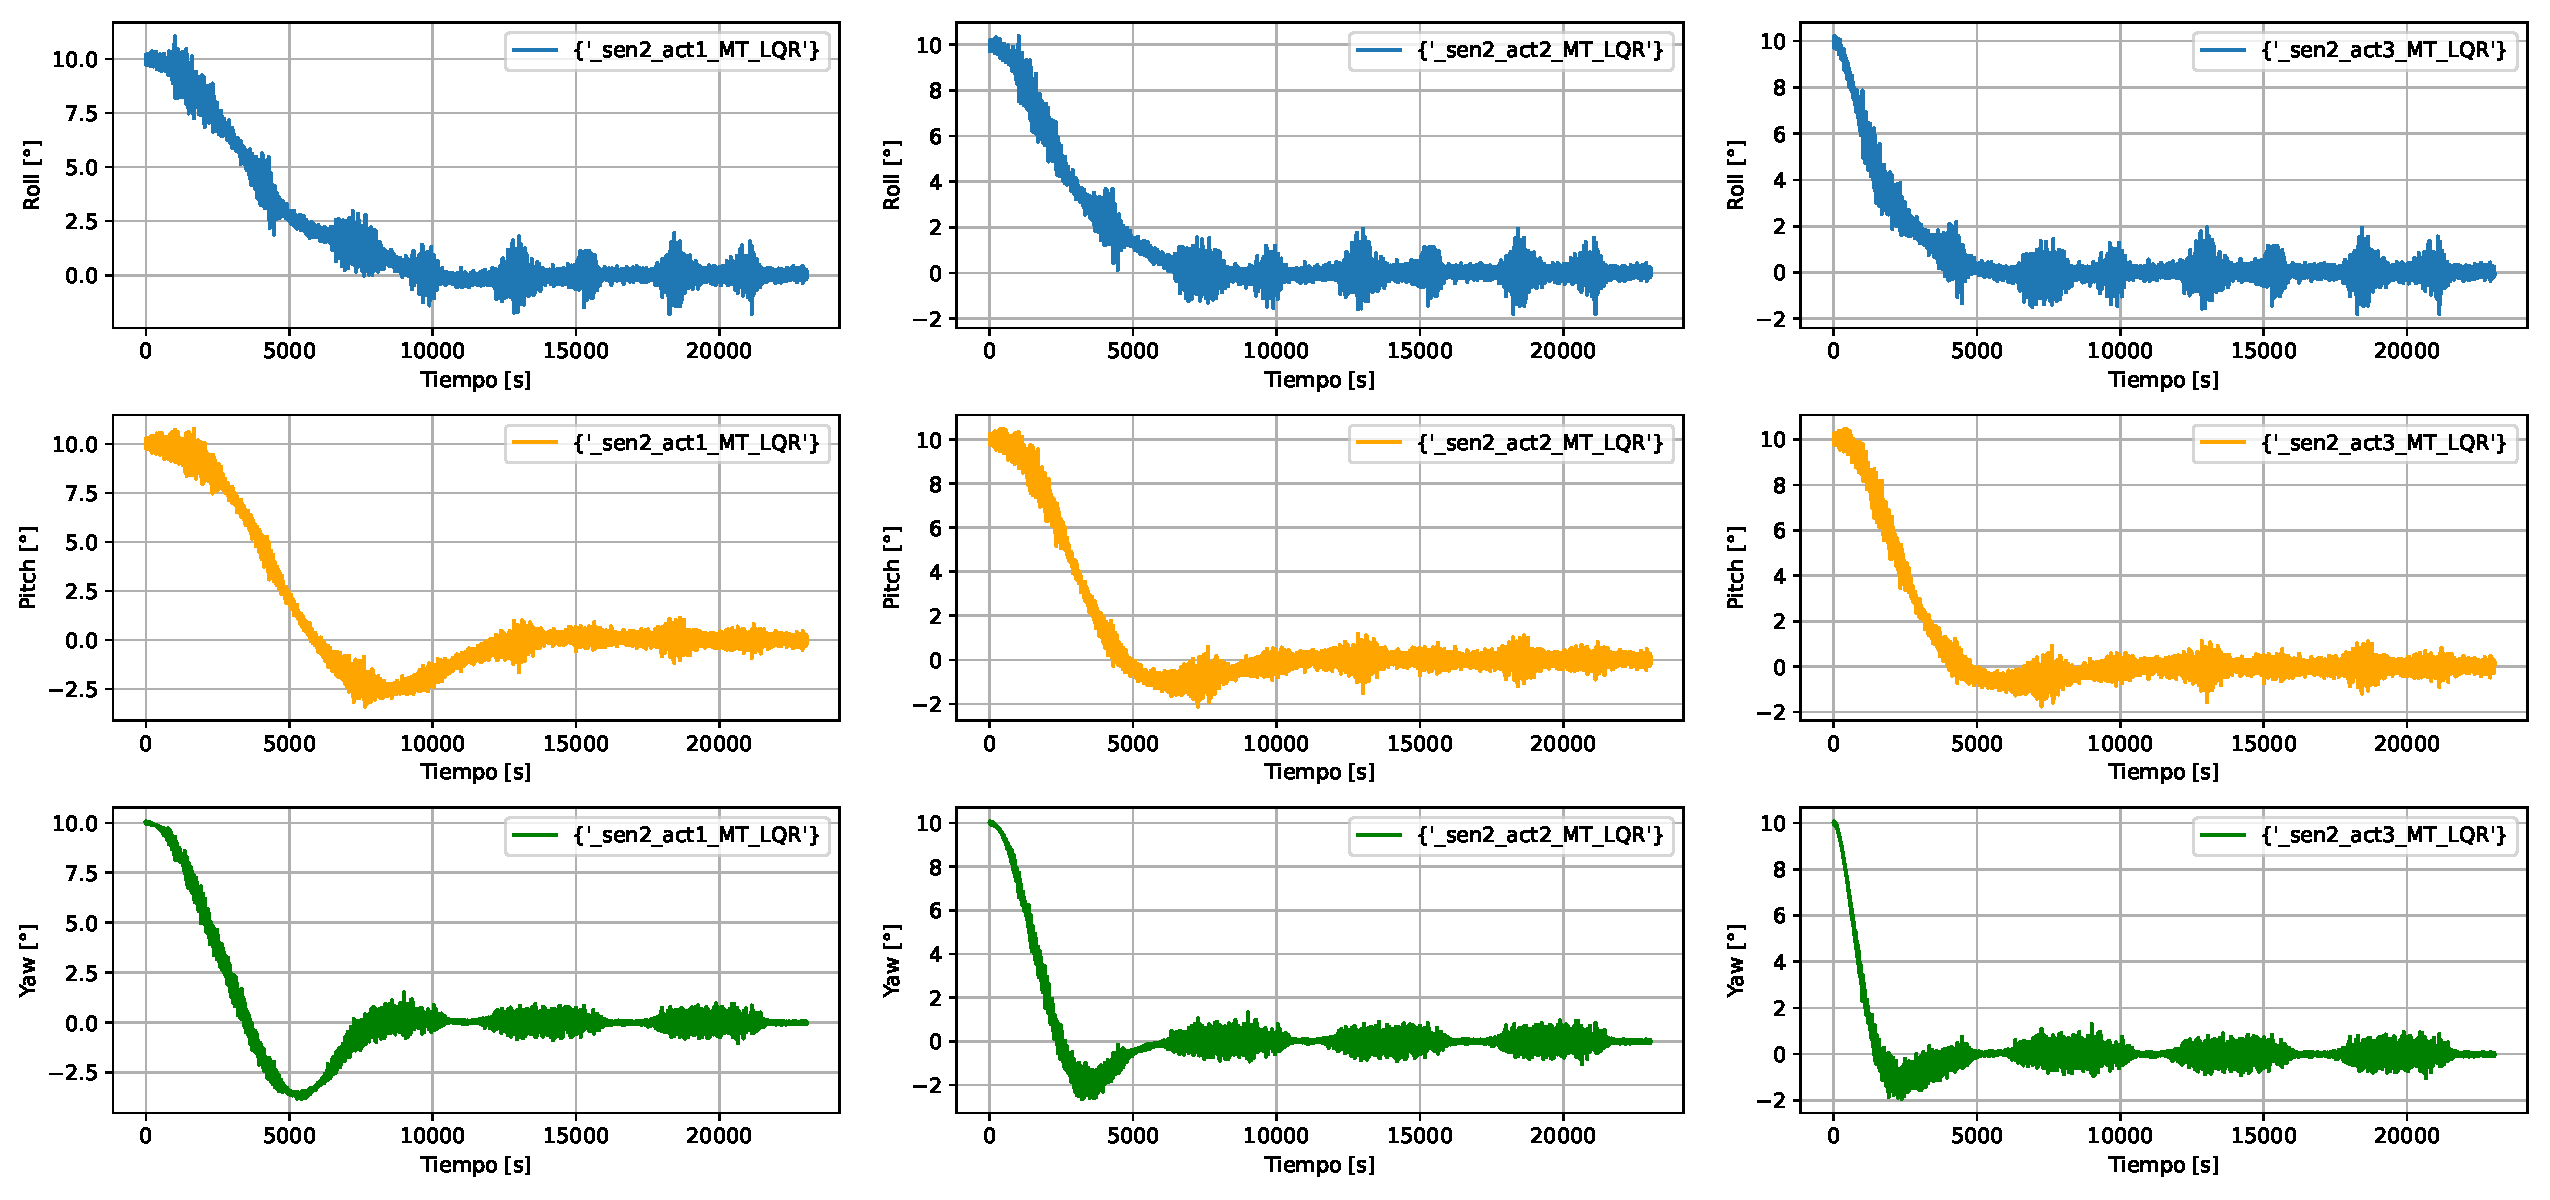
\includegraphics[width=0.97\textwidth]{MT_LQR_actuadores.pdf}
	\caption{Ángulos de Euler LVLH y body para niveles de magnetorquer distintos con sensores nivel 2 (Elaboración propia).}
	\label{fig:MT_LQR_actuadores}
\end{figure}

En la Tabla~\ref{tab:MT_LQR_actuadores}, se observa que, a medida que se incrementa el nivel de los magnetorquers, la norma de la exactitud de apuntamiento mejora del nivel 1 al nivel 2, pero se deteriora al alcanzar el nivel 3. También se nota una disminución en el tiempo de asentamiento, un aspecto que se representa de manera más clara en la gráfica.

Sin embargo, al aumentar el nivel del magnetorquer, se evidencia un incremento en el ruido, reflejado por el jitter. Este fenómeno se debe a que un mayor torque debido al campo magnético, genera vibraciones mecánicas que afectan la densidad espectral de potencia. A partir de los resultados, se puede concluir que existe una tendencia clara que indica que los magnetorquers están directamente relacionados con la mejora del tiempo de asentamiento. Sin embargo, es importante destacar que, dependiendo del caso, este aumento en el nivel del actuador puede no necesariamente traducirse en una mejora de la exactitud de apuntamiento, lo que sugiere que no hay una relación directa entre ambas variables en todas las situaciones.

\begin{table}[h!]
	\centering
	\caption{Rendimiento y costo para niveles de magnetorquer con nivel 2 de sensor y LQR.}
	\begin{tabular}{|c|c|c|c|c|c|}
		\hline
		\textbf{Nivel de}   & \textbf{Potencia} & \textbf{Masa [kg]} & \textbf{Accuracy [°]} & \textbf{Jitter} & \textbf{Agilidad [s]}  \\ 
		\textbf{actuador}  & \textbf{máxima [W]} & & & \textbf{[W/Hz]} &  \\
		\hline
		\textbf{Nivel 1}   & 0.275  &  0.03  & 3.09 &  0.41 & 5821   \\
		&  &   &  &  &    \\
		\hline
		\textbf{Nivel 2}   & 0.8  & 0.053  & 1.71 & 0.43 & 3933   \\
		& & & & &   \\
		\hline
		\textbf{Nivel 3}   & 1.11  & 0.43  & 1.83 & 0.49 & 2692   \\
		& & & & &   \\
		\hline		
	\end{tabular}
	\label{tab:MT_LQR_actuadores}
\end{table}

En la Figura~\ref{fig:RW_LQR_actuadores}, se presenta el mismo análisis aplicado a las ruedas de reacción, utilizando nuevamente sensores de nivel 2. Además, los resultados de los MoP de apuntamiento y el costo asociado a los actuadores se detallan en la Tabla~\ref{tab:RW_LQR_actuadores}.

En la gráfica, se observa un comportamiento similar al observado en el caso de los magnetorquers. A medida que se mejora el nivel del actuador, se evidencia una mejora en el control hacia el tiempo de asentamiento en los ángulos de Euler. Las gráficas muestran leves diferencias en la dispersión de datos y el ruido, lo que sugiere que, a simple vista, estos factores no afectan significativamente los demás MoP de apuntamiento analizados.

\begin{figure}[H]
	\centering    
	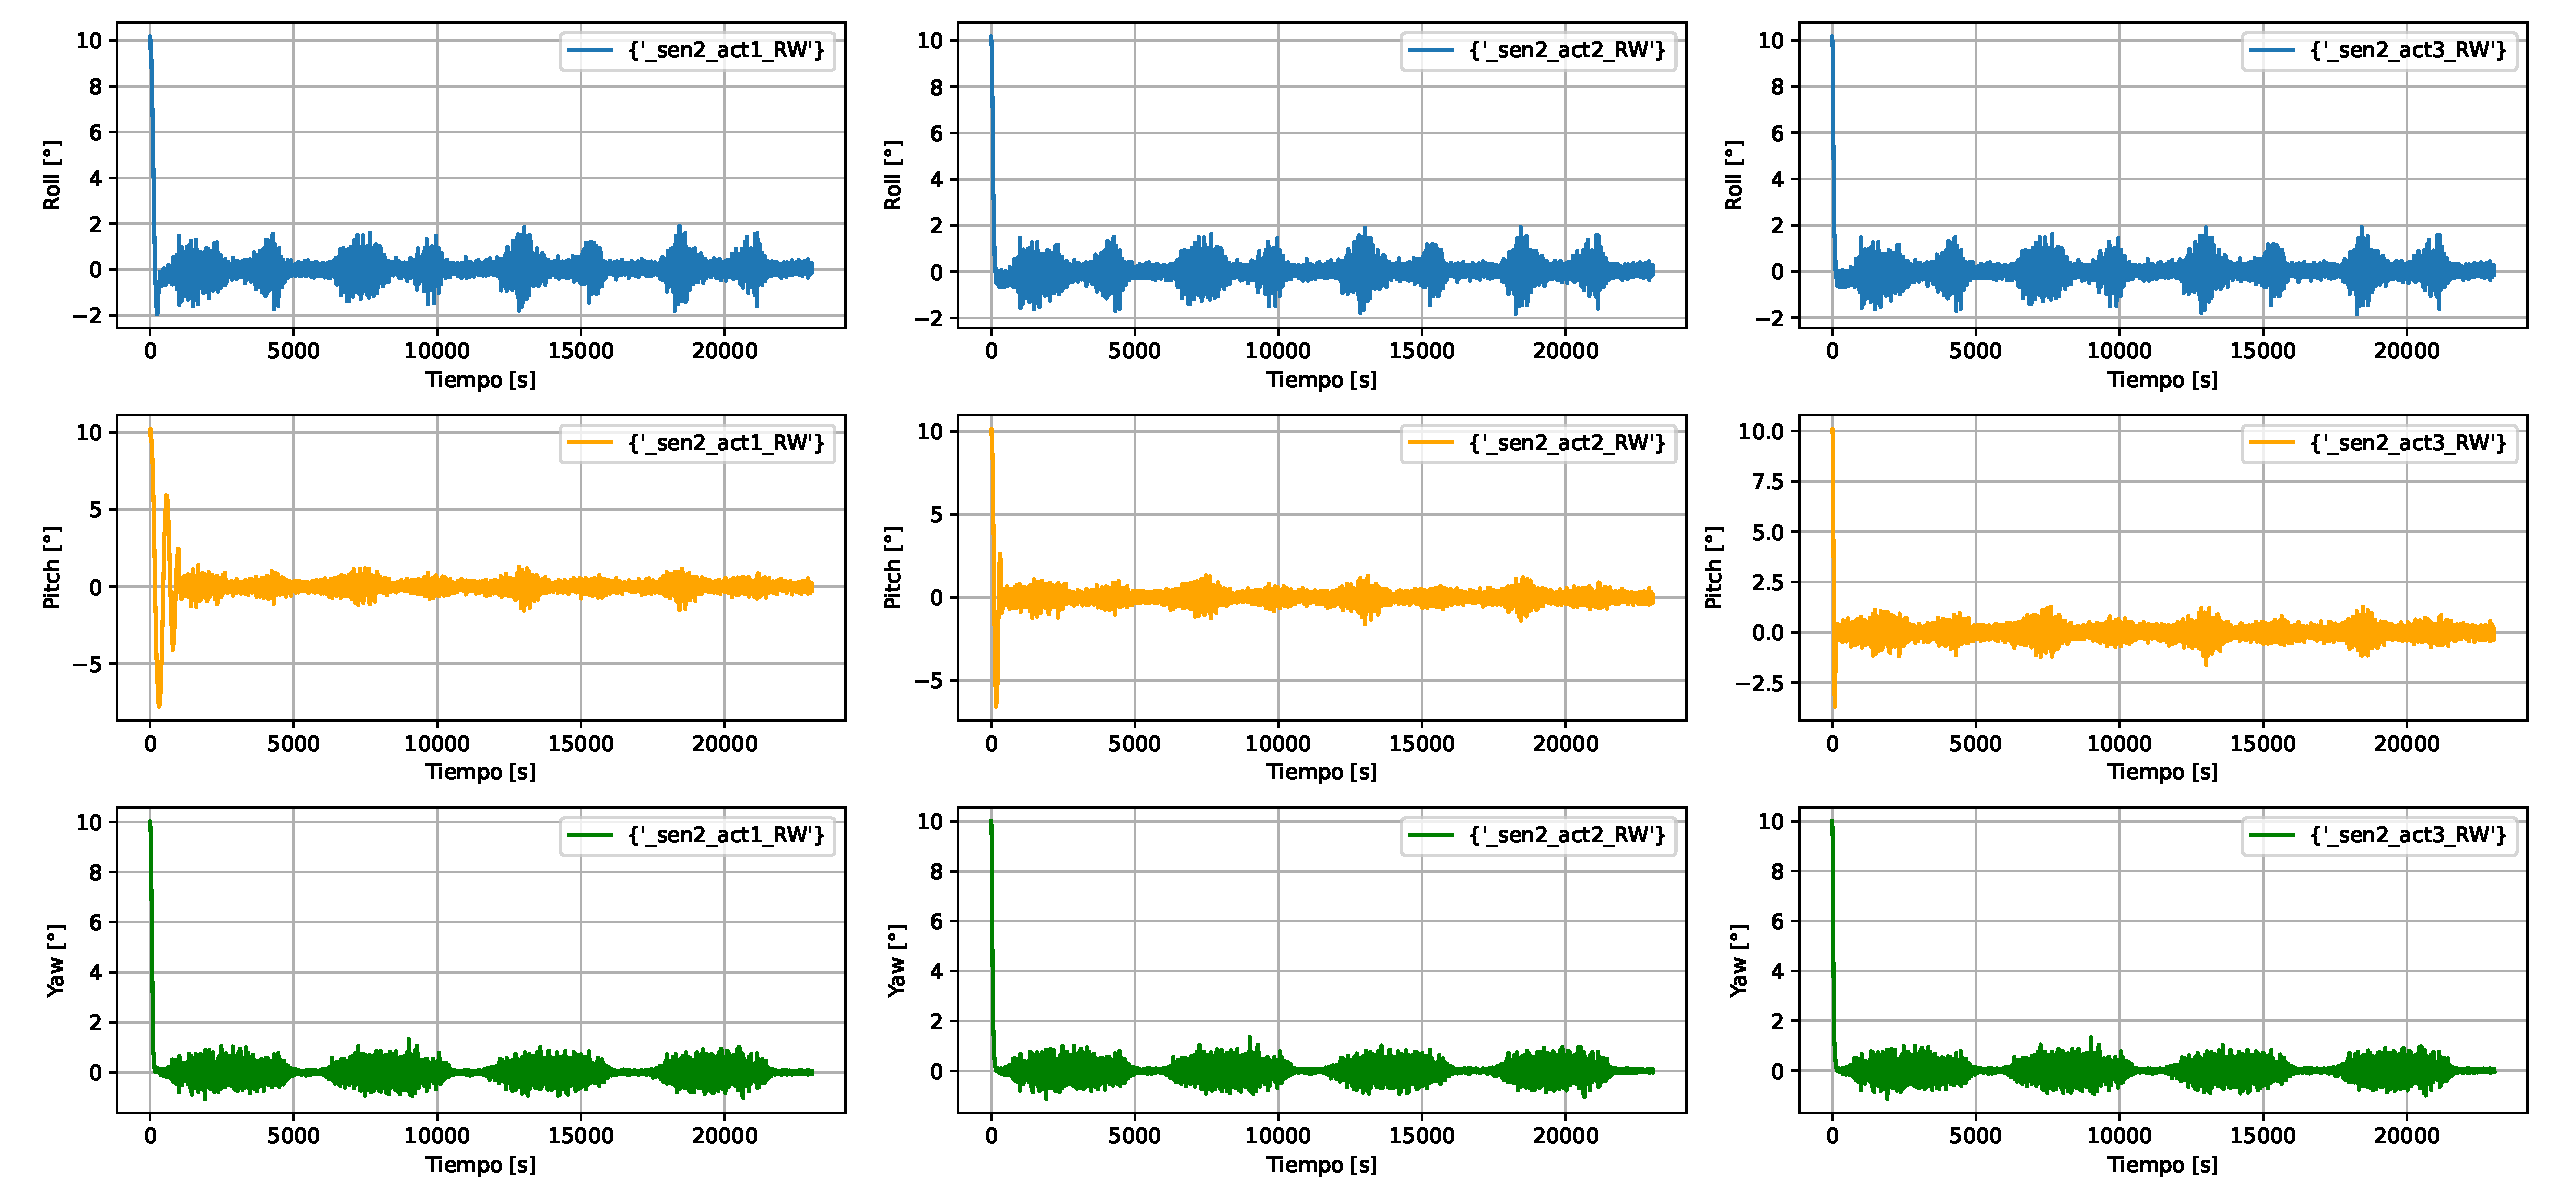
\includegraphics[width=0.97\textwidth]{RW_LQR_actuadores.pdf}
	\caption{Ángulos de Euler LVLH y body para niveles de rueda de reacción distintos con sensores nivel 2 (Elaboración propia).}
	\label{fig:RW_LQR_actuadores}
\end{figure}


En la Tabla~\ref{tab:RW_LQR_actuadores}, se puede observar que una mejora en el nivel de las ruedas de reacción implica un costo significativamente mayor, especialmente en comparación con los magnetorquers. Este aumento de costo se traduce en una mejora en el tiempo de asentamiento, así como en una mejora del jitter y, en menor medida, en la exactitud de apuntamiento. Sin embargo, es importante señalar que, a pesar de la mejora en el nivel de las ruedas de reacción, el impacto en la exactitud de apuntamiento no es significativo, lo cual se refleja también en las gráficas.

\begin{table}[h!]
	\centering
	\caption{Rendimiento y costo para niveles de rueda de reacción con nivel 2 de sensor y LQR.}
	\begin{tabular}{|c|c|c|c|c|c|}
		\hline
		\textbf{Nivel de}   & \textbf{Potencia} & \textbf{Masa [kg]} & \textbf{Accuracy [°]} & \textbf{Jitter} & \textbf{Agilidad [s]}  \\ 
		\textbf{sensor}  & \textbf{máxima [W]} & & & \textbf{[W/Hz]} &  \\
		\hline
		\textbf{Nivel 1}   & 6  & 0.75  & 1.18 & 0.36 & 628  \\
		&  &   &  &  &    \\
		\hline
		\textbf{Nivel 2}   & 9  & 0.95  & 0.93 & 0.16 & 228   \\
		& & & & &   \\
		\hline
		\textbf{Nivel 3}   & 10  & 3.2  & 0.95 & 0.15 & 63   \\
		& & & & &   \\
		\hline		
	\end{tabular}
	\label{tab:RW_LQR_actuadores}
\end{table}

\subsection{Resumen sobre análisis realizados}

Al analizar los resultados obtenidos con la suite de simulación, se pueden establecer las siguientes conclusiones:

\begin{itemize}
	\item \textbf{Rueda de reacción vs Magnetorquer:} A partir de los análisis realizados y el examen detallado de ambos actuadores, se concluye que las ruedas de reacción ofrecen un mejor rendimiento, especialmente en términos de exactitud de apuntamiento y reducción del tiempo de asentamiento. Por otro lado, se recomienda el uso de magnetorquers para misiones con menos restricciones en el rendimiento o con mayores limitaciones en alguno de los SE envelopes, ya que su costo es inferior.
	
	\item \textbf{PD vs LQR:} Este análisis se llevó a cabo para determinar la viabilidad de utilizar un controlador PD en las optimizaciones, en comparación con el LQR para ambos actuadores. Los resultados mostraron que el LQR siempre superó al PD en términos de exactitud de apuntamiento y tiempo de asentamiento, por lo que se optó por la segunda opción.
	
	\item \textbf{Análisis del nivel de sensores:} Se buscó entender cómo el tipo de sensores impacta en los parámetros de rendimiento para asignar un peso específico a las variables de optimización. Se observó que los sensores mejoran significativamente la exactitud de apuntamiento y reducen el jitter, aunque no hay una relación clara con la agilidad, que mostró poca variación. Esta tendencia es consistente tanto para las ruedas de reacción como para los magnetorquers.
	
	\item \textbf{Análisis del nivel de actuadores:} Similar al análisis de sensores, se buscó establecer una relación entre el nivel de los actuadores y los parámetros de rendimiento. Se encontró que ambos actuadores ofrecían mejores valores de agilidad, con un tiempo de asentamiento reducido a medida que mejoraba el actuador. Sin embargo, el jitter aumentaba con el mejoramiento del magnetorquer debido a las interacciones mecánicas y magnéticas dentro del CubeSat, a diferencia de las ruedas de reacción. No se observó una relación clara entre la exactitud de apuntamiento y los niveles medio y alto, aunque se confirmó que los actuadores de nivel bajo resultan en una menor exactitud de apuntamiento.
\end{itemize}



\section{Aplicación y validacion de optimización en Python}

dasda
\section{Conclusiones}









\bibliographystyle{ieeetr}
\bibliography{Referencias}


\begin{appendices}
\section{Planos de fabricación}

\lipsum[1-3]





\section{Código en Python}

\lipsum[1-3]





\end{appendices}



%\appendix
%\addcontentsline{toc}{section}{Anexos}
%
%\include{Z1-AnexoA}



\end{document}




